%\documentclass[fleqn,reqno,a4paper,parskip=half]{scrartcl}
\documentclass[fleqn,reqno,a4paper,parskip=half]{scrbook}
%\usepackage{showkeys}      % zeigt label-Bezeichner an

%%%%%%%%%%%%%%%%   Pakete   %%%%%%%%%%%%%%%%%%

\usepackage{charter} %Charter fuer englische Texte
%\linespread{1.05} % Durchschuss für Charter leicht erhöhen

%\usepackage[mathletters]{ucs} %direkt griechisches im Mathe modus
%\usepackage[utf8]{inputenc}
\usepackage[utf8]{inputenc}
%\usepackage[utf8x]{inputenc}
%\usepackage[T1]{fontenc}
%\usepackage{times}

% utf8x is incompatible with biblatex, the following trick is a remedy
% source: https://tex.stackexchange.com/a/213177
\input{binhex}
\makeatletter
\def\uc@dclc#1#2#3{%
  \ifnum\pdfstrcmp{#2}{mathletters}=\z@
    \begingroup\edef\x{\endgroup
      \noexpand\DeclareUnicodeCharacter{\hex{#1}}}\x{#3}%
  \fi
}
\input{uni-3.def}
\def\uc@dclc#1#2#3{%
  \ifnum\pdfstrcmp{#2}{default}=\z@
    \begingroup\edef\x{\endgroup
      \noexpand\DeclareUnicodeCharacter{\hex{#1}}}\x{#3}%
  \fi
}
\input{uni-34.def}
\makeatother






%TODO_Lorin: besser?
   %\usepackage{uniinput}       % für Unicode-Zeichen, wird momentan nicht verwendet, deshalb auskommentiert by Benni


%\usepackage[ngerman]{babel}
%\usepackage{ngerman}
\usepackage[tbtags,sumlimits,intlimits,namelimits]{amsmath}

\usepackage{amsfonts}
\usepackage{amssymb}
\usepackage{bbm}
\usepackage{ulem}
\usepackage{tikz}
\usepackage{pgf}
\usepackage{ifpdf}
\usepackage{color}
\usepackage{esint}
\usepackage{framed}
\usepackage{wasysym}  % \ocircle
%\usepackage{calc}   % \begin{tabular}[b]{|p{\textwidth-2\tabcolsep}|}

%\usepackage[colorlinks=true,linkcolor=black,citecolor=black,urlcolor=black]{hyperref}  % print
\usepackage[colorlinks=true,linkcolor=blue,citecolor=blue]{hyperref}    % web
\usepackage[top=2.3cm, bottom=3.45cm, left=2.3cm, right=2.3cm]{geometry}
%\numberwithin{equation}{section}
\usepackage{chngcntr}
\counterwithin*{section}{part}
%\graphicspath{{images/png/}{images/}}        % Pfad, in dem sich Grafikdateien befinden
%\usepackage{subfigure}          % Unterbilder, deprecated
%\usepackage(subfig}

\usepackage[all]{hypcap}
%\usepackage{cite}           % Literatur
\usepackage{graphicx}       % Bilder in Tabellen
\usepackage{float}          % eigene Float-Umgebungen, H-Option, um Bilder an der aktuellen Stelle anzuzeigen
\usepackage{caption}
\usepackage{subcaption,array}
%\usepackage{array}

\restylefloat{figure}       % Bilder an der Stelle, wo sie eingebunden werden
\usepackage{multirow}
\usepackage{listings}       % Darstellung von Source-Code
\usepackage{framed}         % Rahmen um Text
\usepackage{arydshln}       % gestrichelte Linie in Tabelle mit \hdashline
\usepackage{longtable}     % Tabellen mit automatischen Seitenumbruch
\usepackage{layouts}        % textwidth in cm: \printinunitsof{cm}\prntlen{\textwidth}
 % \cref verbessert
\usepackage[
  % capitalize names automatically
  capitalise,
  % mark all of "Lemma 1" as a link, not only "1"
  nameinlink,
  % pass language used in document to enable cleveref in otherlanguage env
  ngerman,english,
]{cleveref}
%\usepackage{ziffer}       % Komma in Dezimalzahlen
\usepackage{url}          % Links
%% end old
\definecolor{darkblue}{rgb}{0,0,.5}
\definecolor{black}{rgb}{0,0,0}

\usepackage[framemethod=TikZ]{mdframed}       % Rahmen um Text und Gleichungen


%\usepackage{arydshln}      % gestrichelte Linie in Tabelle mit \hdashline
\usepackage{dirtytalk}          % \say{...} erzeugt (deutsche) Anführungszeichen

\usepackage{tipa}
\usepackage{transparent}    % needed for inkscape generated pdf_tex files
\usepackage{multicol}       % multiple columns
\usepackage{moreverb}       % verbatimwrite
\usepackage{verbatimbox}    % \begin{verbbox}
\usepackage{booktabs}
\usepackage{morefloats}     % Increase the number of simultaneous LaTeX floats
\usepackage{enumitem}       % more control oover itemize
%\usepackage{algorithm2e}
%\usepackage{algorithmic}
%\usepackage{algpseudocode}

\newsavebox\lstbox
\mdfdefinestyle{MyFrame}{%
    innertopmargin=0pt,
    innerbottommargin=10pt,
    innerrightmargin=20pt,
    innerleftmargin=20pt}

\definecolor{darkgreen}{HTML}{009900}
    
% settings for algorithm
\lstset{literate=%
    {Ö}{{\"O}}1
    {Ä}{{\"A}}1
    {Ü}{{\"U}}1
    {ß}{{\ss}}1
    {ü}{{\"u}}1
    {ä}{{\"a}}1
    {ö}{{\"o}}1
    {⇐}{{$\leftarrow$}}1
    {>=}{{$\geq$}}1
    {~}{{\textasciitilde}}1,  
  language=C++,
  numbers=none,
  numberstyle=\tiny,
  xleftmargin=2.0ex, 
  %basicstyle=\small, %  print  whole  listing  small
  basicstyle=\small\ttfamily,
  morekeywords={elif,do,end,then,proc,local,Eingabe,Ausgabe,alignof,loop,each},
  deletekeywords={new},
  columns=flexible,   % alignment
  tabsize=2,    % size of tabs
  keepspaces,
  gobble=2,    % remove 2 characters at begin of each line
  mathescape    % wandle $$ in latex um
}

% Versuche stärker, Abbildungen dort einzubinden, wo sie definiert wurden
\renewcommand{\topfraction}{.85}      % Anteil, den floats auf einer Seite von oben her einnehmen dürfen
\renewcommand{\bottomfraction}{.7}    % Anteil, den floats auf einer Seite von unten her einnehmen dürfen
\renewcommand{\textfraction}{.15}       % Anteil der Seite, der mind. für Text zur Verfügung steht
\renewcommand{\floatpagefraction}{.66}  % Anteil der Seite, der belegt sein muss, bevor eine weitere Seite angelegt wird
\setcounter{topnumber}{9}               % maximale Anzahl floats, die im oberen Bereich der Seite sein dürfen
\setcounter{bottomnumber}{9}            % maximale Anzahl floats, die im unteren Bereich der Seite sein dürfen
    

\usepackage{charter} %Charter fuer englische Texte
%\linespread{1.05} % Durchschuss für Charter leicht erhöhen

\usepackage[utf8]{inputenc}
\usepackage{pmboxdraw}

% utf8x is incompatible with biblatex, the following trick is a remedy
% source: https://tex.stackexchange.com/a/213177
\input{binhex}
\makeatletter
\def\uc@dclc#1#2#3{%
  \ifnum\pdfstrcmp{#2}{mathletters}=\z@
    \begingroup\edef\x{\endgroup
      \noexpand\DeclareUnicodeCharacter{\hex{#1}}}\x{#3}%
  \fi
}
\input{uni-3.def}
\def\uc@dclc#1#2#3{%
  \ifnum\pdfstrcmp{#2}{default}=\z@
    \begingroup\edef\x{\endgroup
      \noexpand\DeclareUnicodeCharacter{\hex{#1}}}\x{#3}%
  \fi
}
\input{uni-34.def}
\makeatother

\usepackage[tbtags,sumlimits,intlimits,namelimits]{amsmath}

\usepackage{amsfonts}
\usepackage{amssymb}
\usepackage{bbm}
\usepackage{ulem}
\usepackage{tikz}
\usepackage{pgf}
\usepackage{ifpdf}
\usepackage{color}
\usepackage{esint}
\usepackage{framed}
\usepackage{wasysym}  % \ocircle
\usepackage{makecell}  % \makecell{...\\...} to break in table cell
\usepackage{textcomp}
\usepackage{fancyvrb}  % improved verbatim 


%\usepackage[colorlinks=true,linkcolor=black,citecolor=black,urlcolor=black]{hyperref}  % print
%\usepackage[colorlinks=true,linkcolor=blue,citecolor=blue,pdfpagelabels,plainpages=false]{hyperref}    % web
%\usepackage{hyperref}    % plain
\usepackage[top=2.3cm, bottom=3.45cm, left=2.3cm, right=2.3cm]{geometry}
%\numberwithin{equation}{section}
\usepackage{chngcntr}
\counterwithin*{section}{part}
%\graphicspath{{images/png/}{images/}}        % Pfad, in dem sich Grafikdateien befinden
%\usepackage{subfigure}          % Unterbilder, deprecated
%\usepackage(subfig}

%\usepackage{cite}           % Literatur
\usepackage{graphicx}       % Bilder in Tabellen
\usepackage{float}          % eigene Float-Umgebungen, H-Option, um Bilder an der aktuellen Stelle anzuzeigen
\usepackage{caption}
\usepackage{subcaption,array}
%\usepackage{array}

\restylefloat{figure}       % Bilder an der Stelle, wo sie eingebunden werden
\usepackage{multirow}
\usepackage{listings}       % Darstellung von Source-Code
\usepackage{framed}         % Rahmen um Text
\usepackage{arydshln}       % gestrichelte Linie in Tabelle mit \hdashline
\usepackage{longtable}     % Tabellen mit automatischen Seitenumbruch
\usepackage{layouts}        % textwidth in cm: \printinunitsof{cm}\prntlen{\textwidth}
 
%\usepackage{ziffer}       % Komma in Dezimalzahlen
\usepackage{url}          % Links
%% end old
\definecolor{darkblue}{rgb}{0,0,.5}
\definecolor{black}{rgb}{0,0,0}

\usepackage[framemethod=TikZ]{mdframed}       % Rahmen um Text und Gleichungen


%\usepackage{arydshln}      % gestrichelte Linie in Tabelle mit \hdashline
\usepackage{dirtytalk}          % \say{...} erzeugt (deutsche) Anführungszeichen

\usepackage{tipa}
\usepackage{transparent}    % needed for inkscape generated pdf_tex files
\usepackage{multicol}       % multiple columns
\usepackage{moreverb}       % verbatimwrite
\usepackage{verbatimbox}    % \begin{verbbox}
\usepackage{booktabs}
\usepackage{morefloats}     % Increase the number of simultaneous LaTeX floats
\usepackage{enumitem}       % more control oover itemize
%\usepackage{algorithm2e}
%\usepackage{algorithmic}
%\usepackage{algpseudocode}

\newsavebox\lstbox
\mdfdefinestyle{MyFrame}{%
    innertopmargin=0pt,
    innerbottommargin=10pt,
    innerrightmargin=20pt,
    innerleftmargin=20pt}

\definecolor{darkgreen}{HTML}{009900}
    
% settings for algorithm
\lstset{literate=%
    {Ö}{{\"O}}1
    {Ä}{{\"A}}1
    {Ü}{{\"U}}1
    {ß}{{\ss}}1
    {ü}{{\"u}}1
    {ä}{{\"a}}1
    {ö}{{\"o}}1
    {⇐}{{$\leftarrow$}}1
    {>=}{{$\geq$}}1
    {~}{{\textasciitilde}}1
    {`}{\textquotedbl}1,  
  language=C++,
  numbers=none,
  numberstyle=\tiny,
  xleftmargin=2.0ex, 
  %basicstyle=\small, %  print  whole  listing  small
  basicstyle=\small\ttfamily,
  morekeywords={elif,do,end,then,proc,local,Eingabe,Ausgabe,alignof,loop,each},
  deletekeywords={new},
  columns=flexible,   % alignment
  tabsize=2,    % size of tabs
  keepspaces,
  gobble=2,    % remove 2 characters at begin of each line
  mathescape    % wandle $$ in latex um
}

% Versuche stärker, Abbildungen dort einzubinden, wo sie definiert wurden
\renewcommand{\topfraction}{.85}      % Anteil, den floats auf einer Seite von oben her einnehmen dürfen
\renewcommand{\bottomfraction}{.7}    % Anteil, den floats auf einer Seite von unten her einnehmen dürfen
\renewcommand{\textfraction}{.15}       % Anteil der Seite, der mind. für Text zur Verfügung steht
\renewcommand{\floatpagefraction}{.66}  % Anteil der Seite, der belegt sein muss, bevor eine weitere Seite angelegt wird
\setcounter{topnumber}{9}               % maximale Anzahl floats, die im oberen Bereich der Seite sein dürfen
\setcounter{bottomnumber}{9}            % maximale Anzahl floats, die im unteren Bereich der Seite sein dürfen
    
% language-specific things (hyphenation, ...)
\usepackage[ngerman,main=american]{babel}

% biblatex package wants to have csquotes (otherwise: warning)
\usepackage{csquotes}

% lower-case page header
\usepackage[markcase=upper]{scrlayer-scrpage}

% dummy texts
\usepackage[math]{blindtext}

% amsmath with improvements
\usepackage{mathtools}

% math theorems
%\usepackage{amsthm}

% format math theorems
\usepackage{thmtools}

% for setting size of text area
\usepackage{geometry}

% for \luadirect command
%\usepackage{luacode}

% check mode
%\iftoggle{checkMode}{
  % show non-whitelisted hyphenations
%  \usepackage[mark]{lua-check-hyphen}
%}{}

% debug mode
%\iftoggle{debugMode}{
%  % show boxes, glues, and kerning
%  \usepackage{lua-visual-debug}
%}{}

% use GoMono as typewriter font
\usepackage[
  % otherwise, bold is not available ("undefined font shape" warnings)
  type1,
  % scale to match main font size
  scale=0.88,
]{GoMono}

% use TeX Gyre Heros as sans-serif font
\usepackage{tgheros}

% need T1 font encoding for Charter,
% otherwise there will be "undefined font shape" warnings
\usepackage[T1]{fontenc}

% use Bitstream Charter as main font
\usepackage[bitstream-charter]{mathdesign}

% do not use mathcal of mathdesign, but replace by standard mathcal
\DeclareSymbolFont{usualmathcal}{OMS}{cmsy}{m}{n}
\DeclareSymbolFontAlphabet{\mathcal}{usualmathcal}


% micro-typographic adjustments
\usepackage[
  % don't deactivate extensions due to document class draft option
  final,
  % increase letter spacing in small-caps
  tracking=smallcaps,
  % font expansion: don't stretch/shrink lines by more than 1%,
  % default of 2% looks a bit weird
  stretch=10,
  shrink=10,
]{microtype}

% reference last page of document
\usepackage{lastpage}

% extract number from page reference
\usepackage{refcount}

% graphics
\usepackage{graphicx}

% colors, load colortbl for coloring table rows
%\usepackage[table]{xcolor}

% contours around text
\usepackage{contour}

% additional space in table cells
\usepackage{cellspace}

% custom float captions, subfigures
\usepackage{subcaption}

% allows to put float caption beside image
\usepackage{sidecap}

% L, C, R column types for tables
\usepackage{array}

% X column type for tables (filling rest of line)
\usepackage{tabularx}

% more beautiful tables
\usepackage{booktabs}

% table cells spanning multiple rows
\usepackage{multirow}

% for controlling space in enumerate and itemize
\usepackage{enumitem}

% disable "Column type for cellspace package moved to 'C'." warning
% when loading siunitx
% (this is due to the cellspace package loaded above)
\usepackage{expl3}
\ExplSyntaxOn
\msg_redirect_name:nnn{siunitx}{moved-cellspace-column}{none}
\ExplSyntaxOff

% consistent style of units and numbers
\usepackage[binary-units=true]{siunitx}

% watermarks
\usepackage{everypage}

% rules left of theorems
%\usepackage[framemethod=tikz]{mdframed}

% drawings
\usepackage{tikz}

% styling of table of contents
\usepackage{tocbasic}

% local table of contents (mini TOC)
\usepackage{etoc}

% wrap text around boxes
\usepackage{wrapfig}

% initials/dropped captial letters at beginning of chapters
\usepackage{lettrine}

% inclusion of external PDFs
\usepackage{pdfpages}

% reference current chapter, section, subsection, ...
\usepackage{nameref}

% line spacing (one and a half lines)
\usepackage[onehalfspacing]{setspace}

% filter specific warnings
%\usepackage{silence}

% patch hard-coded stuff in packages
\usepackage{regexpatch}

% allow breaking after hyphens in long URLs
%\usepackage[hyphens]{url}

% PDF links
\usepackage{hyperref}

\usepackage[all]{hypcap}

% \cref verbessert
\usepackage[
  % capitalize names automatically
  capitalise,
  % mark all of "Lemma 1" as a link, not only "1"
  nameinlink,
  % pass language used in document to enable cleveref in otherlanguage env
  ngerman,english,
]{cleveref}

% generate Eqs. instead of Equations
\crefmultiformat{equation}{#2Eqs.~(#1)#3}{ and~#2(#1)#3}{, #2(#1)#3}{ and~#2(#1)#3}
%\crefrangemultiformat{equation}{#2Eqs.~(#1)#3}{ and~#2(#1)#3}{, #2(#1)#3}{ and~#2(#1)#3}
%\crefrangemultiformat{equation}
%  {Eqs. #3(#1)#4 to #5(#2)#6}
%  { and #3(#1)#4 to #5(#2)#6}
%  {, #3(#1)#4 to #5(#2)#6}
%  { and #3(#1)#4 to #5(#2)#6}

% algorithms
\usepackage{algorithm}
\usepackage{algorithmicx}

% pseudo-code
\usepackage[noend]{algpseudocode}

% create custom PDF bookmarks
\usepackage{bookmark}

% old formatting using the titlesec package, which is now obsolete
%\usepackage{titlesec} % space before chapter head
%\titleformat{\chapter}[display]{\normalfont\huge\bfseries}{\chaptertitlename\ \thechapter}{20pt}{\Huge}
\renewcommand*{\chapterformat}{\normalfont\large\bfseries Chapter~\thechapter\autodot\enskip}
%Chapter~\fontsize{60}{68}\selectfont\color{gray} \thechapter\autodot\enskip}

\renewcommand\chapterlinesformat[3]{\ifstr{#2}{}{}{#2\vspace*{5mm}\\*}{\Huge #3}}

% analogous to \cleardoublepage but for left page
\newcommand*\cleartoleftpage{%
  \clearpage
  \ifodd\value{page}\hbox{}\newpage\fi
}

% BibLaTeX
\usepackage[
  % abbreviate author names
  giveninits=true,
  % only show years in dates
  date=year,
  % use alphabetic style instead of numeric
  style=alphabetic,
  % only use first author's name for the style
  maxalphanames=1,
]{biblatex}

%\usepackage{scrhack}

% named references
%\usepackage[
%  % capitalize names automatically
%  capitalise,
%  % mark all of "Lemma 1" as a link, not only "1"
%  nameinlink,
%  % pass language used in document to enable cleveref in otherlanguage env
%  ngerman,english,
%]{cleveref}

\makeatletter

% ======================================================================
% Meta-Data
% ======================================================================

% meta-data variables
\newcommand*{\thetitle}{%
  Scalable Biophysical Simulations\texorpdfstring{\\}{}
  of the Neuromuscular System%
}
\newcommand*{\theapproval}{%
  Vom Stuttgarter Zentrum für Simulationswissenschaften (SC SimTech) und\\
  der Fakultät für Informatik, Elektrotechnik und Informationstechnik\\
  der Universität Stuttgart zur Erlangung der Würde eines Doktors\\
  der Naturwissenschaften (Dr.\ rer.\ nat.) genehmigte Abhandlung%
}
\newcommand*{\theauthor}{Benjamin Maier}
\newcommand*{\thebirthplace}{Waiblingen}
\newcommand*{\thedefensedate}{22. Juni 2021}
\newcommand*{\thedate}{April 22, 2021}
\newcommand*{\theyear}{2021}
\newcommand*{\theuniversity}{Universität Stuttgart}
\newcommand*{\theinstitute}{Institut für Parallele und Verteilte Systeme}
\newcommand*{\theadvisor}{Prof.\ Dr.\ Miriam Schulte}
\newcommand*{\theexamineri}{Prof.\ Dr.\ Hans-Joachim Bungartz}
\newcommand*{\theexaminerii}{}

% ======================================================================
% KOMA-Script and Text Area
% ======================================================================

% options for KOMA-Script
\KOMAoptions{
  % choose font size (PO: should be between 12pt and 14pt)
  fontsize=12pt,
  % suppress "very small head height detected" warning
  DIV=12,
  % don't end section numbers with period despite appendices
  numbers=noendperiod,
  % set linespacing of header and footer to 1.5
  % (otherwise, the header will "jump" back and forth from normal
  % pages and pages with single line spacing, e.g., table of contents)
  onpsinit=\onehalfspacing,
  % use \section for headings of list of figures/tables/algorithms
  listof=leveldown,
}

% binding offset that will be substracted from inner margins
\newcommand*{\bindingoffset}{10mm}

% set page margins
\geometry{
  bindingoffset=\bindingoffset,
  inner=15mm,
  outer=30mm,
  top=20mm,
  bottom=30mm,
  includehead=true,
}

% ======================================================================
% Graphics
% ======================================================================

% location of graphics files
\graphicspath{{../gfx/}}

\graphicspath{
{images/summer_school_study/png/}
{images/summer_school_study/}
{images/summer_school_study/plots/}
{images/summer_school_study/2018/}
{images/fiber_creation/}
{images/parallel_fiber_estimation/}
{images/motor_unit_assignment/}
{images/implementation/}
{images/theory/}
{images/results/basic}
{images/results/application}
{images/results/studies}
{images/logos}
}

% TikZ libraries
\usetikzlibrary{
  % arrow types
  arrows.meta,
  % coordinate calculations
  calc,
  % zig-zag lines
  decorations.pathmorphing,
  % curly braces
  decorations.pathreplacing,
  % text along paths
  decorations.text,
  % color gradients
  fadings,
  % shadows
  shadows,
}

% set default line width to same as in Matplotlib plots
% created by helper.figure
\tikzset{every picture/.style={line width=1pt}}

% set default arrow tip
\tikzset{>={Stealth[length=5.5pt,width=5.5pt]}}

% draw circle arc around center (standard in TikZ is
% the specification of the first point on the arc)
% [draw options] (center) (initial angle:final angle:radius)
\def\centerarc[#1](#2)(#3:#4:#5){
  \draw[#1] ($(#2)+({(#5)*cos(#3)},{(#5)*sin(#3)})$) arc (#3:#4:#5);
}

% width of contours around text with \contour
\contourlength{1.5pt}

% ======================================================================
% Cross-References
% ======================================================================

% define abbreviated names for cross-references
\crefname{algorithm}{Alg.}{Algorithms}
\Crefname{algorithm}{Algorithm}{Algorithms}

\crefname{chapter}{Chap.}{Chapters}
\Crefname{chapter}{Chapter}{Chapters}

\crefname{corollary}{Cor.}{Corollaries}
\Crefname{corollary}{Corollary}{Corollaries}

\crefname{definition}{Def.}{Definitions}
\Crefname{definition}{Definition}{Definitions}

\crefname{equation}{Eq.}{Equations}
\Crefname{equation}{Equation}{Equations}

\crefname{figure}{Fig.}{Figures}
\Crefname{figure}{Figure}{Figures}

\crefname{lemma}{Lemma}{Lemmas}
\Crefname{lemma}{Lemma}{Lemmas}

\crefname{line}{line}{lines}
\Crefname{line}{Line}{Lines}

\crefname{proposition}{Prop.}{Propositions}
\Crefname{proposition}{Proposition}{Propositions}

\crefname{section}{Sec.}{Sections}
\Crefname{section}{Section}{Sections}

\crefname{table}{Tab.}{Tables}
\Crefname{table}{Table}{Tables}

\crefname{theorem}{Thm.}{Theorems}
\Crefname{theorem}{Theorem}{Theorems}

% reference theorems with their name appended
\newcommand*{\thmref}[1]{\hyperlink{#1}{\cref*{#1}~(\nameref*{#1})}}
\newcommand*{\Thmref}[1]{\hyperlink{#1}{\Cref*{#1}~(\nameref*{#1})}}

% ======================================================================
% Tables of Contents, Figures, Tables, Algorithms, and Theorems
% ======================================================================

% remove indentation for lists of figures and tables
\DeclareTOCStyleEntry[indent=0em]{tocline}{figure}
\DeclareTOCStyleEntry[indent=0em]{tocline}{table}

% -- this fails
% declare algorithm float environment, create list of algorithms,
% use same formatting as for figures and tables
%\DeclareNewTOC[
%  type=algorithm,
%  name=Algorithm,
%  listname={List of Algorithms},
%  float,
%  floattype=4,
%  floatpos=tp,
%  counterwithin=chapter,
%  tocentrynumwidth=2.3em,
%  tocentryindent=0em,
%]{loa}

% create list of theorems,
% use same formatting as for figures, tables, and algorithms
% (thmtools's thm-listof.sty is unfortunately a little buggy,
% as it causes the flip book images to jump; using KOMA-Script for
% all lists is more consistent and less error-prone)
\DeclareNewTOC[
  type=mytheorem,
  name=Theorem,
  listname={List of Theorems},
  tocentrynumwidth=2.3em,
  tocentryindent=0em,
]{lop}

% add code that adds the theorem to the *.lop file to hook
\addtotheorempostheadhook{%
  \addxcontentsline{lop}{mytheorem}{\csname ll@\thmt@envname\endcsname}%
}

% use single spacing in
% tables of contents, figures, tables, algorithms, and theorems
\AfterTOCHead{\begin{spacing}{1}}
\AfterStartingTOC{\end{spacing}}

% exclude subsections from table of contents
\setcounter{tocdepth}{\sectionnumdepth}

% increase space of page numbers
% (default values of 1.55em and 2.55em are too small for three-digit numbers)
\renewcommand*{\@pnumwidth}{2em}
\renewcommand*{\@tocrmarg}{3em}

% ======================================================================
% Dictums
% ======================================================================

% don't use sans-serif font for dictums
\addtokomafont{dictum}{\rmfamily}

% shortcut for setting the dictum for a chapter
\newcommand*{\setdictum}[3][0.54\textwidth]{%
  \setchapterpreamble{%
    \cleanchapterquote{#1}{#2}{#3}%
    \chapterheadendvskip%
  }%
}

% fancy quotes (taken from cleanthesis.sty, slightly adapted)
\newcommand*{\hugequote}{%
  \fontsize{75}{80}\selectfont%
  \hspace*{-0.6em}\color[rgb]{0.6,0.6,0.6}%
  \textit{``}%
  \vskip -0.8em%
}

\newcommand*{\cleanchapterquote}[3]{%
  \begin{minipage}{\textwidth}%
    \begin{flushright}
      \begin{minipage}{#1}%
        \begin{flushleft}
          {\hugequote}\textit{#2}
        \end{flushleft}
        \begin{flushright}
          \small--- #3
        \end{flushright}
      \end{minipage}%
    \end{flushright}
  \end{minipage}%
  \bigskip
}

% ======================================================================
% Page Headers and Footers
% ======================================================================

% all-caps sans-serif page header
\setkomafont{pageheadfoot}{%
  \normalfont\normalcolor\sffamily%
  \fontsize{9.5}{12}\selectfont\lsstyle%
}
\setkomafont{pagenumber}{\usekomafont{pageheadfoot}\bfseries}

% move page number to page header
\clearscrheadfoot
\lehead[\pagemark]{\pagemark}
\rehead[]{\headmark}
\lohead[]{\headmark}
\rohead[\pagemark]{\pagemark}
\lefoot[]{}
\rofoot[]{}

% prepend "Chapter X: " in front of the chapter name in page headers
\renewcommand*{\chaptermarkformat}{\chapapp{} \thechapter: }

% ======================================================================
% Initials
% ======================================================================

% indent right of initial
\setlength{\DefaultNindent}{0.5em}
% use height of upper-case letters for height of initial
\renewcommand*{\LettrineSecondString}{X}
% enlarge initial (grows to the top, aligned on baseline of bottom line)
\renewcommand*{\DefaultLoversize}{0.07}
% make initial bold
\renewcommand*{\LettrineFontHook}{\bfseries}
% don't use small caps for rest of first word, make bold
\renewcommand*{\LettrineTextFont}{\normalfont\bfseries}

% custom command: \initial[options]{0.5em}{L}{etter}
% is like \lettrine[options]{L}{etter}, except that the first line
% is moved to the left by 0.5em
\newcommand*{\initial}[4][]{%
  \lettrine[%
    findent=\dimexpr-#2\relax,%
    nindent=\dimexpr#2+\DefaultNindent\relax,%
    #1%
  ]{#3}{#4}%
}

% ======================================================================
% Tables
% ======================================================================

% fixed-width column types with left, center, and right alignment
\newcolumntype{L}[1]{%
  >{\raggedright\let\newline\\\arraybackslash\hspace{0pt}}p{#1}%
}
\newcolumntype{D}[1]{%
  >{\centering\let\newline\\\arraybackslash\hspace{0pt}}p{#1}%
}
\newcolumntype{R}[1]{%
  >{\raggedleft\let\newline\\\arraybackslash\hspace{0pt}}p{#1}%
}

% colors of table lines and rows
\newcommand*{\tablelinecolor}{mittelblau}
\newcommand*{\headerrowcolor}{mittelblau!40}
\newcommand*{\headerrowtextcolor}{black}
\newcommand*{\oddrowcolor}{mittelblau!10}
\newcommand*{\evenrowcolor}{mittelblau!20}

% \setnumberoftableheaderrows has to be put before every tabular environment,
% sets the \rownum counter such that the 1st content row has row number 1
\newcommand*{\setnumberoftableheaderrows}[1]{%
  \rowcolors{1}{\oddrowcolor}{\evenrowcolor}%
  \global\rownum=\numexpr-#1\relax%
}

% set text color per row, use it like this: \begin{tabular}{=l+l+l+l} ...
% (a single \color command wouldn't suffice, as tabular cells have
% their own boxes, i.e., the font color is reset after every cell)
\newcommand*{\@rowstyle}{}
\newcommand*{\rowstyle}[1]{\gdef\@rowstyle{#1}\@rowstyle\ignorespaces}
\newcolumntype{=}{>{\gdef\@rowstyle{}}C}
\newcolumntype{+}{>{\@rowstyle}C}

% \headerrow has to be put before every tabular header row,
% sets background and text color
\newcommand*{\headerrow}{%
  \rowcolor{\headerrowcolor}%
  \rowstyle{\color{\headerrowtextcolor}}%
}

% automatically select header or odd/even row color
% for the current tabular row
\newcommand*{\autorowcolor}{%
  \ifnum\rownum<1%
    \headerrowcolor%
  \else%
    \ifodd\rownum\oddrowcolor\else\evenrowcolor\fi%
  \fi%
}

% automatically select header or odd/even row color
% for the previous tabular row
\newcommand*{\prevautorowcolor}{%
  \ifnum\rownum<2%
    \headerrowcolor%
  \else%
    \ifodd\rownum\evenrowcolor\else\oddrowcolor\fi%
  \fi%
}

% set thickness of table rules
\setlength{\heavyrulewidth}{0.10em}
\setlength{\lightrulewidth}{0.06em}

% like \toprule, except that the space below the rule has the color
% given in the argument
\newcommand*{\toprulecustom}[1]{%
  \arrayrulecolor{\tablelinecolor}%
  \specialrule{\heavyrulewidth}{\abovetopsep}{0pt}%
  \arrayrulecolor{#1}%
  \specialrule{\belowrulesep}{0pt}{0pt}%
  \arrayrulecolor{black}%
}

% like \midrule, except that the space above and below the rule has the colors
% given in the arguments
\newcommand*{\midrulecustom}[2]{%
  \arrayrulecolor{#1}%
  \specialrule{\aboverulesep}{0pt}{0pt}%
  \arrayrulecolor{\tablelinecolor}%
  \specialrule{\lightrulewidth}{0pt}{0pt}%
  \arrayrulecolor{#2}%
  \specialrule{\belowrulesep}{0pt}{0pt}%
  \arrayrulecolor{black}%
}

% like \bottomrule, except that the space above the rule has the color
% given in the argument
\newcommand*{\bottomrulecustom}[1]{%
  \arrayrulecolor{#1}%
  \specialrule{\aboverulesep}{0pt}{0pt}%
  \arrayrulecolor{\tablelinecolor}%
  \specialrule{\heavyrulewidth}{\belowbottomsep}{0pt}%
  \arrayrulecolor{black}%
}

% commands like \toprule, \midrule, and \bottomrule,
% but automatically guessing the right background colors
% for the spaces above/below the rules
\newcommand*{\toprulec}{\toprulecustom{\autorowcolor}}
\newcommand*{\midrulec}{%
  \midrulecustom{\prevautorowcolor}{\autorowcolor}%
}
\newcommand*{\bottomrulec}{\bottomrulecustom{\prevautorowcolor}}

% ======================================================================
% Algorithms
% ======================================================================

% disable ligatures ("fi" etc.) in monospace font
\DisableLigatures{encoding=*,family=tt*}

% line number format
\algrenewcommand{\alglinenumber}[1]{\footnotesize\color{anthrazit}{\texttt{#1}}}
\algrenewcommand{\algorithmicrequire}{\qquad\textbf{Input:}}
\algrenewcommand{\algorithmicensure}{\qquad\textbf{Output:}}

% function name
\algrenewcommand{\textproc}{}

% bold keywords
\algnewcommand{\Break}{\textbf{break}}
\algnewcommand{\Continue}{\textbf{continue}}
\algnewcommand{\True}{\textbf{true}}
\algnewcommand{\False}{\textbf{false}}
\algnewcommand{\Null}{\textbf{null}}
\algrenewcommand{\algorithmicend}{\textbf{end}}
\algrenewcommand{\algorithmicdo}{\textbf{do}}
\algrenewcommand{\algorithmicwhile}{\textbf{while}}
\algrenewcommand{\algorithmicfor}{\textbf{for}}
\algrenewcommand{\algorithmicforall}{\textbf{for all}}
\algrenewcommand{\algorithmicloop}{\textbf{loop}}
\algrenewcommand{\algorithmicrepeat}{\textbf{repeat}}
\algrenewcommand{\algorithmicuntil}{\textbf{until}}
\algrenewcommand{\algorithmicprocedure}{\textbf{procedure}}
\algrenewcommand{\algorithmicfunction}{\textbf{function}}
\algrenewcommand{\algorithmicif}{\textbf{if}}
\algrenewcommand{\algorithmicthen}{\textbf{then}}
\algrenewcommand{\algorithmicelse}{\textbf{else}}
\algrenewcommand{\algorithmicreturn}{\textbf{return}}
\algnewcommand{\algorithmicforever}{\textbf{for ever}}
\algdef{S}[FOR]{ForEver}{\algorithmicforever\ \algorithmicdo}
\algnewcommand{\algorithmicgoto}{\textbf{go to}}
\algnewcommand{\Goto}[1]{\algorithmicgoto\ \cref*{#1}}
\algnewcommand{\ForOneLine}[2]{%
  \State\algorithmicfor\ #1\ \algorithmicdo\ #2%
}
\algnewcommand{\IfOneLine}[2]{%
  \State\algorithmicif\ #1\ \algorithmicthen\ #2%
}
\algnewcommand{\ElseOneLine}[1]{%
  \State\algorithmicelse\ #1%
}

% small monospace font in algorithms
\g@addto@macro\ALG@beginalgorithmic{\small\ttfamily}

% comment format
\algrenewcomment[1]{\hfill$\rightsquigarrow$\;{\normalfont\emph{#1}}}

% set indentation to two characters
\algrenewcommand{\algorithmicindent}{\widthof{AB}}

% make ALG@line.XX counters unique,
% otherwise hyperlinks to algorithm lines won't work
% (they will always point to the line with the same number,
% but in the first algorithm of the thesis)
\newcounter{algorithmicH}
\let\oldalgorithmic\algorithmic
\renewcommand*{\algorithmic}{\stepcounter{algorithmicH}\oldalgorithmic}
\renewcommand*{\theHALG@line}{ALG@line.\thealgorithmicH.\arabic{ALG@line}}

% ======================================================================
% Mathematics
% ======================================================================

% automatically replace "l" with \ell in math mode
\mathcode`l="8000
\begingroup
\lccode`\~=`\l
\DeclareMathSymbol{\lsb@l}{\mathalpha}{letters}{`l}
\lowercase{\gdef~{\ifnum\the\mathgroup=\m@ne \ell \else \lsb@l \fi}}%
\endgroup

% change QED symbol to filled square
%\renewcommand*{\qedsymbol}{\textcolor{mittelblau}{\blacksquare}}

% redefine own proof environment (prohibits \qedhere)
%\renewenvironment{proof}[1][Proof]{%
%  \noindent{\formatcaption{#1}\hspace{1em}}%
%}{\qed\par}

% siunitx setup
\sisetup{
  % reduce space between units
  inter-unit-product={\hspace{0.03em}},
  % use fractions for inverse units
  per-mode=fraction,
  % use dot for product between number and power of ten
  exponent-product=\cdot,
}

% add \permille macro
\DeclareSIUnit{\permille}{\text{\textperthousand}}

% add \hms command similar to \ang to describe durations
% (e.g., computation times), use as \hms{1;2;3} ==> 1h 02min 03s
\ExplSyntaxOn
\NewDocumentCommand\hms{o>{\SplitArgument{2}{;}}m}{
  \group_begin:
  \IfNoValueF{#1}{\keys_set:nn{siunitx}{#1}}
  \siunitx_hms_output:nnn #2
  \group_end:
}
\cs_new_protected:Npn \siunitx_hms_output:nnn #1#2#3
{
  \IfNoValueF{#1}{
    \tl_if_blank:nF{#1}{
      \SI{#1}{\hour}
      \IfNoValueF{#2}{~}
    }
  }
  \IfNoValueF{#2}{
    \tl_if_blank:nF{#2}{
      \IfNoValueF{#1}{\tl_if_blank:nF{#1}{\sisetup{minimum-integer-digits=2}}}
      \SI{#2}{\minute}
      \IfNoValueF{#3}{~}
    }
  }
  \IfNoValueF{#3}{
    \tl_if_blank:nF{#3}{
      \IfNoValueF{#1}{\tl_if_blank:nF{#1}{\sisetup{minimum-integer-digits=2}}}
      \IfNoValueF{#2}{\tl_if_blank:nF{#2}{\sisetup{minimum-integer-digits=2}}}
      \SI{#3}{\second}
    }
  }
}
\ExplSyntaxOff

% make spacing after partial sign smaller
\edef\partial{\mathchar\number\partial\noexpand\mkern-2mu}

% ======================================================================
% Dummy Text
% ======================================================================

% insert dummy text with TODO, warn for every usage
\newcommand*{\dummytext}[1][\value{blindtext}]{%
  \todo{write}
  \textcolor{gray}{\blindtext[#1]}%
}

% ======================================================================
% Dynamic Commands
% ======================================================================

% get name of current label (chapter, section, subsection, ...)
\newcommand*{\currentname}{\@currentlabelname}

% calculate difference between page numbers
\newcommand*{\pagedifference}[2]{%
  \number\numexpr\getpagerefnumber{#2}-\getpagerefnumber{#1}\relax%
}

% custom TODO command with warning
% (all packages that were tried produced problems)
\newcommand*{\todo}[1]{%
  \GenericWarning{}{%
    LaTeX Warning (\thesubsection\space\currentname): TODO "#1"%
  }%
  \textcolor{red}{TODO: #1}%
}

% set up versioning information
%\luaexec{require("version")}

% convenience commands for title page and watermarks
\newcommand*{\gitCommitText}[1][]{%
  \texttt{#1\gitCommitHash}%
  \ifx\gitTag\empty\else{} (\texttt{#1\gitTag})\fi%
}

\newcommand*{\compileCounterText}[1][]{%
  \texttt{#1v\compileCounter}%
}

% command for checking if file is in \includeonly or not
\newcommand*{\isincluded}[1]{%
  \@tempswatrue
  \if@partsw
    \@tempswafalse
    \edef\reserved@b{#1}%
    \@for\reserved@a:=\@partlist\do
    {\ifx\reserved@a\reserved@b\@tempswatrue\fi}%
  \fi
  \if@tempswa\expandafter\@firstoftwo\else\expandafter\@secondoftwo\fi
}

% ======================================================================
% Text Body
% ======================================================================

% increase indentation of paragraphs (default: 1em = \quad)
\setlength{\parindent}{1em}

% prohibit inserting page breaks in footnotes
\interfootnotelinepenalty=10000

% only display underfull \hbox/\vbox warnings if really, really bad;
% in a technical text riddled with long inline formulas and narrow
% sub-captions or side-captions, it's just not possible to avoid all
% badnesses over 1000
\hbadness=9999
\vbadness=9999

% mathdesign's Charter font has some questionable kerning between some
% capital letters such as F, P, and V and a period (the space between those
% is far too small); one solution would be to use the charter package for
% the main text, but that leads a number of other issues (the text size is
% then larger, and doesn't match the math font size anymore...)
\newcommand*{\punctfix}[1]{{\hspace{-0.05em}#1}}

% enumerate and itemize spaces
\setlist{
  % space between left edge of text area and left edge of paragraphs
  leftmargin=\parindent,
  % space between item paragraphs (in addition to \parskip)
  itemsep=0pt,
  % space above and below lists
  topsep=0.5em,
}

% math version of \settowidth, automatically choosing the right style
% (textstyle, displaystyle, ...)
\def\mathsettowidth#1#2{%
  \setbox\@tempboxa\hbox{$\m@th\mathpalette{}{#2}$}%
  #1=\wd\@tempboxa%
  \setbox\@tempboxa\box\voidb@x%
}

% \halfhphantom works like \hphantom, except that it creates a box
% that is only half as wide as that of \hphantom
\newlength{\halfhphantomlength}
\newcommand*{\halfhphantom}[1]{%
  \ifmmode%
    \mathsettowidth{\halfhphantomlength}{#1}%
  \else%
    \settowidth{\halfhphantomlength}{#1}%
  \fi%
  \setlength{\halfhphantomlength}{\halfhphantomlength/2}%
  \hspace{\halfhphantomlength}%
}

% \lefthphantom{abc}{defghij} positions the text "abc" as follows:
% |abc    |
%  defghij
\newcommand*{\lefthphantom}[2]{%
  \ifmmode\mathrlap{#1}\else\rlap{#1}\fi%
  \hphantom{#2}%
}

% \centerhphantom{abc}{defghij} positions the text "abc" as follows:
% |  abc  |
%  defghij
\newcommand*{\centerhphantom}[2]{%
  \halfhphantom{#2}%
  \ifmmode\mathclap{#1}\else\clap{#1}\fi%
  \halfhphantom{#2}%
}

% \righthphantom{abc}{defghij} positions the text "abc" as follows:
% |    abc|
%  defghij
\newcommand*{\righthphantom}[2]{%
  \hphantom{#2}%
  \ifmmode\mathllap{#1}\else\llap{#1}\fi%
}

% use Oxford comma for multiple references in cleveref
% (e.g, \cref{fig1,fig2,fig3} => Fig. 1, 2, and 3)
\newcommand*{\creflastconjunction}{, and\nobreakspace}

% ======================================================================
% Colors
% ======================================================================

% define line colors (mix between MATLAB and matplotlib colors)
\definecolor{C0}{rgb}{0.000,0.447,0.741}
\definecolor{C1}{rgb}{0.850,0.325,0.098}
\definecolor{C2}{rgb}{0.749,0.561,0.102}
\definecolor{C3}{rgb}{0.494,0.184,0.556}
\definecolor{C4}{rgb}{0.466,0.674,0.188}
\definecolor{C5}{rgb}{0.301,0.745,0.933}
\definecolor{C6}{rgb}{0.635,0.078,0.184}
\definecolor{C7}{rgb}{0.887,0.465,0.758}
\definecolor{C8}{rgb}{0.496,0.496,0.496}

% define university CD colors
\definecolor{anthrazit}{RGB}{62,68,76}
\definecolor{mittelblau}{RGB}{0,81,158}
\definecolor{hellblau}{RGB}{0,190,255}

% ======================================================================
% PDF Meta-Data and Links
% ======================================================================

% set up hyperref
\hypersetup{
  % set metadata
  pdftitle={\thetitle},
  pdfauthor={\theauthor},
  pdfcreator={LaTeX, KOMA-Script, hyperref},
  % underline links instead of putting a framed box around them
  pdfborderstyle={/S/U/W 1},
  % set link colors
  citebordercolor=C1,
  filebordercolor=C1,
  linkbordercolor=C1,
  menubordercolor=C1,
  runbordercolor=C1,
  urlbordercolor=C0,
  % prepend bookmarks with section number
  bookmarksnumbered,
  % open bookmark tree on start
  bookmarksopen,
}

% include parentheses of \eqref in hyperlink
\renewcommand*{\eqref}[1]{\hyperref[{#1}]{\textup{\tagform@{\ref*{#1}}}}}

% ======================================================================
% Bibliography
% ======================================================================

% location of *.bib file
\addbibresource{document/references.bib}

% include brackets in \cite hyperlink
%\DeclareCiteCommand{\cite}{\usebibmacro{prenote}}{%
%  \usebibmacro{citeindex}%
 % \printtext[bibhyperref]{\mkbibbrackets{\usebibmacro{cite}}}%
%}{\multicitedelim}{\usebibmacro{postnote}}

% declare special \multicite command which produces [Abc01; Def02]
% (instead of [Abc01]; [Def02])
\DeclareCiteCommand{\cite}[\mkbibbrackets]{\usebibmacro{prenote}}{%
  \usebibmacro{citeindex}\usebibmacro{cite}%
}{\multicitedelim}{\usebibmacro{postnote}}

% don't append "+" sign to BibLaTeX citations in alphabetic style
\renewcommand*{\labelalphaothers}{}

% define custom heading to add bibliography to table of contents
\defbibheading{myheading}[\bibname]{\addchap{#1}}

% add custom bibliography post note (reset font size)
\defbibnote{mypostnote}{%
  \renewcommand*{\texttt}[1]{\oldtexttt{##1}}%
}

% order entries by last names
\DeclareNameAlias{sortname}{last-first}
\DeclareNameAlias{default}{last-first}

% change font size of bibliography
\renewcommand*{\bibfont}{\small}

% set single line spacing for bibliography
\renewcommand*{\bibsetup}{\singlespacing}

% separate authors with semicolon, suppress "and" in author names
\renewcommand*{\multinamedelim}{\addsemicolon\space}
\renewcommand*{\finalnamedelim}{\addsemicolon\space}

% make names bold
\renewcommand*{\mkbibnamefamily}[1]{\textbf{#1}}

% insert colon after author names in bibliography
\renewcommand*{\labelnamepunct}{\addcolon\space}

% separate BibLaTeX units with commas instead of periods
\renewcommand*{\newunitpunct}{\addcomma\space}

% make paper titles italic, remove quotation marks
\DeclareFieldFormat[article]{title}{\mkbibemph{#1}}
\DeclareFieldFormat[article]{journaltitle}{#1}
\DeclareFieldFormat[article]{issuetitle}{#1}
\DeclareFieldFormat[article]{issuesubtitle}{#1}
\DeclareFieldFormat[inbook]{title}{\mkbibemph{#1}}
\DeclareFieldFormat[inbook]{booktitle}{#1}
\DeclareFieldFormat[inbook]{maintitle}{#1}
\DeclareFieldFormat[incollection]{title}{\mkbibemph{#1}}
\DeclareFieldFormat[incollection]{booktitle}{#1}
\DeclareFieldFormat[incollection]{maintitle}{#1}
\DeclareFieldFormat[inproceedings]{title}{\mkbibemph{#1}}
\DeclareFieldFormat[inproceedings]{booktitle}{#1}
\DeclareFieldFormat[inproceedings]{maintitle}{#1}
\DeclareFieldFormat[inreference]{booktitle}{#1}
\DeclareFieldFormat[inreference]{maintitle}{#1}
\DeclareFieldFormat[thesis]{title}{\mkbibemph{#1}}
\DeclareFieldFormat[unpublished]{title}{\mkbibemph{#1}}

% fix title capitalization to sentence case (all lowercase)
\DeclareFieldFormat{titlecase}{\MakeTitleCase{#1}}

% .. but don't change journal titles, book titles, and so on
\newrobustcmd{\MakeTitleCase}[1]{%
  \ifthenelse{%
    \ifcurrentfield{booktitle}\OR\ifcurrentfield{booksubtitle}%
    \OR\ifcurrentfield{maintitle}\OR\ifcurrentfield{mainsubtitle}%
    \OR\ifcurrentfield{journaltitle}\OR\ifcurrentfield{journalsubtitle}%
    \OR\ifcurrentfield{issuetitle}\OR\ifcurrentfield{issuesubtitle}%
    \OR\ifentrytype{book}\OR\ifentrytype{mvbook}\OR\ifentrytype{bookinbook}%
    \OR\ifentrytype{booklet}\OR\ifentrytype{suppbook}%
    \OR\ifentrytype{collection}\OR\ifentrytype{mvcollection}%
    \OR\ifentrytype{suppcollection}\OR\ifentrytype{manual}%
    \OR\ifentrytype{periodical}\OR\ifentrytype{suppperiodical}%
    \OR\ifentrytype{proceedings}\OR\ifentrytype{mvproceedings}%
    \OR\ifentrytype{reference}\OR\ifentrytype{mvreference}%
    \OR\ifentrytype{thesis}\OR\ifentrytype{online}%
  }{%
    #1%
  }{%
    \MakeSentenceCase*{#1}%
  }%
}

% suppress "In:" before journal names
\renewbibmacro*{in:}{}

% don't put parentheses around year for journals
\renewbibmacro*{issue+date}{%
  \setunit{\addcomma\space}%
  \iffieldundef{issue}{%
    \usebibmacro{date}%
  }{%
    \printfield{issue}\setunit*{\addspace}\usebibmacro{date}%
  }%
  \newunit%
}

% reformat and link URLs, DOIs, and ISBNs
\DeclareFieldFormat{url}{\scriptsize\url{#1}}
\DeclareFieldFormat{doi}{%
  \scriptsize%
  \ifhyperref{%
    \href{https://doi.org/#1}{\nolinkurl{doi:#1}}%
  }{\nolinkurl{doi:#1}}%
}
\DeclareFieldFormat{isbn}{%
  \scriptsize%
  \ifhyperref{%
    \href{https://www.amazon.com/s/?field-keywords=#1}{\nolinkurl{isbn:#1}}%
  }{\nolinkurl{isbn:#1}}%
}

% hide urldate field
\AtEveryBibitem{\clearfield{urlyear}}

% remove period at end of entries
\renewcommand*{\finentrypunct}{}

\DeclareBibliographyCategory{own}
\DeclareBibliographyCategory{own_other}
\DeclareBibliographyCategory{own_forthcoming}


\makeatother

    

%%%%%%%%%%%%%%%%   Abkürzungen   %%%%%%%%%%%%%%%%%%

%----------------------Umgebungen----------------------
\def\beqno{\begin{equation}}
\def\eeqno{\end{equation}}
\def\beq{\begin{equation*}}
\def\eeq{\end{equation*}}
\def\ba#1{\begin{array}{#1}}
\def\ea{\end{array}}
\def\mat#1{\left(\begin{matrix}#1\end{matrix}\right)}
%\newcommand{\bs}{\begin{subequations}}
%\newcommand{\es}{\end{subequations}}
\newcommand{\bal}{\begin{align}}
\def\ealll{ \end{align} }

\renewcommand{\emph}[1]{\textit{#1}\/}
\def\clap#1{\hbox  to  0pt{\hss#1\hss}}                 % für underbrace
\def\mathclap{\mathpalette\mathclapinternal}
\def\mathclapinternal#1#2{\clap{$\mathsurround=0pt#1{#2}$}}
\newcommand{\ub}[2]{\underbrace{#1}_{\mathclap{#2}}}    
\newcommand{\ds}{\displaystyle}                         % displaystyle
\renewcommand{\dfrac}[2]{\ds\frac{\ds{#1}}{\ds{#2}}\,}  % nach Bruch Abstand
%\newcommand{\code}[1]{{\small\lstinline[columns=fixed]!#1!}}

\usepackage{setspace}
\newcommand{\code}[1]{{\small\lstinline[basicstyle=\small\ttfamily,breaklines=true]!#1!}}
\newcommand{\codebox}[1]{\begin{lstlisting}[columns=fullflexible,breaklines=true,postbreak=\mbox{\textcolor{gray}{$\hookrightarrow$}\space}]#1\end{lstlisting}}

%\newfloat{algorithm}{ht}{aux0}              % Algorithmus-Umgebung
%\floatname{algorithm}{Code-Abschnitt}
\newcommand{\anm}[1]{\textcolor{blue}{#1}}
\def\bigA{\mathop{\mathrm{A}}}

% -------------
% Using mdframed, define environment for \begin{reproduce} abcdefgh \end{reproduce}
\definecolor{Maroon}{HTML}{801010}
%\mdfsetup{skipabove=\topskip,skipbelow=\topskip}
\newcounter{reproduce}[section]
\newenvironment{reproduce}{%
  \stepcounter{reproduce}%
  \mdfsetup{%
    frametitle={%
      \tikz[baseline=(current bounding box.east),outer sep=0pt]
      \node[anchor=east,rectangle,fill=red!20]
      {How To Reproduce};},nobreak=false
  }
  \mdfsetup{innertopmargin=10pt,linecolor=Maroon!20,nobreak=false,backgroundcolor=Maroon!05,%
            linewidth=2pt,topline=true,roundcorner=5pt,frametitleaboveskip=\dimexpr-\ht\strutbox\relax,%
  }
  \vfill
  %\begin{minipage}[b]{\linewidth}
  \begin{mdframed}\relax%
}
{
  \end{mdframed}%
  %\end{minipage}%
}
% -------------


%----------------------Funktionen, Zeichen----------------------
\def\det{\hbox{det} \,}
\def\spn{\hbox{span} \,}
\def\div{\hbox{div} \,}
\def\grad{\hbox{grad} \,}
\def\supp{\hbox{supp} \,}
%\def\spur{\hbox{\textup{spur}} \,}
\DeclareMathOperator{\spur}{spur}
\newcommand{\stern}[1] {\overset{*}{#1}}        %Sternchen auf Buchstabe
\def\tstern{\stern{t}}
\def\dV{\d V}
\def\qed{\begin{flushright}$\square$\end{flushright}}
%\renewcommand{\grqq}{\grqq\,}
\def\rpsi{\textcolor{red}{\hat{\psi}}}
\def\Dcon{\mathcal{D}_{con}}
\def\Dloc{\mathcal{D}_{loc}}
\def\D{\mathcal{D}}
\def\E{\mathbb{E}} % C2 domain of elasticity
\def\P{\mathcal{P}} % C2 domain of elasticity

%----------------------Ableitungen------------------------

%Ableitungen mit \d 
\makeatletter
\def\d{\futurelet\next\start@i}\def\start@i{\ifx\next\bgroup\expandafter\abl@\else\expandafter\abl@d\fi}\def\abl@#1{\def\tempa{#1}\futurelet\next\abl@i}\def\abl@i{\ifx\next\bgroup\expandafter\abl@ii\else\expandafter\abl@a\fi}\def\abl@ii#1{\def\tempb{#1}\futurelet\next\abl@iii}\def\abl@iii{\ifx\next\bgroup\expandafter\abl@c\else\expandafter\abl@b\fi}
\def\abl@d{\mathrm{d}}                                          % keine Argumente
\def\abl@a{\ds\frac{\mathrm{d}}{\mathrm{d}\tempa}\,}            % 1 Argument \d{x} -> d/dx
\def\abl@b{\ds\frac{\mathrm{d}\tempa}{\mathrm{d}\tempb}\,}  % 2 Argumente: \d{f}{x} -> df/dx
\def\abl@c#1{\ds\frac{\mathrm{d}^{#1} {\tempa}}{\mathrm{d} {\tempb}^{#1}}\,}        % 3 Argumente: \d{f}{x}{2} -> d^2f/dx^2

%partielle Ableitungen mit \p
\def\p{\futurelet\next\startp@i}\def\startp@i{\ifx\next\bgroup\expandafter\pabl@\else\expandafter\pabl@d\fi}\def\pabl@#1{\def\tempa{#1}\futurelet\next\pabl@i}\def\pabl@i{\ifx\next\bgroup\expandafter\pabl@ii\else\expandafter\pabl@a\fi}\def\pabl@ii#1{\def\tempb{#1}\futurelet\next\pabl@iii}\def\pabl@iii{\ifx\next\bgroup\expandafter\pabl@c\else\expandafter\pabl@b\fi}
\def\pabl@d{\partial}                                           % keine Argumente
\def\pabl@a{\ds\frac{\partial}{\partial\tempa}\,}           % 1 Argument \d{x} -> d/dx
\def\pabl@b{\ds\frac{\partial\tempa}{\partial\tempb}\,} % 2 Argumente: \d{f}{x} -> df/dx
\def\pabl@c#1{\ds\frac{\partial^{#1} {\tempa}}{\partial {\tempb}^{#1}}\,}       % 3 Argumente: \d{f}{x}{2} -> d^2f/dx^2
\makeatother

%i-ter Ableitungsoperator
\newcommand{\dd}[2]{\ds\frac{\mathrm{d}^{#2}}{\mathrm{d}{#1}^{#2}}\,}   %\dd{x}{5} -> d^5/dx^5
\newcommand{\pp}[2]{\ds\frac{\partial^{#2}}{\partial{#1}^{#2}}\,}       %\pp{x}{5} -> d^5/dx^5 (partiell)

%----------------------Buchstaben, Räume----------------------
\def\eps{\varepsilon}
\def\N{\mathbb{N}}  %nat. Zahlen
\def\Z{\mathbb{Z}}  %ganze Zahlen
\def\Q{\mathbb{Q}}  %rat. Zahlen
\def\R{\mathbb{R}}  %reelle Zahlen
\def\C{\mathbb{C}}  %komplexe Zahlen
\def\P{\mathcal{P}} %Potenzmenge, Polynome
\def\T{\mathcal{T}} %Triangulierung
\def\X{\mathcal{T}} %samping point space
\def\Oe{\overset{..}{O}}    %Menge von 2013_12_04
\def\DD{\mathcal{D}} % Differentialoperator

\renewcommand{\i}[2]{\ds\int\limits_{#1}^{#2}} %Integral, %TODO_Lorin:das überschreibt "interpolierende" \I, %FIX_Benni: zweimal kleiner Buchstabe (Großbuchstaben sind eher für Räume)
\renewcommand{\s}[2]{\ds\sum\limits_{#1}^{#2}} %Summe %EDIT_Georg: mit renewcommand hat's nicht compiliert, deshalb jetzt newcommand


\renewcommand{\O}{\mathcal{O}}      %O-Notation
\renewcommand{\o}{o}
\newcommand{\CC}{\mathcal{C}}       %Raum der stetig diff.baren Fkt
\renewcommand{\L}{\mathcal{L}}      %Raum der Lebesgue-int.baren Fkt
\newcommand{\W}{\mathcal{W}}
\newcommand{\Lloc}{\L^1_{\text{loc}}}
\newcommand{\Cabh}{\mathrm{C}}      %Abhängigkeitskegel
\newcommand{\Sabh}{\mathrm{S}}      %zum Abhängigkeitskegel gehörendes S

% Maßeinheiten
\newcommand{\cm}{\,\mathrm{cm}}
\newcommand{\m}{\,\mathrm{m}}
\newcommand{\Npcm}{\,\mathrm{N/cm}}
\newcommand{\Npm}{\,\mathrm{N/m}}
\newcommand{\Npmm}{\,\mathrm{N/m^2}}
\newcommand{\NN}{\,\mathrm{N}}

%---------------------fette Buchstaben------------------------
\newcommand{\bfa}{\textbf{a}}
\newcommand{\bfb}{\textbf{b}}
\newcommand{\bfc}{\textbf{c}}
\newcommand{\bfd}{\textbf{d}}
\newcommand{\bfe}{\textbf{e}}
\newcommand{\bff}{\textbf{f}}
\newcommand{\bfg}{\textbf{g}}
\newcommand{\bfh}{\textbf{h}}
\newcommand{\bfi}{\textbf{i}}
\newcommand{\bfj}{\textbf{j}}
\newcommand{\bfk}{\textbf{k}}
\newcommand{\bfl}{\textbf{l}}
\newcommand{\bfm}{\textbf{m}}
\newcommand{\bfn}{\textbf{n}}
\newcommand{\bfo}{\textbf{o}}
\newcommand{\bfp}{\textbf{p}}
\newcommand{\bfq}{\textbf{q}}
\newcommand{\bfr}{\textbf{r}}
\newcommand{\bfs}{\textbf{s}}
\newcommand{\bft}{\textbf{t}}
\newcommand{\bfu}{\textbf{u}}
\newcommand{\bfv}{\textbf{v}}
\newcommand{\bfw}{\textbf{w}}
\newcommand{\bfx}{\textbf{x}}
\newcommand{\bfy}{\textbf{y}}
\newcommand{\bfz}{\textbf{z}}
\newcommand{\bfA}{\textbf{A}}
\newcommand{\bfB}{\textbf{B}}
\newcommand{\bfC}{\textbf{C}}
\newcommand{\bfD}{\textbf{D}}
\newcommand{\bfE}{\textbf{E}}
\newcommand{\bfF}{\textbf{F}}
\newcommand{\bfG}{\textbf{G}}
\newcommand{\bfH}{\textbf{H}}
\newcommand{\bfI}{\textbf{I}}
\newcommand{\bfJ}{\textbf{J}}
\newcommand{\bfK}{\textbf{K}}
\newcommand{\bfL}{\textbf{L}}
\newcommand{\bfM}{\textbf{M}}
\newcommand{\bfN}{\textbf{N}}
\newcommand{\bfO}{\textbf{O}}
\newcommand{\bfP}{\textbf{P}}
\newcommand{\bfQ}{\textbf{Q}}
\newcommand{\bfR}{\textbf{R}}
\newcommand{\bfS}{\textbf{S}}
\newcommand{\bfT}{\textbf{T}}
\newcommand{\bfU}{\textbf{U}}
\newcommand{\bfV}{\textbf{V}}
\newcommand{\bfW}{\textbf{W}}
\newcommand{\bfX}{\textbf{X}}
\newcommand{\bfY}{\textbf{Y}}
\newcommand{\bfZ}{\textbf{Z}}
\newcommand{\bfzero}{\textbf{0}}

\newcommand{\bfalpha}{\boldsymbol{\alpha}}
\newcommand{\bfbeta}{\boldsymbol{\beta}}
\newcommand{\bfgamma}{\boldsymbol{\gamma}}
\newcommand{\bfdelta}{\boldsymbol{\delta}}
\newcommand{\bfeps}{\boldsymbol{\eps}}
\newcommand{\bftheta}{\boldsymbol{\theta}}
\newcommand{\bfeta}{\boldsymbol{\eta}}
\newcommand{\bfphi}{\boldsymbol{\varphi}}
\newcommand{\bfpsi}{\boldsymbol{\psi}}
\newcommand{\bfsigma}{\boldsymbol{\sigma}}
\newcommand{\bfPi}{\boldsymbol{\Pi}}
\newcommand{\bfXi}{\boldsymbol{\Xi}}
\newcommand{\bfxi}{\boldsymbol{\xi}}
\newcommand{\bfchi}{\boldsymbol{\chi}}
\newcommand{\bfChi}{\boldsymbol{\chi}}
\newcommand{\bfzeta}{\boldsymbol{\zeta}}
\newcommand{\bfmu}{\boldsymbol{\mu}}
\newcommand{\bflambda}{\boldsymbol{\lambda}}

% this file declares acronyms. There are two classes: abbrev for abbreviations and nomencl for nomenclature

\acsetup{
  first-style=short
}

% class `abbrev': abbreviations:
\DeclareAcronym{CE}{
  short = CE ,
  long  = contractile element ,
  class = abbrev
}
\DeclareAcronym{SEE}{
  short = SEE ,
  long  = serial elastic element ,
  class = abbrev
}
\DeclareAcronym{PEE}{
  short = PEE ,
  long  = parallel elastic element ,
  class = abbrev
}
\DeclareAcronym{SDE}{
  short = SDE ,
  long  = serial damping element ,
  class = abbrev
}
\DeclareAcronym{MTU}{
  short = MTU ,
  long  = muscle tendon unit ,
  class = abbrev
}

% class `nomencl': nomenclature
\DeclareAcronym{angelsperarea}{
  short = \ensuremath{a} ,
  long  = The number of angels per unit area ,
  sort  = a ,
  class = nomencl
}
\DeclareAcronym{numofangels}{
  short = \ensuremath{N} ,
  long  = The number of angels per needle point ,
  sort  = N ,
  class = nomencl
}
\DeclareAcronym{areaofneedle}{
  short = \ensuremath{A} ,
  long  = The area of the needle point ,
  sort  = A ,
  class = nomencl
}

% usage: \ac{ny}, \ac{la} and \ac{un} are abbreviations 
%        whereas \ac{angelsperarea}, \ac{numofangels} and \ac{areaofneedle} are part of the nomenclature


\graphicspath{
{images/summer_school_study/png/}
{images/summer_school_study/}
{images/summer_school_study/plots/}
{images/summer_school_study/2018/}
{images/fiber_creation/}
{images/motor_unit_assignment/}
}

\begin{document}

\newcommand{\opendihu}{OpenDiHu}
\newcommand{\Opendihu}{OpenDiHu}
 
%\setcounter{tocdepth}{2}
\tableofcontents
%\newpage


%\part{Introduction}
%  \chapter{Motivation}
%  - great picture, digital human vision, connection to soft tissue robotics\\
%  - EMG, parameter estimation, see motivation of IRTG paper\\
%  - MU estimation\\
%  
%  \chapter{State of the art and aims}
%  \chapter{Own contributions}
%  - own contributions
%  \chapter{Overview}
%  - structure of following sections
%\part{Digital human}

%
\chapter{Comparative Study: Modeling Upper Arm Movement}\label{chap:comparative_study}

Moving one's upper arms and forearms is an action that is performed unnoticed every day. 
What seems like a trivial task involves a sophisticated interplay of muscles, tendons, bones and joints. Macroscopic behavior such as mechanical properties of fibers and tissues as well as microscopic mechanisms such as molecular-scale processes inside biological cells and changes in electric potential across muscle fiber membranes contribute to the overall, versatile human musculoskeletal system.

Understanding this system well allows to use observations to make predictions.
Using observations and predictions of the musculoskeletal system, we can for example design safe assistive robotic devices.
Such robotic devices, in the form of exoskeletons, can potentially support humans in strenuous, unhealthy tasks that pose high loads on the human skeleton. An example is the precise handling of heavy objects that can only be done by humans, which is required in various industries. Moreover, exoskeletons can help to restore muscle function in a rehabilitation therapy.

In order to develop models for such predictions, various choices have to be made. 
Relevant properties of the muscular system have to be identified. Based on a physiological understanding, essential relationships have to be selected. Phenomenological relations can be incorporated. Mathematical formulations and numerical algorithms have to be found.

Model formulations can be differentiated by how much they are based on biophysical insights compared to raw experimental observations. The following sections present two different approaches that use a relatively high proportion of experimental observations combined with some biophysically justified relations. The two approaches are compared in an experimental study of forearm movement. 

The first of the two presented models completely relies on experimental data. The second model adds physiological knowledge at a high level. In the remainder of this thesis after the current chapter, this trend continues: More details of the functioning of the musculoskeletal system get included. More advanced models are introduced that have finer model resolutions.

\section{Introduction}
% definition of the task: movement prediction EMG->torque
Actuated orthoses and prosthesis help rehabilitation patients to regain their ability to move arms and legs when muscles have lost their full function. The dysfunction can be a result of muscular or nervous diseases, e.g., after a stroke, or originate from amputation of parts of the limb \cite{Krebs2002, Zhang2018}.

Rehabilitation or prosthetic devices are firmly attached to the body. Powered actuators at the joints support or replicate the natural movements of the limb.
Exoskeletons are similar devices that typically extend to a larger part of the human body. Apart from rehabilitation, they are used as assistive, haptic or teleoperation device. Details can be found in \cite{Perry2007}.

For the actuation to be supportive and helpful, the device has to determine the intended movement of the limb. If muscles are functioning at least residually, EMG signals can be captured from the skin surface. They can be interpreted to determine finely graduated levels of force.

For this purpose, mathematical models are required that, given EMG measurements, predict joint torques for the system of limb segments and muscles. 
Because of the variety of muscle characteristics among humans, such models have to be patient-specific in order to be safe and effective for the particular individual.

In the following study, two different approaches for formulating such models, A and B, are developed. Instances of these two models are parametrized for a particular healthy subject. 

The specific task in this study is to predict movements of a human upper arm. The arm is flexed and extended under varying loads and with varying velocities. Measured EMG signals on the agonist and antagonist muscles are used to predict the torque in the elbow joint. Considering the application of a supportive orthosis or exoskeleton, the predicted torque value is the control input to the actuator at the joint.

Prior to online application of the models, an offline training-phase is carried out, where all required parameter values get identified for the subject. After the two computational models have been trained, we perform validation experiments and compare the output of the models with measurements from the real system.
 
The first model approach, A, is a non-parametric, data-driven model. It uses the captured information from the training phase to construct a map between input and output values. It is based on Gaussian Process Regression.

The second approach, B, uses biophysically informed models of individual muscles together with the kinematics of the overall system. This approach requires a set of subject-specific parameters which is determined in the training phase. The model is based on the commonly used Hill-type muscle model.

\subsection{Related Works}

%The authors of \cite{Perry2007} develop a cable-actuated exoskeleton for the arm with 7 degrees of freedom. It supports the full natural movements of shoulder, elbow and wrist.
%
Numerous experimental studies of flexion and extension of the upper arm with the aim to predict elbow torques can be found in the literature. The studies presented in the following all include a Hill-type muscle model; such a model is also present in approach B of the present study.

In \cite{Rosen1999}, an exoskeleton across the elbow joint on the forearm is used as a passive measurement device. Experiments with lifting weights are performed and EMG is captured.
Two different models are compared with respect to their performance in predicting moments and, thus, their suitability for exoskeleton control.
The first model is Hill-based, similar to model B in the study of this work.
The second model is data-driven, as is model A in our study. However, the method is different, the authors use a neural network.

The study reveals that the neural network is easier to set up but only works for the space defined by the learning data set. The advantage of the Hill-based model is that it is universal and not task dependent. 
Further studies using neural networks to estimate muscle activations and elbow torques are presented by \cite{Wang2002} and \cite{Song2005}.
%

The paper of \cite{Rosen2001} focuses on an exoskeleton that supports the forearm in lifting heavy weights. A generic Hill-type model is the base for the model predictions. Different control strategies are investigated. 
A naturally feeling human machine interface is achieved when
control input is taken from processed EMG measurements and moment feedback of the external load. 
This result is promising as it shows that neural control of exoskeletons is possible, even using non-customized models. 

The goal and setup of all these studies is similar to the work presented in the following sections. Differences are, apart from different setups, that they use state-less Hill-type models instead of the Hill-based models in our study that are more advanced. Furthermore, they do not use subject specific parametrizations. Both improvements can lead to better predictions of the moments in the elbow.

%
However, several studies predicting joint torques using Hill-type models exist in the literature that optimize model parameters to fit a specific subject.
The authors of \cite{Cavallaro2005, Cavallaro2006} study a scenario where a weight is lifted by the forearm. They use a genetic algorithm to find subject specific parameters to the models. Similar studies are given in \cite{Lloyd2003,Venture2005,Pontonnier2009,Sartori2012}.

%\cite{Chadwick2014} present a real-time simulation of movements of the upper limb with eleven degrees of freedom. The input to the model consists of the muscle activation levels.
A further study is performed by \cite{Heine2003}. The authors include models of activation dynamics, Hill-type muscle contraction and musculoskeletal geometry and restrict the scenario to isometric tasks. They optimize parameters for different subjects and determine the importance of parameters for good model predictions. It is found that the predictive quality of the model decreases with its complexity, but a model with seven parameters still has reasonable validity. 
In contrast to this study that only predicts static cases, our study also includes muscle dynamics and has more parameters to describe all required muscle properties.

\cite{Falisse2016} estimate muscle model parameters of the knee joint actuators involving 23 degrees of freedom considering eight flexors and four extensors. Just like our study with model approach B, EMG signals and motion capture data are used to solve an optimization problem to fit the model. A difference is that three-element Hill-type models are used, whereas our study is based on more detailed, four-element Hill-type models but includes a smaller number of muscles.

Hill-based models of the muscle-tendon complex can also be parametrized without using EMG data.
\cite{Garner2003} estimate characteristic parameters of 26 major muscles around shoulder, elbow and  wrist in a two-phase optimization procedure. This approach uses individual experiments to identify different parameters. A method that requires fewer experiments is the ISOFIT method presented by \cite{Wagner2005}. They use non-linear regression to fit Hill-type model parameters for various muscles from only 6-8 isovelocity contractions.

The authors of \cite{Campen2014} develop a new method for estimating a subject-specific model of muscles around the knee which achieves higher accuracy than \cite{Garner2003} and is robust with respect to noisy data. Two improvements are that they use physiological constraints in the parameter optimization process and a heuristic for the initial guess of the parameters. The former is also done in our study. Concerning the latter, we base our initial guess on literature values which, too, is an improvement compared to using random initial values.

\subsection{Contribution Statement}

The work presented in this section was performed in collaboration with several members of the IRTG \say{Soft Tissue Robotics}. A summary can be found in the publication \cite{summerschool2019}, where also the list of contributors is given.
The experiments were conducted during the IRTG's Summer School 2019 at the University of Auckland, New Zealand, where all involved researchers were present. Derivation and programming of the models as well as evaluation and discussion of the results was done in smaller expert groups as well as plenary video calls before and after this event at both the Universities of Stuttgart and Auckland.

An overview of the workflow from experiments to the models A and B and their validation is visualized in \cref{fig:schematitc}.
\begin{figure}%
  \centering%
  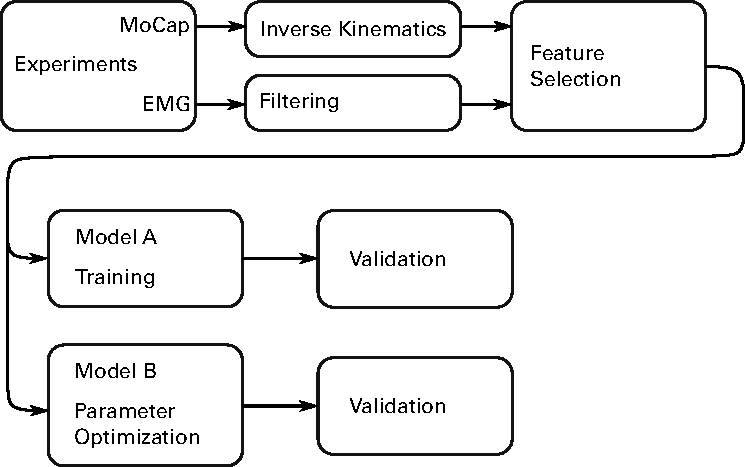
\includegraphics[width=0.8\textwidth]{images/summer_school_study/schematitc.pdf}%
  \caption{Upper Arm Movement Modeling:\\ Schematic workflow of data processing. In experiments, Motion Capture (MoCap) data and EMG signals were recorded. They were processed using inverse kinematics and filtering techniques, respectively. The size of the large datasets was reduced by selecting specific features. Those were used as training inputs for the two models A and B. The trained models were validated using a validation dataset that also originated from experiments.}%
  \label{fig:schematitc}%
\end{figure}%
%
I contributed mainly to the fields of data processing, especially filtering of EMG signals and feature selection, derivation and training of both models, A and B, their validation and the overall programming and visualization of the results. The respective fields are presented more detailed in the following, corresponding sections.

\subsection{Structure of this Chapter}
\Cref{sec:exp_study} gives an overview of the experiments, data processing and feature selection, which resulted in the required datasets. In \cref{sec:study_models}, the two models, A and B, are described. Results including the validation of the models and a discussion are given in \cref{sec:evaluation}. Conclusions follow in \cref{sec:study_conclusion}.

\section{Experimental Study}\label{sec:exp_study}

\begin{figure}%
    \centering%
    \def\svgwidth{5cm}%
    \input{images/summer_school_study/summer_school_study.pdf_tex}%
    \caption{Upper Arm Movement Modeling: \\Experimental setup for the triceps trials. The subject pulls down a rope over a pulley which is connected to a weight with mass $m_w$.
    Angles required for the kinematic formulation are the elbow angle, $\phi_e$, the forearm angle, $\phi_a$, and the angle of the weight, $\phi_w$. The length of the ulna bone is denoted by $\ell_u$.}%
    \label{fig:summer_school_study}%
\end{figure}%

Experiments are required to identify the model parameters for the particular subject. First, the experimental setup is described, then, details on the processing of the measured values are given. Then, the selection of feature points from the experimental data is described.

\subsection{Experimental Trials}

In a series of experiments, eight different actions of flexing and extending the elbow were performed by the subject. Weights of 3 kg and 5 kg were held in the hand during the elbow flexion trials. For the elbow extension trials, a pulley system was installed that redirected the force of the weight such that the downward movement of the forearm acted against the direction of the force. This is shown in \cref{fig:summer_school_study}. A detailed description of the experimental trials can be found in \cite{summerschool2019}.

Time series of position and velocity of the upper arm and the forearm were recorded using a Motion Capture system. It consisted of eight cameras that tracked three markers placed on shoulder, elbow and wrist of the subject. 

The elbow torque $\tau$ was computed as
\begin{equation*}
  \begin{array}{lll}
    \tau = m_w\,g\,\ell_u\,\sin(\phi_w) - m_{a}\,g\,\dfrac{\ell_u}{2}\,\sin(\phi_a),
  \end{array}
\end{equation*}
where $(m_w\,g)$ is the force of the weight, $m_{a}$ is the mass of forearm and hand, $\ell_u$ is the length of the ulna bone and $\phi_a$ and $\phi_w$ are the angles of the forearm and rope, as visualized in \cref{fig:summer_school_study}.

\subsection{Data Processing}
From the captured data, derived quantities of biceps ($B$) and triceps ($T$) muscles were estimated using a geometric model of the upper arm. 
The geometric model is available in the software OpenSim \cite{OpenSim2007} and was customized for the particular subject. The inverse kinematics module of OpenSim was used to estimate the muscle tendon unit lengths, $\ell_{\text{MTU},M}$, contraction velocities, $v_M=\dot{\ell}_M$, and moment arms, $r_{M}$, of the two muscles, $M\in\{B,T\}$.

EMG signals were captured by two electrodes on the skin at the biceps and triceps muscles. For both signals, several preprocessing steps were applied to obtain the inputs for the two models, A and B.

The raw signal was filtered with the same procedure as in \cite{Falisse2016}. First, a fourth-order Butterworth high pass filter with cutoff frequency 30 Hz was applied to reduce non-zero average voltages. Second, the resulting signal was full-wave rectified by taking the absolute value of every measured data point. Third, application of a fourth-order Butterworth low pass filter with 10 Hz cutoff frequency yielded a smoothed signal.
Forth, the resulting filtered EMG signals were normalized to the interval $[0,1]$, such that the value of 1 corresponds to the experimentally determined value of maximum voluntary contraction.

The measured EMG signals on the skin directly correspond to the electric excitation level $u$ in the muscle. Excitation leads to the release of free calcium ions within the sarcomere. Binding of calcium ions to myosin increases the concentration of cross-bridges. This concentration is commonly known as the muscular activation $\alpha$. The muscular activation directly corresponds to the produced force of the muscle \cite{Bayer2017}.

The concentration of free calcium ions is denoted as $\gamma$ and can be computed from the excitation $u$ by the following first order differential equation \cite{Hatze1977}
%
\begin{equation*}
  \begin{array}{lll}
    \dot{\gamma} = m\,(u - \gamma).
  \end{array}
\end{equation*}
%
We used the filtered EMG signal $u$ to obtain values for $\gamma$. \Cref{fig:emg_filtering} shows the raw and filtered EMG signals and the resulting free calcium concentration for a sample of the experimental data.

\begin{figure}%
  \centering%
  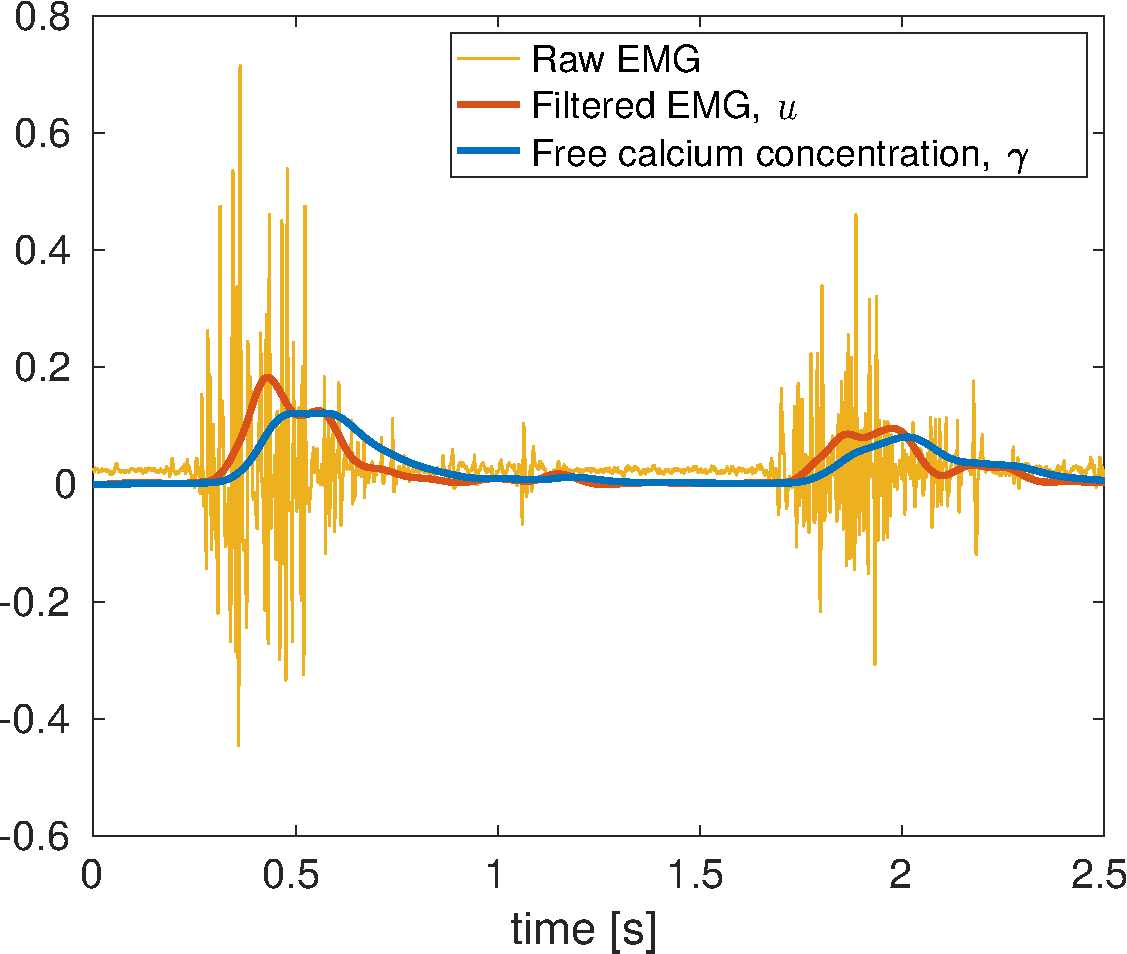
\includegraphics[width=0.8\textwidth]{images/summer_school_study/emg_filtering.pdf}%
  \caption{From raw EMG data of the biceps (yellow) to the filtered signal $u$ (red) and the free calcium concentration $\gamma$ (blue). The data are taken from the beginning of the first elbow flexion experiment. It can be seen that the filtering smooths out the initial signal and removes the constant offset. The free calcium ion concentration follows the filtered EMG with a short delay.}%
  \label{fig:emg_filtering}%
\end{figure}%

The activation of the muscle $\alpha$ does not only depend on the free ion concentration $\gamma$ but also on the current state of muscle contraction. This excitation-contraction coupling has to be described by a dynamic system of ODEs and is included in model B.
Therefore, preprocessing is completed with computing the free calcium concentration $\gamma$ and not the activation $\alpha$.

\subsection{Feature Selection} \label{sec:study_feature_selection}

The eight experimental trials were split into $n_\text{trials}=7$ experiments to be used for model identification and one for validation.
The total number $N$ of captured values in the training experiments was large, such that not all points could be used for training of models A and B.
To reduce the amount of data and, thus, speed up the computation, we selected $n \ll N$ featured values with the assumption that they are representative for the whole data set.
For every experimental trial, we choose the same fixed number $n_\text{per\_trial}$ of data points.
Our selection algorithm identifies $n_\text{per\_trial}$ timesteps, $t_i, i=1, \dots, n$ such that the summed values of the free calcium concentrations $\gamma_B(t_i) + \gamma_T(t_i)$ for biceps and triceps are evenly distributed along the value range.
This leads to $n = n_\text{trials} \cdot n_\text{per\_trial}$ selected data points.

The set of training data $\mathcal{D} = \mathcal{X} \times \mathcal{Y}$ consists of the $n$ selected vectors of the experimental values that are the input to the system of muscles, $\bfx_i \in \mathcal{X}, i=1,\dots, n$, together with the observed output values, $y_i \in \mathcal{Y}, i=1,\dots,n$.
The input vectors contain values for muscle tendon unit lengths, contraction velocities, moment arms and free calcium ion concentrations for biceps and triceps each, $\bfx_i = (\ell_{\text{MTU},B}, \ell_{\text{MTU},T}, v_B, v_T, r_{B}, r_{T}, \gamma_B, \gamma_T)^\top(t_i)$. The output values consist of the elbow torques, $y_i = \tau(t_i)$. This data set, $\mathcal{D}$, serves as training input for both models, A and B.

\section{Models}\label{sec:study_models}

The current section describes the two model approaches that can predict elbow torques from experimental input data. \Cref{sec:data_driven_model} introduces the non-parametric, data driven model A. \Cref{sec:biophysical_model} presents the biophysically based model B. It requires a parameter optimization, which is described in \cref{sec:parameter_optimization}.

\subsection{Data-driven Model A}\label{sec:data_driven_model}

The first modeling approach uses a non-parametric model. Such a model approximates the function $f$ that maps from input to output data points. The function $f$ is learned from the training data set. Regression is used to obtain predictions for new data points. In our case, we use a stochastic model that considers the probability distribution of the model function.

We use the method of \emph{Gaussian Process Regression}. A Gaussian process is a collection of random variables such that the joint distribution of every finite subset of these random variables is multivariate normal (Gaussian).
In our example, each input data point in the space of measured values, $\bfx \in \mathcal{X}$ has an associated random variable $f(\bfx)$ that describes the output of the model for this point.

A Gaussian process, $\mathcal{GP}$, is characterized by a mean function $m(\bfx)$ and a kernel function $k(\bfx,\bfx')$ that models the covariance between any pair $(\bfx, \bfx') \in \mathcal{X} \times \mathcal{X}$ of points. Different choices of kernel functions are possible and can depend on hyperparameters $\bfpsi$. Describing observed values $y$ by a Gaussian process distribution can be expressed as
\begin{equation*}
  \begin{array}{lll}
    f(x) \approx y \sim \mathcal{GP}\big(m(\bfx), k(\bfx,\bfx',\bfpsi)\big).
  \end{array}
\end{equation*}
This representation is non-parametric in the sense that no particular parametric form of the function $y=f(\bfx)$ is assumed whose (biophysical) parameters would be determined. Instead, a generic probabilistic model is constructed using the observed function values at measured inputs $\bfx_i \in \mathcal{X}$.
%More specifically, the conditional distribution $p(y|\bfx)$ considered.

Gaussian Process Regression is based on \emph{Bayesian Inference} to update a prior belief of the model to a posterior model using information contained in observations of the process.
The observed data are the set of measurements $\mathcal{D}$. 

The \emph{prior} distribution $p(\bff\mid\mathcal{X},\bfpsi)$ for the vector of function values $\bff$ is described by the Gaussian process,
\begin{equation*}
  \begin{array}{lll}
    p(\bff\mid\mathcal{X},\bfpsi) = \mathcal{N}(\bff\mid\bfm,\bfK),
  \end{array}
\end{equation*}
with mean values $\bfm = (m(\bfx_i))^\top_{i=1,\dots,n}$ and covariance matrix $\bfK$ with $K_{ij} = k(\bfx_i,\bfx_j,\bfpsi).$

The \emph{likelihood} $p(\bfy\mid f(\bfx), \bftheta)$ describes the probability of an observation $\bfy$ given a particular model $f$. The vector $\bftheta$ denotes additional parameters of the likelihood. 

Using Bayes' rule, the \emph{posterior} distribution $p(\bff\mid\mathcal{D})$ of the function values $\bff$ can be computed from prior and likelihood as
\begin{equation*}
  \begin{array}{lll}
    p(\bff\mid\mathcal{D},\bftheta,\bfpsi) 
      = \dfrac{p(\bfy\mid\bff,\bftheta)\,p(\bff\mid\mathcal{X},\bfpsi)}{p(\mathcal{D}\mid\bftheta,\bfpsi)}.
  \end{array}
\end{equation*}
This results in a measure for the uncertainty of the model $f$ at unobserved points $\bfx_\ast \notin \mathcal{D}$. 

Additionally, the fact that the measured quantities in the experiments are subject to measurement noise can be incorporated into the model.
The assumption 
\begin{equation*}
  \begin{array}{lll}
    y = f(\bfx) + \eps
  \end{array}
\end{equation*}
adds a normally distributed random variable of observational noise $\eps \sim \mathcal{N}(0,\sigma_n^2)$ to the formulation. The noise variance $\theta = \sigma_n^2$ is an additional parameter of the likelihood. 
It is also possible to explicitly model the mean function $m(\bfx)$. By replacing the model $f(\bfx)$ by $g(\bfx) = f(\bfx) + \bfh(\bfx)^\top \bfbeta$, i.e.
\begin{align*}
  %\begin{array}{rlrl}
    y &= f(\bfx) + \bfh(\bfx)^\top \bfbeta + \eps, \quad 
    &\text{ with } f(x) &\sim\mathcal{GP} \big(m(\bfx), k(\bfx,\bfx',\bfpsi)\big),\\[4mm]
    && \eps &\sim \mathcal{N}(0,\sigma_n^2),
  %\end{array}
\end{align*}
we allow for a global trend in the data that is formulated in terms of a vector of explicit basis functions $\bfh(\bfx)$ and corresponding coefficients $\bfbeta$.

The algorithm for Gaussian Process Regression involves estimating the following values from the given data during the training phase. The hyperparameters of the covariance function $\bfpsi$, the noise variance $\bftheta$, and the coefficients of the fixed basis functions $\bfbeta$ are determined by solving an optimization problem. The computation involves matrix inversions and has a computational complexity $\O(n^3)$, i.e. is cubic in the number of data points. For details, the reader is referred to the literature \cite{Rasmussen2005,kuss2006gaussian}.

In our study, training of the Gaussian Process of model A was performed using the ready to use implementation provided by MATLAB.
We parametrized the covariance by a squared exponential kernel and used constant basis functions, $\bfh(x) = 1$. We enabled observational noise, its variance $\bftheta = \sigma_n^2$ was found by optimization during training of the model.

%$p(\bff^\ast | \mathcal{D},\mathcal{X}^\ast)$
\subsection{Biophysical Model B}\label{sec:biophysical_model}

Extension of the elbow is governed by the triceps brachii muscle.
During elbow flexion, three muscles are involved: biceps brachii, brachialis and brachioradialis. For simplicity, only biceps brachii, which contributes most of the moment, is explicitly considered in the current study. The effects of the other two muscle are contained in the biceps brachii model in a lumped manner.

Thus, the biophysical model consists of two Hill-type muscle models, for biceps and triceps, respectively. The muscle models are arranged around a hinge joint for the elbow angle. The muscle forces contribute to the torque at the elbow over their respective moment arms.

Hill-type models describe the macroscopic, dynamic mechanical behavior of an entire muscle along a one-dimensional line of action.
The behavior is formulated by phenomenological, mathematical functions that have to be parametrized to fit experimental observations.

%Such models are often used to compute muscle forces in simulations of various movements, e.g. \cite{Siebert2003}, \cite{Kistemaker2006}.
Multiple variants of Hill-type models exist that use various configurations of mechanical elements to consider different properties and functionalities of the muscle. The original model was proposed in \cite{Hill1938}. It contains a contractile element (CE) and two elastic elements, arranged in series and in parallel to the CE.
The authors of \cite{Siebert2008} compare two different approaches using these three elements. The effect of tension in eccentric contractions is added to the Hill-type model by \cite{Till2008}. The authors of \cite{Gunther2007} add a forth, damping element to account for high-frequency damping of the muscle tissue. In \cite{Morl2012}, electromechanical delay is investigated with and without the additional damping element. 

\begin{figure}%
  \centering%
  \def\svgwidth{0.5\textwidth}
  \input{images/summer_school_study/hilltype.pdf_tex}%
  \caption{Mechanical structure of the Hill-type muscle model. The force generating contractile element (CE) is parallel-connected to the parallel elastic element (PEE) and connected in series to a second parallel-connected structure consisting of the serial elastic element (SEE) and the serial damping element (SDE). The length $l_\text{MTU}$ of the whole muscle tendon unit is composed of the common length $l_\text{CE}$ of CE and PEE and the common length $l_\text{SEE}$ of SEE and SDE. The variable $l_\text{CE}$ is an internal state of the model.}
  \label{fig:hilltype}%
\end{figure}%

\newcommand{\CE}{\text{CE}}
\newcommand{\MTU}{\text{MTU}}

We employ the four-element Hill-type muscle model that is described by \cite{Hilltype2014}. Its structure is visualized in \cref{fig:hilltype}. It consists of four components: the contractile element (CE), the parallel elastic element (PEE), the serial elastic element (SEE), and the serial damping element (SDE). Inputs to the model are the muscular activation $\alpha(t)$, the length $l_\MTU(t)$ and the contraction velocity $\dot{l}_\MTU(t)$ of the muscle tendon unit (MTU).
The output of the model is the muscle force $f_\text{MTU}(t)$. The model contains one internal state variable, the length $l_\text{CE}(t)$ of the CE. The muscle dynamics determine this internal length and its time derivative, the contraction velocity $\dot{l}_\text{CE}(t)$ of the CE.

The resulting force of the MTU is given as sum of the forces of the respective parallel elements as visualized in \cref{fig:hilltype}:
\begin{equation}\label{eq:hill_type0}
  \begin{array}{lll}
    F_\MTU = F_\CE(l_\CE, \dot{l}_\CE, \alpha) + F_\text{PEE}(l_\CE) = F_\text{SEE}(l_\CE,l_\MTU) + F_\text{SDE}(l_\CE,\dot{l}_\CE,\dot{l}_\MTU,\alpha).
  \end{array}
\end{equation}
The force terms of the four elements, $F_\CE, F_\text{PEE}, F_\text{SEE}$ and $F_\text{SDE}$ are described by analytical functions that use a total of 19 parameters. A description of the detailed equations and parameters can be found in \cite{Hilltype2014}. In the following, an overview over the formulation is given with a focus on the piecewise formulated terms that contribute to the overall muscle model. In the following formulations, underlined variables designate constant parameters that either have to be specified or follow from other given parameters.

The muscle output force $F_\text{MTU}$ is computed by the second identity of \cref{eq:hill_type0}, i.e., from the forces $F_\text{SEE}$ and $F_\text{SDE}$. The force $F_\text{SEE}$ acting in the SEE is formulated as a continuous piecewise function with a constant zero, an exponential and a linear branch:
\begin{equation*}
  \begin{array}{lll}
    F_\text{SEE}(\ell_\CE,\ell_\MTU) = \begin{cases}
      0, & \ell_\text{SEE} < \underline{l_{\text{SEE},0}}\\[2mm]
      \underline{K_\text{SEE,nl}}(\ell_\text{SEE} - \underline{\ell_\text{SEE,0}})^{\underline{\nu_\text{SEE}}}, & \ell_\text{SEE} < \underline{\ell_\text{SEE,nll}}\\[2mm]
    \underline{\Delta F_\text{SEE,0}} + \underline{K_\text{SEE,l}}(\ell_\text{SEE} - \underline{\ell_\text{SEE,nll}}), & 
    \ell_\text{SEE} \geq \underline{\ell_\text{SEE,nll}}
    \end{cases}, \quad \text{with } \ell_\text{SEE} = \ell_\MTU - \ell_\CE.
  \end{array}
\end{equation*}

The damping force $F_\text{SDE}$ in the SDE is proportional to the lengthening velocity ${\dot{\ell}_\text{SEE} = \dot{\ell}_\MTU - \dot{\ell}_\CE}$ of this element. It is given by
\begin{equation}\label{eq:sde_force}
  \begin{array}{lll}
    F_\text{SDE}(l_\CE,\dot{l}_\CE,\dot{l}_\MTU,\alpha) \\ \qquad = \underline{D_\text{SDE,max}}\left( (1-\underline{R_\text{SDE}}) \dfrac{F_\text{PEE}(\ell_\CE)+F_\text{CE}(\ell_\CE, \dot{\ell}_\CE, \alpha)}{\underline{F_\text{max}} + \underline{R_\text{SDE}}} \right) (\dot{\ell}_\MTU - \dot{\ell}_\CE).
  \end{array}
\end{equation}
The amount of damping is dependent on the force $F_\MTU$ of the MTU which appears in the nominator of the fraction in \cref{eq:sde_force} as the sum of the forces $F_\text{PEE}$ and $F_\CE$. Formulas for these two forces are given in the following.

The force $F_\text{PEE}$ of the PEE is formulated piecewise as a shifted and cut off polynomial function:
\begin{equation}\label{eq:fpee}
  \begin{array}{lll}
    F_\text{PEE}(\ell_\CE) = \begin{cases}
      0, & \ell_\CE < \underline{\ell_{\text{PEE},0}}\\[4mm]
    \underline{K_\text{PEE}}(l_\CE - \underline{l_{\text{PEE},0}})^{\underline{\nu_\text{PEE}}},& \ell_\CE \geq \underline{\ell_{\text{PEE},0}}
    \end{cases}.
  \end{array}
\end{equation}

The force $F_\CE$ of the CE is the active force produced by the muscle and is given by:
\begin{equation}\label{eq:fce}
  \begin{array}{lll}
    F_\CE(l_\CE, \dot{l}_\CE, \alpha) 
    = \underline{F_\text{max}} \left(
    \dfrac{\alpha\,F_\text{isom}(\ell_\CE) + A_\text{rel}(\dot{\ell}_\CE,\ell_\CE,\alpha)}
    {1 - 
    \frac{\dot{\ell}_\CE}
    {B_\text{rel}(\dot{\ell}_\CE,\ell_\CE,\alpha)\,\ell_{\CE,\text{opt}}}}\right)
    - A_\text{rel}(\dot{\ell}_\CE,\ell_\CE,\alpha).
  \end{array}
\end{equation}
It can be seen that the active force depends on the activation level $\alpha$. 
The formulation of $F_\CE$ contains the two main characteristic curves for muscle forces, the force-length relation and the force-velocity relation.

The force-length relation is modeled by the function $F_\text{isom}(\ell_\CE)$ of isometric force, which describes the relative force for the condition $\dot{\ell}_\CE = 0$. This function is formulated piecewise for CE lengths $\ell_\CE$ smaller and larger than an optimal length $\ell_\text{CE,opt}$. 

The force-velocity relation follows from the auxiliary functions $A_\text{rel}(\dot{\ell}_\CE,\ell_\CE,\alpha)$ and $B_\text{rel}(\dot{\ell}_\CE,\ell_\CE,\alpha)$. These functions have different forms for concentric ($\dot{\ell}_\CE < 0$) and eccentric ($\dot{\ell}_\CE \geq 0$) conditions as well as for the two ranges of CE  length, $\ell_\CE < \ell_\text{CE,opt}$ and $\ell_\CE \geq \ell_\text{CE,opt}$.

\begin{figure}%
  \centering%
  \begin{subfigure}[t]{0.9\textwidth}%
    \centering%
    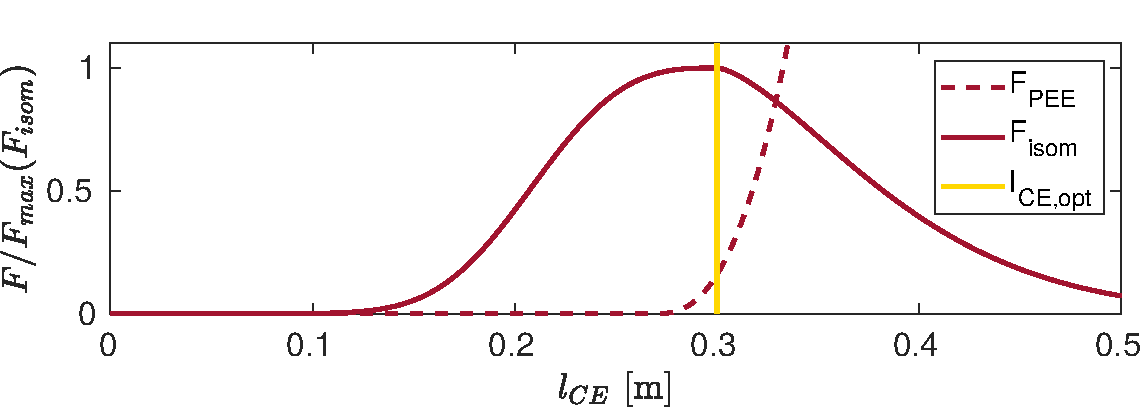
\includegraphics[width=\textwidth]{images/summer_school_study/force_curves_generic_length.pdf}%
    \caption{Force-length curves of the PEE (dashed red line) and isometric force $F_\text{isom}$ (solid red line) for an isometric condition ($\dot{l}_\CE=0$), normalized to the maximum isometric force. The optimal length $l_\text{CE,opt}$ of the CE is shown as yellow vertical line. The force $F_\text{PEE}(l_\CE)$ of the PEE is zero for $l_\CE < 0.9\,l_\text{CE,opt}$. The isometric contraction force $F_\text{isom}$ is formulated piecewise by two branches separated by $l_\text{CE,opt}$.}%
    \label{fig:force_curves_generic_length}%
  \end{subfigure}\\[6mm]
  \begin{subfigure}[t]{0.9\textwidth}%
    \centering%
    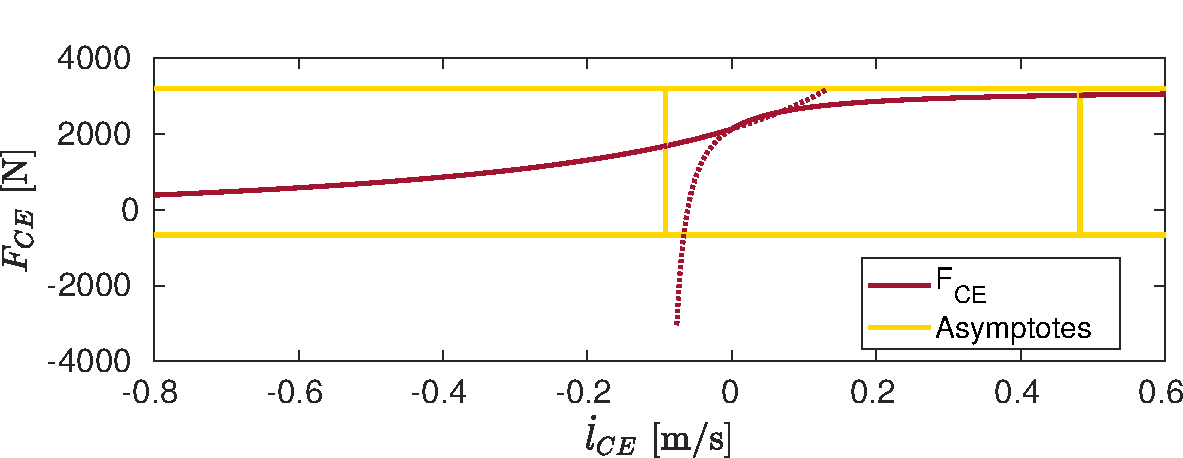
\includegraphics[width=\textwidth]{images/summer_school_study/force_curves_generic_velocity.pdf}%
    \caption{Force-velocity curve $F_\CE(\dot{l}_\CE)$ of the CE at optimal length $l_\CE=l_{\CE,\text{opt}}$, and for activation level $\alpha=0.5$. The function (red solid line) is formulated piecewise, graphs of the base functions of the two branches continue as red dotted lines. Their limits and singularities are visualized by the yellow horizontal and vertical asymptotes.}%
    \label{fig:force_curves_generic_velocity}%
  \end{subfigure}%
  \caption{Force-length and force-velocity relations for the muscle model with generic parameters taken from literature \cite{Hilltype2014}.}%
  \label{fig:force_curves_generic}%
\end{figure}%

\Cref{fig:force_curves_generic} visualizes the two main characteristic curves of the model. 
\Cref{fig:force_curves_generic_length} shows how the generated force depends on the length of the CE. 
The active force $F_\CE$, given by \cref{eq:fce}, is visualized by the solid red line. It has its maximum at the optimal length $l_\text{CE,opt}$ of the CE. This can be explained by the overlap of actin and myosin filaments in the sarcomere. The overlap is lower when the actin filaments are pulled apart or pushed together. A higher overlap leads to a higher force output.

The dashed line in \cref{fig:force_curves_generic_length} represents the passive force $F_\text{PEE}$ of the elastic muscular tissue, formulated in \cref{eq:fpee}. The passive force is essentially generated by the titin proteins in the sarcomere. Only starting from a certain length, the structure exerts reaction forces against lengthening forces to avoid overstretching of the muscle.

\cref{fig:force_curves_generic_velocity} shows the force-velocity relation of the Hill-type model. The curve of $F_\CE(\dot{l}_\CE)$ is composed of two branches: 
The concentric branch for shortening contraction with $\dot{l}_\CE \leq 0$ and the eccentric branch for lengthening contraction with $\dot{l}_\CE > 0$. It can be seen that the generated force increases monotonically over the lengthening velocity. It approaches a limit for maximum positive and negative velocity. These limits can be adjusted by parameters of the model and are exemplary for how the shape of the curves of a Hill-type model can be parametrized.

In addition to the resulting muscle force $F_\MTU$, a formulation for the internal state variable $\ell_\CE$ is required.
The second identity of \eqref{eq:hill_type0} can be solved for the lengthening velocity $\dot{\ell}_\CE$ of the CE to get an evolution equation for the length $\ell_\CE$ of the CE. The derivation and the resulting formula can be found in \cite{Hilltype2014}.

To describe the activation dynamics, i.e., the evolution of the muscle activation ${\alpha \in [0,1]}$, the model of Hatze et al. \cite{Hatze1977} is used.
The activation is computed depending on the free calcium ion concentration $\gamma$ and the length $\ell_\CE$ of the CE by
\begin{equation*}
  \begin{array}{lll}
    \alpha(\ell_\CE,\gamma) = \dfrac{\underline{a_0} + \big(\rho(\ell_\CE)\,\gamma\big)^3}
    {1 + \big(\rho(\ell_\CE)\,\gamma\big)^3}.
  \end{array}
\end{equation*}
The function $\rho$ is given by
\begin{equation*}
  \begin{array}{lll}
    \rho(\ell_\CE) = \underline{c}\,\underline{\eta}\,\dfrac{(\underline{k}-1)\,\ell_\CE}{(\underline{k} - \ell_\CE/\ell_\text{CE,opt})\,l_\text{CE,opt}}.
  \end{array}
\end{equation*}
All used parameter values for the activation dynamics can be found in \cite{Bayer2017}.

In summary, we get the following coupled system of differential-algebraic equations, where $f_\CE$ and $f_\alpha$ denote the respective formulas:
\begin{align}
  F_\MTU &= F_\MTU(\ell_\MTU,l_\CE,\dot{l}_\CE,\alpha),      \label{eq:hill_type1} \\[4mm]
  \dot{l}_\CE &= f_\CE(l_\CE,\ell_\MTU,\dot{l}_\MTU,\alpha), \label{eq:hill_type2}\\[4mm]
  \alpha &= f_\alpha(\gamma, l_\CE).                      \label{eq:hill_type3}
\end{align}

To compute the joint torque in a system of an agonist and antagonist muscle pair, two instances of the presented Hill-type muscle model can be used. In our study considering the upper arm, the torque $\tau$ at the elbow is computed by multiplying the predicted forces $F_{\MTU,B}$ and $F_{\MTU,T}$ of biceps and triceps with the corresponding moment arms $\hat{r}_B$ and $\hat{r}_T$:
\begin{equation}\label{eq:muscle_torque}
  \begin{array}{lll}
    \tau = F_{\MTU,B}(l_{\MTU,B},\dot{l}_{\MTU,B},\alpha_B) \cdot \hat{r}_B - F_{\MTU,T}(l_{\MTU,T},\dot{l}_{\MTU,T},\alpha_T) \cdot \hat{r}_T.
  \end{array}
\end{equation}

\subsection{Parameter Identification for Model B}\label{sec:parameter_optimization}
%
The process of model identification finds the parameters that make the model B predict correct values for the specific subject, i.e., minimizes the error in the predicted outcome for the training data set.

The following minimization is performed:
\begin{align}
  &&\min\limits_{\substack{\bftheta_M,l_{\CE,M}(t), \\\forall M \in \{B,T\}, \,\forall t \in \mathcal{T}}} &\sum\limits_{t\in \mathcal{T}}|\tau(t) - \hat{\tau}(t)|^2
   \label{eq:opt_1}\\[4mm]
  &&\text{s.t. }\forall t \in \mathcal{T}:\quad &\tau(t) = F_{\MTU,B}(t,l_{\CE,B},\bftheta_B) \cdot \hat{r}_B(t) \notag\\
      &&&\qquad\quad- F_{\MTU,T}(t,l_{\CE,T},\bftheta_T) \cdot \hat{r}_T(t),                 \label{eq:opt_2}\\[4mm]
  &&& \dot{l}_{\CE,M}(t) = \dot{\hat{l}}_{\MTU,M}(t),\quad M \in \{B,T\},      \label{eq:opt_3}\\[4mm]
  &&& \bftheta_B, \bftheta_T \in \Theta,                                       \label{eq:opt_4}\\[4mm]
  &&& l_{\CE,M}(t) \in [0,l_{\MTU,M}(t)],\quad M \in \{B,T\}.                  \label{eq:opt_5}
\end{align}

The optimization variables are the parameters $\bftheta_B$ and $\bftheta_T$ for the biceps and triceps Hill-type models and the lengths $l_{\CE,B}(t)$ and $l_{\CE,T}(t)$ of the contractile elements for both models at every point in time. The variables designated as $\hat{\square}$ are the measured quantities from the training experiments. The objective function given in \cref{eq:opt_1} penalizes the difference between computed torque $\tau$ and measured torque $\hat{\tau}$ at every timestep $t \in \mathcal{T}$ of the training data. 

\Cref{eq:opt_2} computes the torque values and follows from \cref{eq:muscle_torque} of the muscle model. For every point in time, the predicted forces $F_{\MTU,B}$ and $F_{\MTU,T}$ are multiplied with the measured moment arms $\hat{r}_B$ and $\hat{r}_T$.

In \cref{eq:opt_3}, the contraction velocities are constrained to the measured values. Because the lengthening velocity $\dot{l}_\CE$ of the CE is an internal quantity and, thus, cannot be observed in experiments, we assume it to be equal to the lengthening velocity of the whole muscle: $\dot{l}_\CE \approx \dot{l}_{\MTU} = \dot{l}_\text{CE} + \dot{l}_\text{SEE}$. This requires the assumption $\dot{l}_{\text{SEE}} \approx 0$ which can be justified given the low dynamic nature of the experiments.

By \cref{eq:opt_4}, we bound each of the parameters $\bftheta_B$ and $\bftheta_T$ to a range between half and twice the generic value from literature.
The lengths of the CEs are constrained by \cref{eq:opt_5} to be positive and smaller than the length of the MTU.

All optimization variables are normalized to improve the numerical conditioning of the optimization problem. 
The parameters $\bftheta_B$ and $\bftheta_T$ are normalized with respect to generic values from literature that were taken from \cite{Gunther2007, Morl2012, Hilltype2014}. The initial values are set to one, which corresponds to the generic literature values.
The internal states $l_{\CE,B}$ and $l_{\CE,T}$, are normalized with respect to the measured MTU lengths $\hat{l}_{\MTU,B}$ and $\hat{l}_{\MTU,T}$ and initialized with zero.

%For training of model B, the optimization problem for the parameters needed to be solved. 
We implemented the Hill-type models and the constraints in MATLAB and used the nonlinear programming implementation, \code{fmincon}, to minimize the given bounded and nonlinear constrained, multivariable function.
In our study, the total number of optimization variables is computed by $2\cdot 19 + 2n = 598$, as each of the parameter vectors $\bftheta_B,\bftheta_T$ had 19 entries. 

\section{Results and Discussion}\label{sec:evaluation}

In the following, results of connecting the two model formulations, A and B, to the experimental data are presented.
At first, \cref{sec:res_feature_selection} gives details on the preprocessed data. The training phase is described in \cref{sec:res_training}. Applying the trained models to the validation data is done in \cref{sec:res_validation}. Then, \cref{sec:res_simplified_a} tests a simplified version for model A. Then, \cref{ref:res_insights_b} shows some insights into the optimized parameter values for model B.

\subsection{Feature Selection}\label{sec:res_feature_selection}
% intro
The experimental data is split into a training and a validation dataset. \Cref{fig:selected_points} shows the processed data of the training data set. In total, we captured $N=\num{34934}$ data points for the seven experimental trials. Out of these, we select $n_\text{per\_trial}=\num{40}$ feature points in every trial, leading to a total of $n=n_\text{per\_trial}\cdot n_\text{trials}=\num{280}$ points. The selected points are visualized by crosses in the top plot of \cref{fig:selected_points}. It can be seen that the algorithm described in \cref{sec:study_feature_selection} distributes the feature points equally along the $\gamma$ axis.

\begin{figure}%
  \centering%
  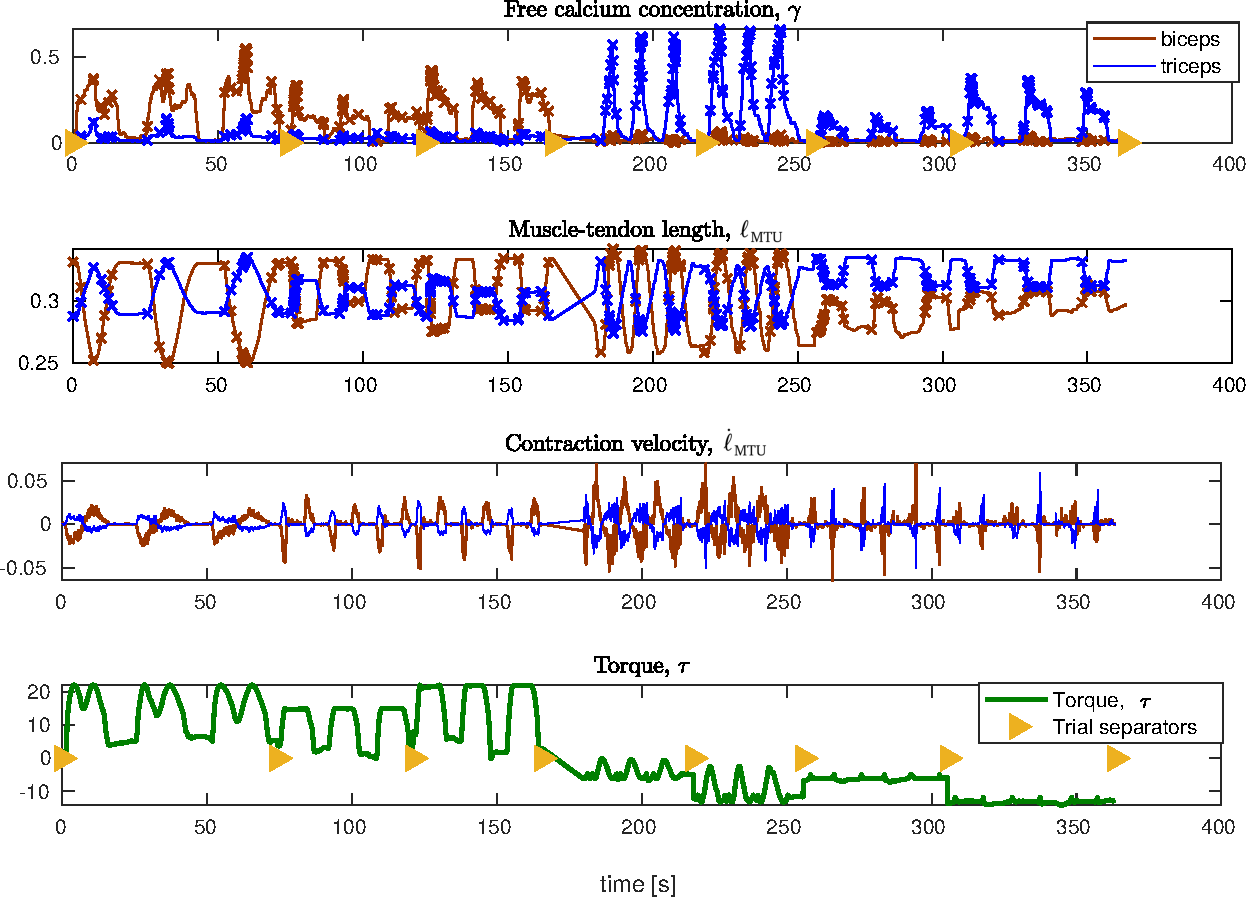
\includegraphics[width=\textwidth]{images/summer_school_study/selected_points.pdf}%
  \caption{Processed experimental values over time that were used for training of both models. The concatenated data of seven trials are shown, which yield an end time of $\SI{363.32}{s}$. The individual trials are separated by the yellow triangles on the $x$-axis. The three upper plots show the values of $\gamma, \ell_\MTU$ and $\dot{l}_\MTU$ for both biceps (brown) and triceps (blue), the bottom plot shows the elbow torque $\tau$. The selected feature points are visualized as crosses in the two top plots. In the upper-most plot, it can be seen that the first three trials, which correspond to elbow flexion, mainly activated the biceps muscle, whereas in the last four trials, corresponding to elbow extension, the triceps is more active.
}%
  \label{fig:selected_points}%
\end{figure}%

\subsection{Training of the Models}\label{sec:res_training}
%
Training of model A consists of estimating the hyperparameters for the Gaussian Process Regression model from the training data.

For model B, the optimization problem for the biophysical parameters is solved. The resulting parameter values and their relation to the initial values are summarized in \cref{tab:model_b_parameters}. It can be seen that none of the final parameter values is limited by the constraints, which would be $\SI{-50}{\percent}$ and +\SI{100}\percent. However, it was observed that including the constraints helps the optimizer to stay in the valid range of meaningful model parameters and, thus, reach the optimum faster.

\begin{table}[t] 
  \centering
  %\begin{scriptsize}
  
    \begin{tabular}{@{}llllll@{}}
%\hline
 %| param              | biceps   |            | triceps  |            %|
 %| ------------------ | -------- | ---------- | -------- | ---------- %|
 %| CE_F_max           | +11.03 % | 4729.97    | -49.04 % | 2171.04    |
 %| CE_l_CEopt         | +31.72 % | 0.40       | -25.36 % | 0.22       |
 %| CE_DeltaW_limb_des | +10.86 % | 0.39       | +10.86 % | 0.39       |
 %| CE_DeltaW_limb_asc | +91.61 % | 0.67       | +5.05 %  | 0.37       |
 %| CE_v_CElimb_des    | +10.86 % | 1.66       | +10.86 % | 1.66       %|
 %| CE_v_CElimb_asc    | -46.39 % | 1.61       | +95.87 % | 5.88       |
 %| CE_A_rel0          | +14.03 % | 0.29       | -20.34 % | 0.20       |
 %| CE_B_rel0          | +77.51 % | 3.99       | +41.38 % | 3.18       |
 %| CE_S_eccentric     | -4.12 %  | 1.92       | +22.92 % | 2.46       |
 %| CE_F_eccentric     | -30.94 % | 1.04       | +36.79 % | 2.05       |
 %| PEE_L_PEE0         | +10.86 % | 1.00       | +10.86 % | 1.00       |
 %| PEE_l_PEE0         | +10.86 % | 0.30       | +10.86 % | 0.30       |
 %| PEE_v_PEE          | +10.86 % | 2.77       | +10.86 % | 2.77       |
 %| PEE_F_PEE          | +10.86 % | 2.22       | +10.86 % | 2.22       |
 %| PEE_K_PEE          | +10.86 % | 1410470.38 | +10.86 % | 1410470.38 |
 %| SDE_D_SE           | +10.86 % | 0.33       | +10.86 % | 0.33       |
 %| SDE_R_SE           | +8.63 %  | 0.01       | -10.99 % | 0.01       |
 %| SDE_d_SEmax        | +8.41 %  | 513.16     | -10.64 % | 422.98     |
 %| SEE_l_SEE0         | -24.95 % | 0.13       | -10.28 % | 0.15       |
 %| SEE_DeltaU_SEEnll  | +59.16 % | 0.07       | +23.58 % | 0.05       |
 %| SEE_DeltaU_SEEl    | +63.34 % | 0.03       | +19.02 % | 0.02       |
 %| SEE_DeltaF_SEE0    | -42.40 % | 327.16     | +64.75 % | 935.78     |
 
% contractile element (CE)
%===========================
%  CE_F_max                         % F_max in [N] for Extensor (Kistemaker et al., 2006)
%  CE_l_CEopt                       % optimal length of CE in [m] for Extensor (Kistemaker et al., 2006)
%* CE_DeltaW_limb_des = 0.35;       % width of normalized bell curve in descending branch (Moerl et al., 2012)
%* CE_DeltaW_limb_asc = 0.35;       % width of normalized bell curve in ascending branch (Moerl et al., 2012)
%* CE_v_CElimb_des = 1.5;           % exponent for descending branch (Moerl et al., 2012)
%  CE_v_CElimb_asc = 3.0;           % exponent for ascending branch (Moerl et al., 2012)
%* CE_A_rel0 = 0.25;                % parameter for contraction dynamics: maximum value of A_rel (Guenther, 1997, S. 82)
%* CE_B_rel0 = 2.25;                % parameter for contraction dynmacis: maximum value of B_rel (Guenther, 1997, S. 82)
%  eccentric force-velocity relation:
%* CE_S_eccentric  = 2;             % relation between F(v) slopes at v_CE=0 (van Soest & Bobbert, 1993)
%  CE_F_eccentric  = 1.5;           % factor by which the force can exceed F_isom for large eccentric velocities (van Soest & Bobbert, 1993)

% paralel elastic element (PEE)
%===============================
%  PEE_L_PEE0   = 0.9;                               % rest length of PEE normalized to optimal lenght of CE (Guenther et al., 2007)
%  PEE_v_PEE    = 2.5;                               % exponent of F_PEE (Moerl et al., 2012)
%  PEE_F_PEE    = 2.0;                               % force of PEE if l_CE is stretched to deltaWlimb_des (Moerl et al., 2012)

% serial damping element (SDE)
%=============================
%* SDE_D_SE    = 0.3;               % xxx dimensionless factor to scale d_SEmax (Moerl et al., 2012)
%* SDE_R_SE    = 0.01;              % minimum value of d_SE normalised to d_SEmax (Moerl et al., 2012)
%  SDE_d_SEmax = SDE_D_SE*(CE_F_max*CE_A_rel0)/(CE_l_CEopt*CE_B_rel0);
                                    % maximum value in d_SE in [Ns/m] (Moerl et al., 2012)

% serial elastic element (SEE)
% ============================
%  SEE_l_SEE0        = 0.172;       % rest length of SEE in [m] (Kistemaker et al., 2006)
%  SEE_DeltaF_SEE0   = 568;         % both force at the transition and force increase in the linear part in [N] (~ 40% of the maximal isometric muscle force)
%  SEE_DeltaU_SEEnll = 0.0425;      % relativ stretch at non-linear linear transition (Moerl et al., 2012)
%* SEE_DeltaU_SEEl   = 0.017;       % relativ additional stretch in the linear part providing a force increase of deltaF_SEE0 (Moerl, 2012)
% 
     \toprule
    \textbf{CE} 
      & $F_{\mathrm{max}}\,[\mathrm{N}]$
      & $l_{\mathrm{CE},opt}\,[\mathrm{m}]$ 
      & $\Delta W_{d} \,[\;]$ 
      & $\Delta W_{a} \,[\;]$ 
      & $\nu_{\mathrm{CE},d} \,[\;]$ \\  \midrule
    Generic & $4260$ & $0.3$ & $0.35$ & $0.35$ & $1.5$  \\ %\hline
    Biceps  & $+\SI{11.0}{\percent}$ & $+\SI{31.7}{\percent}$ & $+\SI{10.9}{\percent}$ & $+\SI{91.6}{\percent}$ & $+\SI{10.9}{\percent}$  \\ %\hline
    Triceps & $-\SI{49.0}{\percent}$ & $-\SI{25.4}{\percent}$ & $+\SI{10.9}{\percent}$ & $+\SI{5.1}{\percent}$ & $+\SI{10.9}{\percent}$  \\ %\hline 
    \addlinespace[2ex]
    \textbf{CE} 
      &  $\nu_{\mathrm{CE},a} \,[\;]$ 
      & $A_\text{rel,0} \,[\;]$  
      & $B_\text{rel,0} \,[\;]$ 
      & $S_\text{ecc} \,[\;]$ 
      & $F_\text{ecc} \,[\;]$\\  \hline
    Generic & $3.0$ & $0.25$ & $2.25$ & $2$ & $1.5$ \\ %\hline
    Biceps & $-\SI{46.4}{\percent}$ & $+\SI{14.0}{\percent}$ & $+\SI{77.5}{\percent}$ & $-\SI{4.1}{\percent}$ & $-\SI{30.1}{\percent}$ \\ %\hline
    Triceps &  $+\SI{95.9}{\percent}$ & $-\SI{20.3}{\percent}$ & $+\SI{41.4}{\percent}$ & $+\SI{22.3}{\percent}$ & $+\SI{36.8}{\percent}$ \\ %\hline
    \addlinespace[2ex]
    \textbf{PEE} 
      & $L_{\mathrm{PEE},0} \,[\;]$ 
      & $\nu_{\mathrm{PEE}} \,[\;]$ 
      & $F_{\mathrm{PEE}} \,[\;]$
      \\ \hline
    Generic & $0.9$ & $2.5$ & $2.0$  \\ %\hline
    Biceps & $+\SI{10.9}{\percent}$ & $+\SI{10.9}{\percent}$ & $+\SI{10.9}{\percent}$  \\ %\hline
    Triceps & $+\SI{10.9}{\percent}$ & $+\SI{10.9}{\percent}$ & $+\SI{10.9}{\percent}$  \\ %\hline
    \addlinespace[2ex]
    \textbf{SDE} 
      & $D_{\mathrm{SDE}} \,[\;]$ 
      & $R_{\mathrm{SDE}} \,[\;]$ 
      \\ \midrule
    Generic & $0.3$ & $0.01$    \\ %\hline
    Biceps & $+\SI{10.9}{\percent}$ & $+\SI{8.6}{\percent}$   \\ %\hline
    Triceps & $+\SI{10.9}{\percent}$ & $-\SI{11.0}{\percent}$  \\ %\hline
    \addlinespace[2ex]
    \textbf{SEE} 
      & $l_{\mathrm{SEE},0}\,[\mathrm{m}]$ 
      & $\Delta F_{\mathrm{SEE},0} \,[\;]$  
      & $\Delta U_\text{l} \,[\;]$  
      & $\Delta U_\text{nll}\,[\;]$
      \\ \hline
    Generic & $0.172$ & $0.0425$ & $0.017$ & $568$ \\ %\hline
    Biceps & $-\SI{25.0}{\percent}$ & $-\SI{42.4}{\percent}$ & $+\SI{63.3}{\percent}$ & $+\SI{59.2}{\percent}$ \\ %\hline
    Triceps & $-\SI{10.3}{\percent}$ & $+\SI{64.75}{\percent}$ & $+\SI{19.0}{\percent}$ & $+\SI{23.6}{\percent}$ \\ %\hline
    \bottomrule
  \end{tabular}

  \caption{Hill-type muscle model parameters of the four elements: CE, PEE, SDE and SEE, initial values given in literature and relative changes of the optimized values. Further explanations of the parameters and references to literature containing their initial values are given in \cite{Hilltype2014}.}
  \label{tab:model_b_parameters}
  %\end{scriptsize}
\end{table}

After training of the models A and B using the selected points of the training dataset, both models were tested by a \emph{resubstitution prediction}, i.e., predicting output from the training input data. The results are shown in \cref{fig:measured_optimized_torque_A} for model A and \cref{fig:measured_optimized_torque_B} for model B. As this evaluation only uses the subset of selected experimental values, the data points have no natural ordering. They were sorted for better visibility.

It can be seen that, for both models, the predicted values are a good fit to the measured values. For model A, the predicted 95\% confidence interval includes the actually measured values almost everywhere. For model B, the predicted values show a higher variance, especially for high torque values.

\begin{figure}%
  \centering%
  \begin{subfigure}[t]{0.48\textwidth}%
    \centering%
    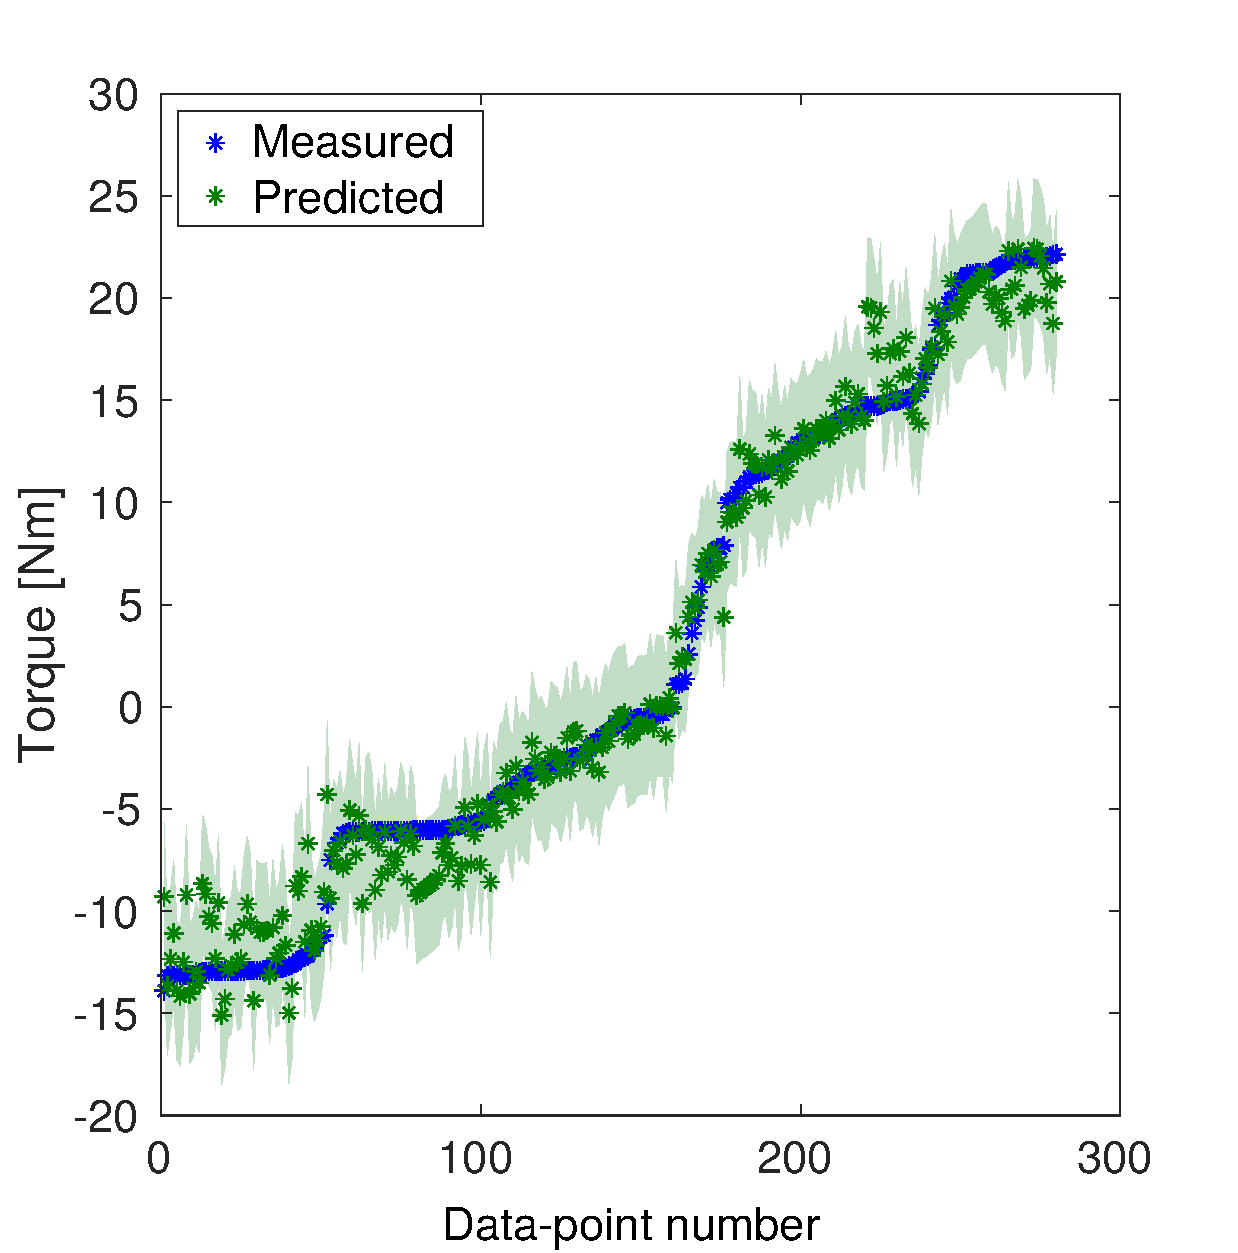
\includegraphics[width=\textwidth]{images/summer_school_study/measured_optimized_torque_A.pdf}%
    \caption{Measured values (blue) and values predicted by model A (dark green), with 95\% confidence interval (light green).}%
    \label{fig:measured_optimized_torque_A}%
  \end{subfigure}%
  \quad
  \begin{subfigure}[t]{0.48\textwidth}%
    \centering%
    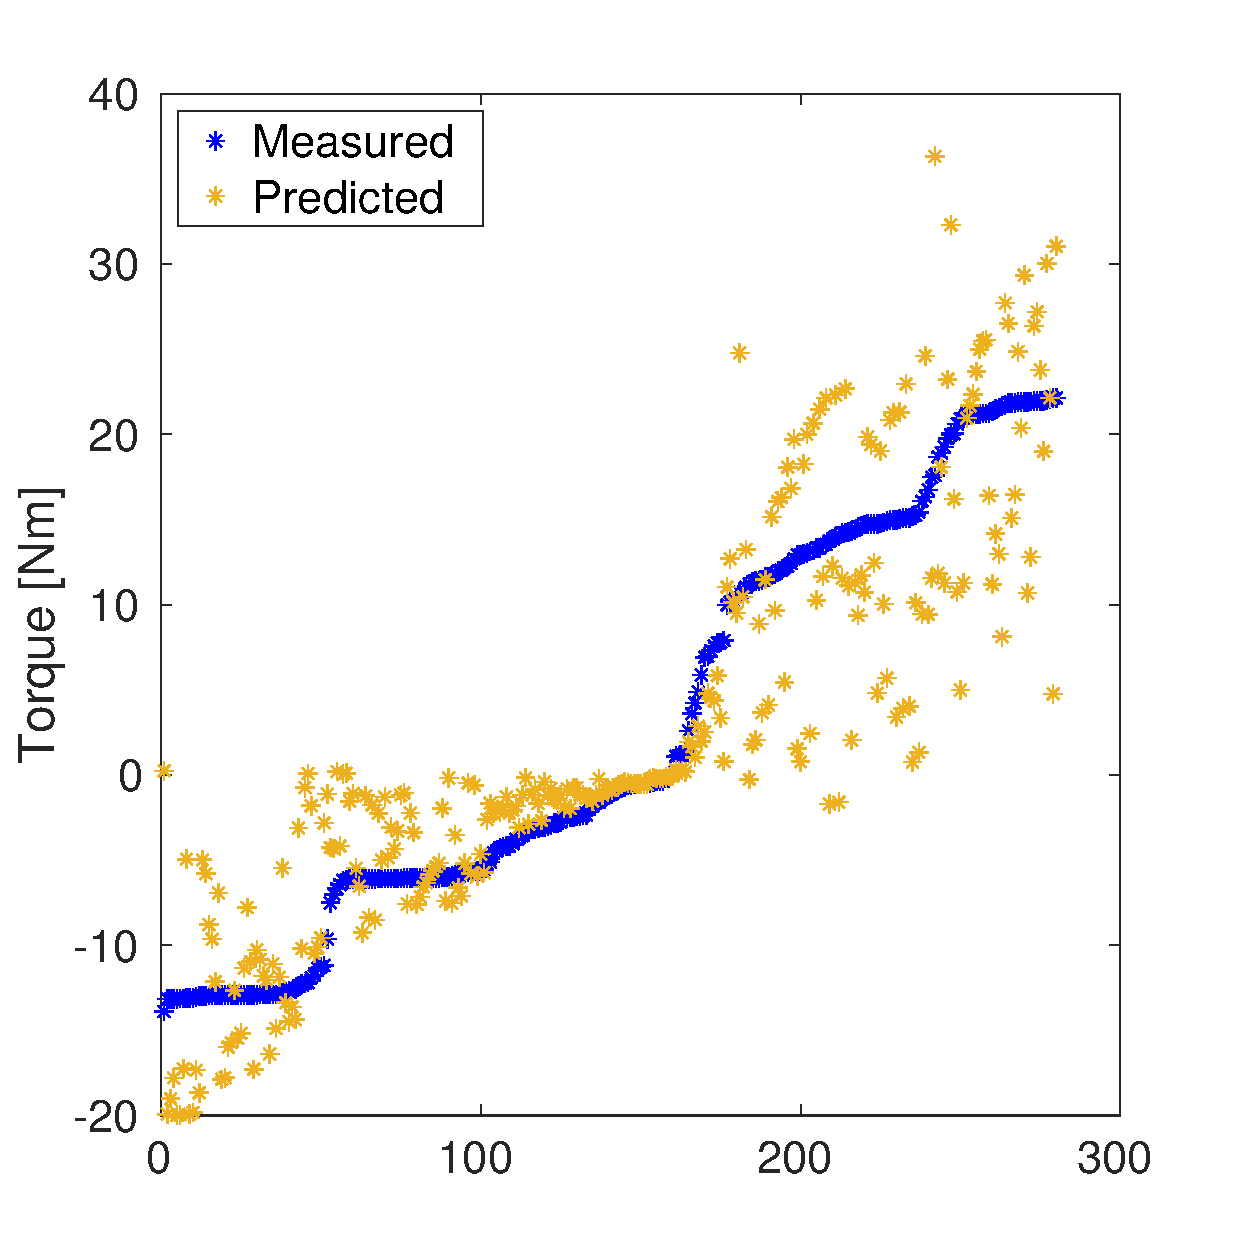
\includegraphics[width=\textwidth]{images/summer_school_study/measured_optimized_torque_B.pdf}%
    \caption{Measured values (blue) and values predicted by model B (orange).}%
    \label{fig:measured_optimized_torque_B}%
  \end{subfigure}%
  \caption{Resubstitution prediction: Measured and predicted torque values for the training data set. The measured points are ordered and numbered by magnitude, the order of the predicted points matches the order of the measured points.}%
  \label{fig:measured_optimized_torque}%
\end{figure}%

\subsection{Validation}\label{sec:res_validation}

The next evaluation uses the validation dataset and compares the predicted outputs of the models with the actual experimental values.
In contrast to the training data, where a small number $n$ of points was selected, we now use all captured values. This involves a total of \num{54e3} data points for a time span of $t=\SI{54}s$. 

\begin{figure}%
  \centering%
  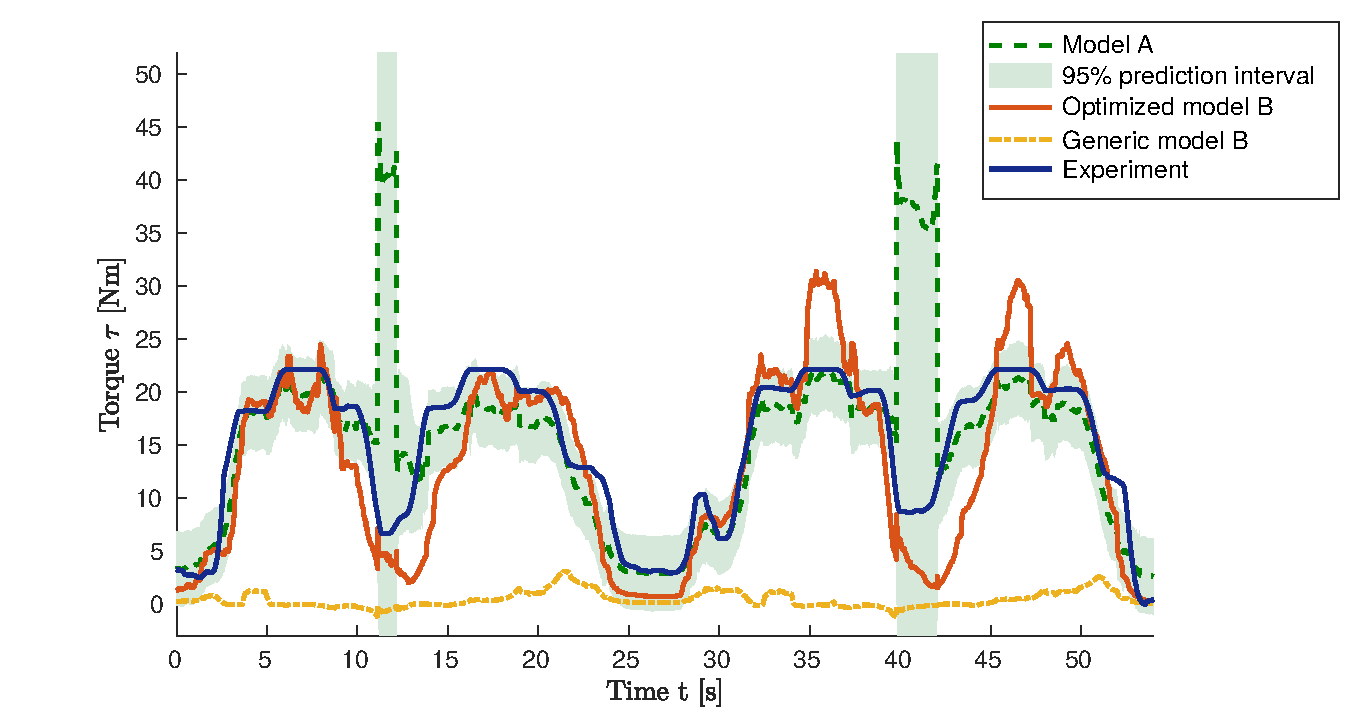
\includegraphics[width=\textwidth]{images/summer_school_study/validation_bv5_40_points.pdf}%
  \caption{Validation: Predicted torque values by model A (green), trained model B (red) and untrained model B (yellow), in comparison to the experimentally measured values (blue), for the validation data set.}%
  \label{fig:validation_bv5_40_points}%
\end{figure}%

The results are shown in \cref{fig:validation_bv5_40_points}. Comparing the green curve for model A with the blue curve for the experimental data, it can be seen that the predicted values match qualitatively for most of the time span. The predicted torque values appear consistently slightly smaller than the real values. Only for the two intervals $[\SI{11}s, \SI{12}s]$ and $[\SI{40}s, \SI{42}s]$ the predicted value is far off. The \SI{95}\percent{} confidence interval that was computed by the Gaussian Process spans a large range for these time intervals which implies that the model prediction is not to be trusted for this area. 

The biophysical model approach, model B, was tested in two variants. First, with the generic parameters from literature (yellow curve), second, with the subject-specific, optimized parameters (red curve). It can be seen that the generic model fails to predict the torque values whereas the trained model predicts reasonable values. These values are worse than most of the predictions from model A, but they succeed in giving a qualitative estimate about a low, medium or high torque output.

The match between model outputs $\tau_i$ and experimental data $\hat\tau_i$ can be quantified using the normalized root-mean-square error (NRMSE). This is a scaled version of the root-mean-square error (RMSE) and can be defined as
\begin{equation*}
  \begin{array}{lll}
    \text{RMSE} = \sqrt{\sum\limits_{i=1}^N (\tau_i - \hat{\tau_i})^2 / N},\\[4mm]
    \text{NRMSE} = \dfrac{\text{RMSE}}{\max\limits_i\{\hat\tau_i\} - \min\limits_i\{\hat\tau_i\}}.
  \end{array}
\end{equation*}
The NRMSE for model A is 0.267 which is worse than the value of 0.163 for the trained model B. The generic model B has the worst NRMSE of 0.547.

\subsection{Simplified Model A}\label{sec:res_simplified_a}
An advantage of model approach A is that it forgoes any biophysical description and the associated type of model error. It is a generic approach that does not require expert knowledge about the physiological structure. In the present study, however, some level of expert knowledge and physiological model was required in preprocessing the MoCap data, i.e. solving the inverse kinematics of the observed forearm movements to get the kinematic quantities of muscle lengths, velocities and moment arms. 

Since model A performed well in the previous validation study, we tested whether good results can also be achieved without this expert knowledge.
Consequently, the next study applies model approach A using only the elbow angle and no muscle lengths, velocities nor moment arms. Thus, the training data consists of input vectors $\bfx_i = (\phi_e(t_i), \gamma_B(t_i), \gamma_T(t_i))^\top \in \mathcal{X}$. In the following, this model is named \say{simplified model A} in contrast to the \say{full model A} that uses the complete set of input variables.

The results are shown in \cref{fig:measured_optimized_A2}. It can be seen that the resubstitution prediction in \cref{fig:measured_optimized_torque_A2} where the trained model is used to predict the training values shows a perfect fit. In contrast to the full model A, \cref{fig:measured_optimized_torque_A}, here, the learned input-output mapping shows no variance. However, the prediction for the validation dataset in \cref{fig:measured_optimized_torque_A3} shows a high error relative to the experimental data. The curve for the experimental data even lies outside the 95\% confidence interval of the prediction at some points. 

The simplified model A has a NRMSE value of 0.461. For comparison, the NRMSE values of the full and simplified model A and the generic and optimized model B are summarized in \cref{fig:nrmse}. 

This evaluation shows that simplified model A gives no useful results where the training input is too scarce. Instead, preprocessing of the measurements using a subject specific geometric model, as done for the full model A, is needed to allow for a useful prediction.

\begin{figure}%
  \centering%
  \begin{subfigure}[t]{0.48\textwidth}%
    \centering%
    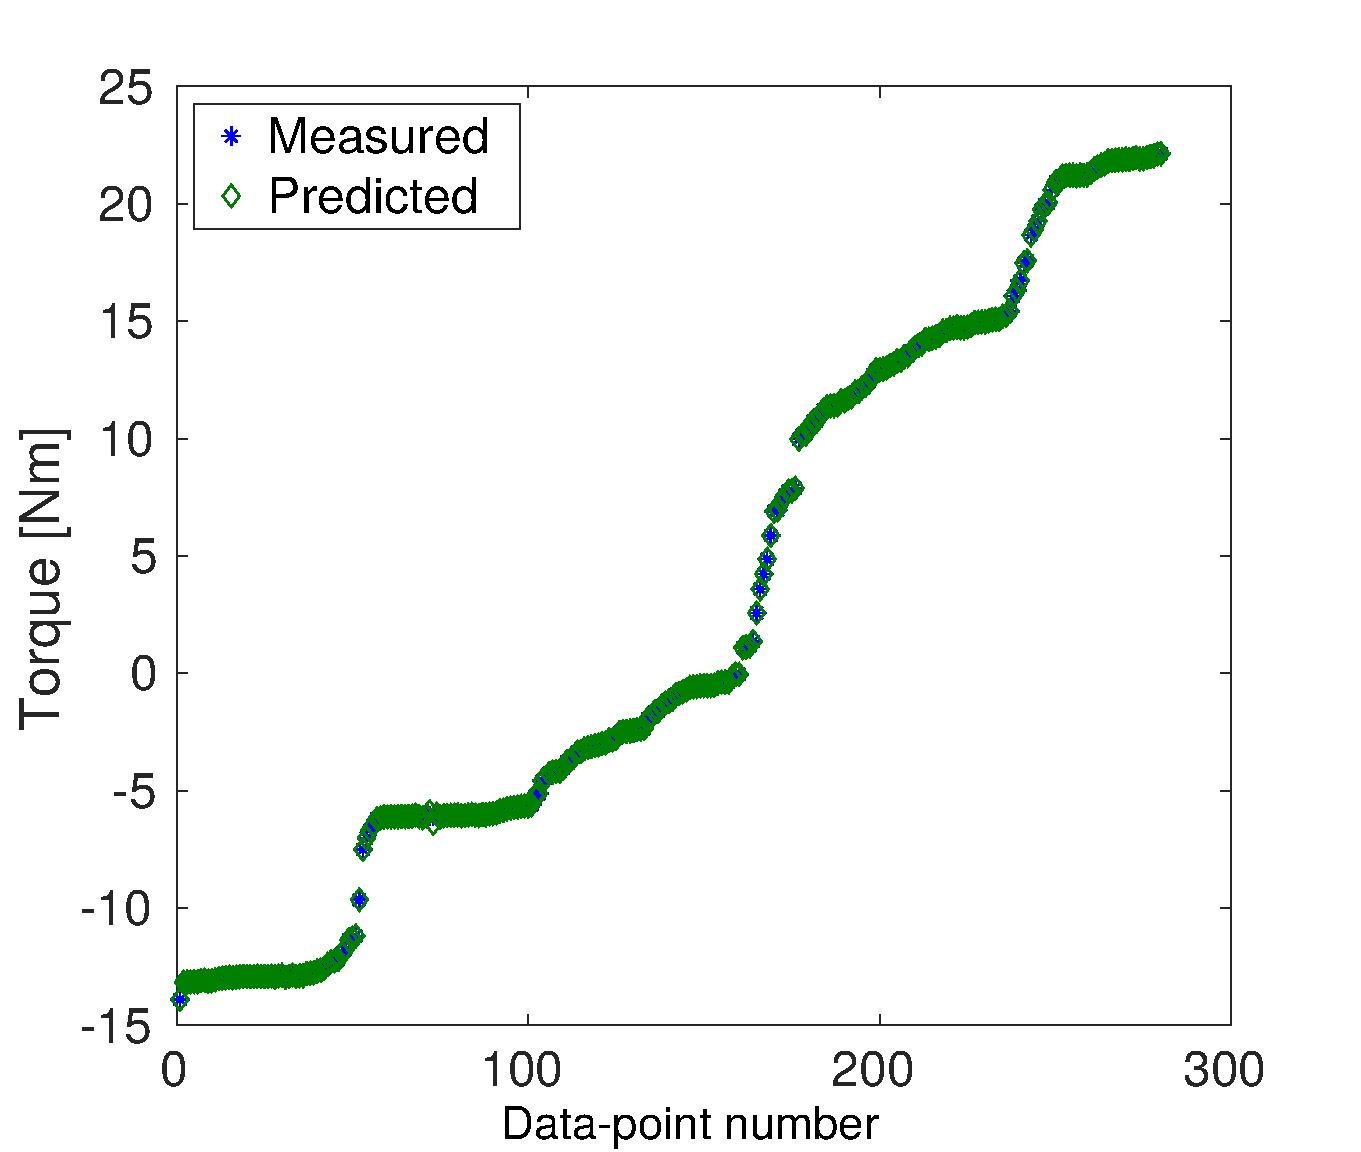
\includegraphics[width=\textwidth]{images/summer_school_study/measured_optimized_torque_A2.pdf}%
    \caption{Measured and predicted torque values of the training dataset, ordered and numbered by magnitude. The measured values (blue) and the values predicted by the Gaussian Process (green) lie on each other.}%
    \label{fig:measured_optimized_torque_A2}%
  \end{subfigure}%
  \quad
  \begin{subfigure}[t]{0.48\textwidth}%
    \centering%
    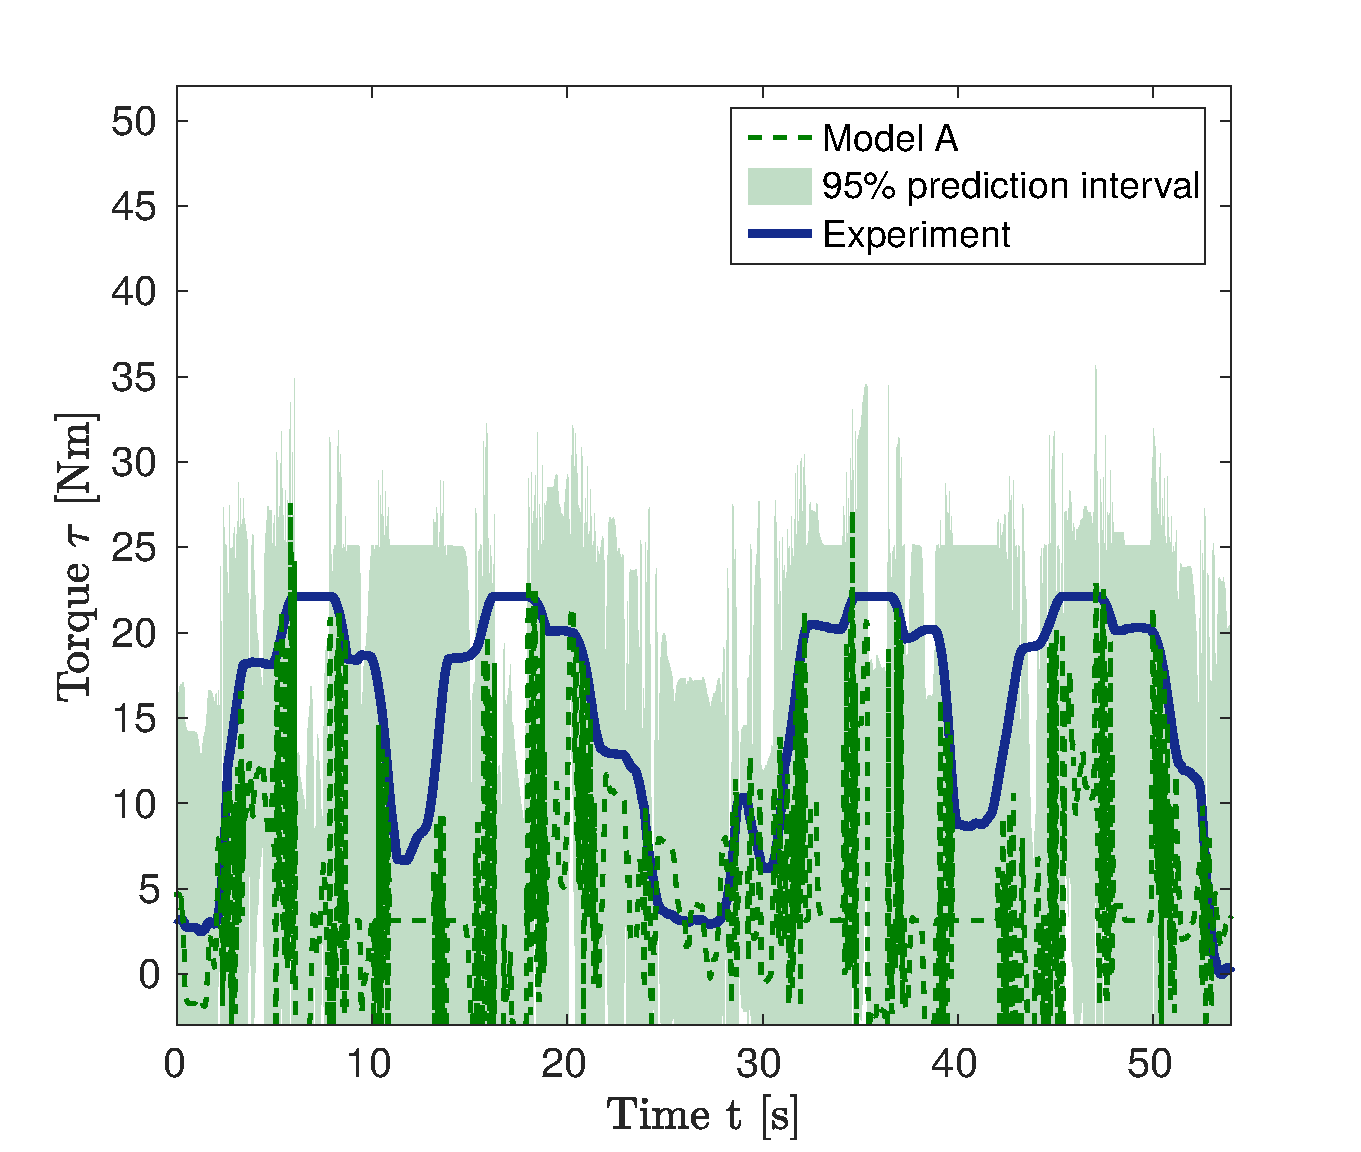
\includegraphics[width=\textwidth]{images/summer_school_study/validation_bv5_40_points_only_gamma_for_training.pdf}%
    \caption{Predicted torque values for the validation trials (green dotted line), 95\% confidence interval (light green) and the reference values of the experiment (blue). The plot reveals bad prediction capabilities of the simplified model A.}%
    \label{fig:measured_optimized_torque_A3}%
  \end{subfigure}%
  \caption{Result for the simplified model A, where, apart from the free calcium ion contractions, only the elbow angles, $\phi_e$, are used as training input instead of MTU lengths, velocities and moment arms.}
  \label{fig:measured_optimized_A2}%
\end{figure}%

\subsection{Insights of Model B}\label{ref:res_insights_b}
An advantage of model approach B is that the trained parameters are physically meaningful and allow insight into the properties of the subject specific model. Furthermore, the quality of the training data can be assessed. \Cref{fig:biceps_working_area} shows the force-length relation of the biceps muscle model using the generic and the optimized parameter values. It can be seen that the subject-specific model has a smaller slope of the force curve. 
All points of the training data set are indicated by red crosses on the curves and show the operating range of the muscle in which the model has been trained. It can be seen that the experimental training data are limited to a small range of the muscle length below its optimal CE length $l_{\CE,\text{opt}}$. In order to improve the quality of the model predictions for this subject, specific additional experimental trials can be designed for model training. They can be designed to fill in values in the missing range of operation, which in this case is for larger muscle extensions.

A low computational time of the offline parameter identification and the online evaluation of the two models would be an important measure for their practical applicability. In the present study, the training phase of Model A, i.e., optimization of the quantities for the Gaussian Process Regression using 280 training data points took \SI{2.24}{\second}. The evaluation of Model A for the validation data set containing \num{54e3} points had a duration of \SI{116}{\milli\second}.

The runtimes for model B were significantly higher. The parameter optimization lasted \SI{25}{\minute} \SI{16}{\second} and the evaluation for the validation data set had a duration of \SI{13}{\second}.

The large differences in runtime between models A and B can be explained by the inefficient implementation of the biophysical model using the MATLAB programming language. During parameter identification, this model needs to be evaluated iteratively in the optimization algorithm. In contrast, the optimization within model A works with an internal implementation of the Gaussian Process which was optimized during development of the particular MATLAB functionality.
In general, the evaluation of Gaussian Process Regression has cubic time complexity whereas, for the parameter optimization of model B, iterative solvers with linear time complexity exist.

\begin{figure}%
  \centering%
  \begin{subfigure}[t]{0.47\textwidth}%
    \centering%
    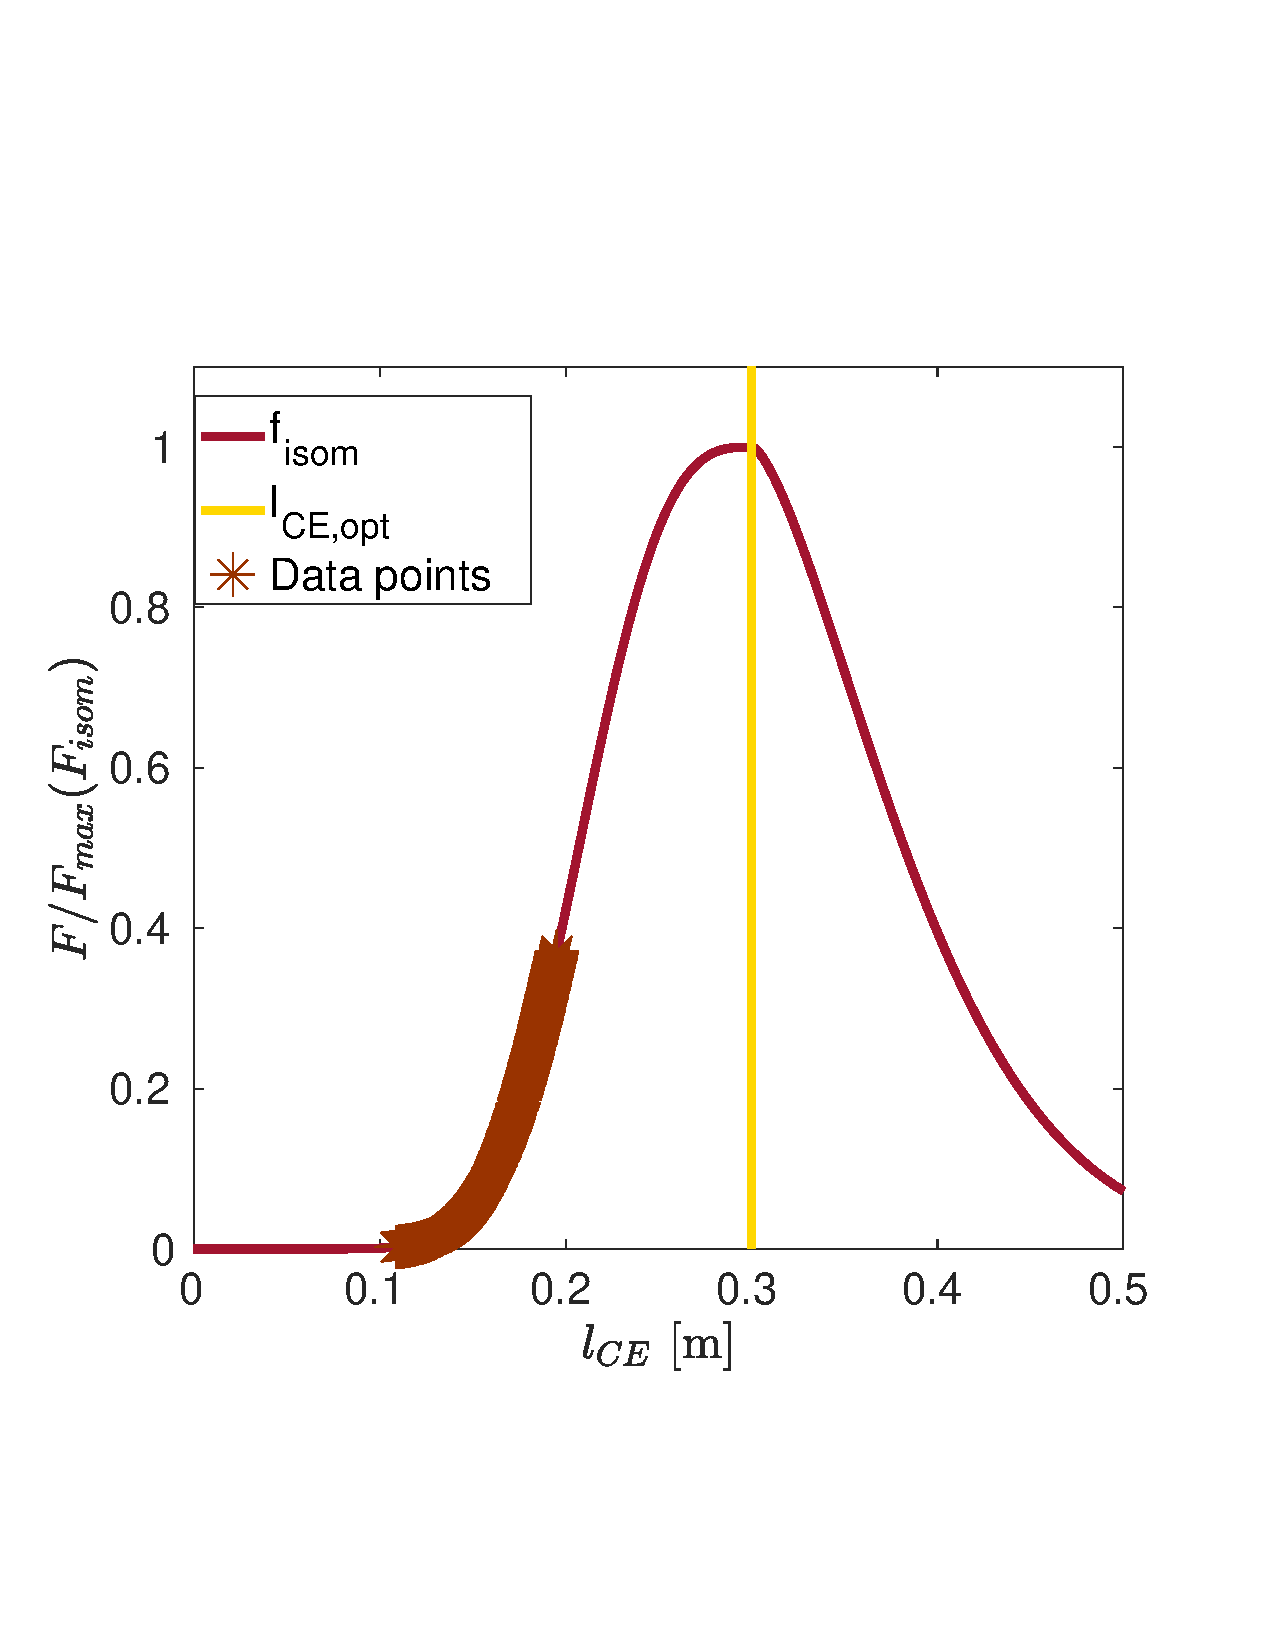
\includegraphics[width=\textwidth]{images/summer_school_study/biceps_initial.pdf}%
    \caption{Model with generic parametrization.}%
    \label{fig:biceps_a}%
  \end{subfigure}%
  \quad
  \begin{subfigure}[t]{0.47\textwidth}%
    \centering%
    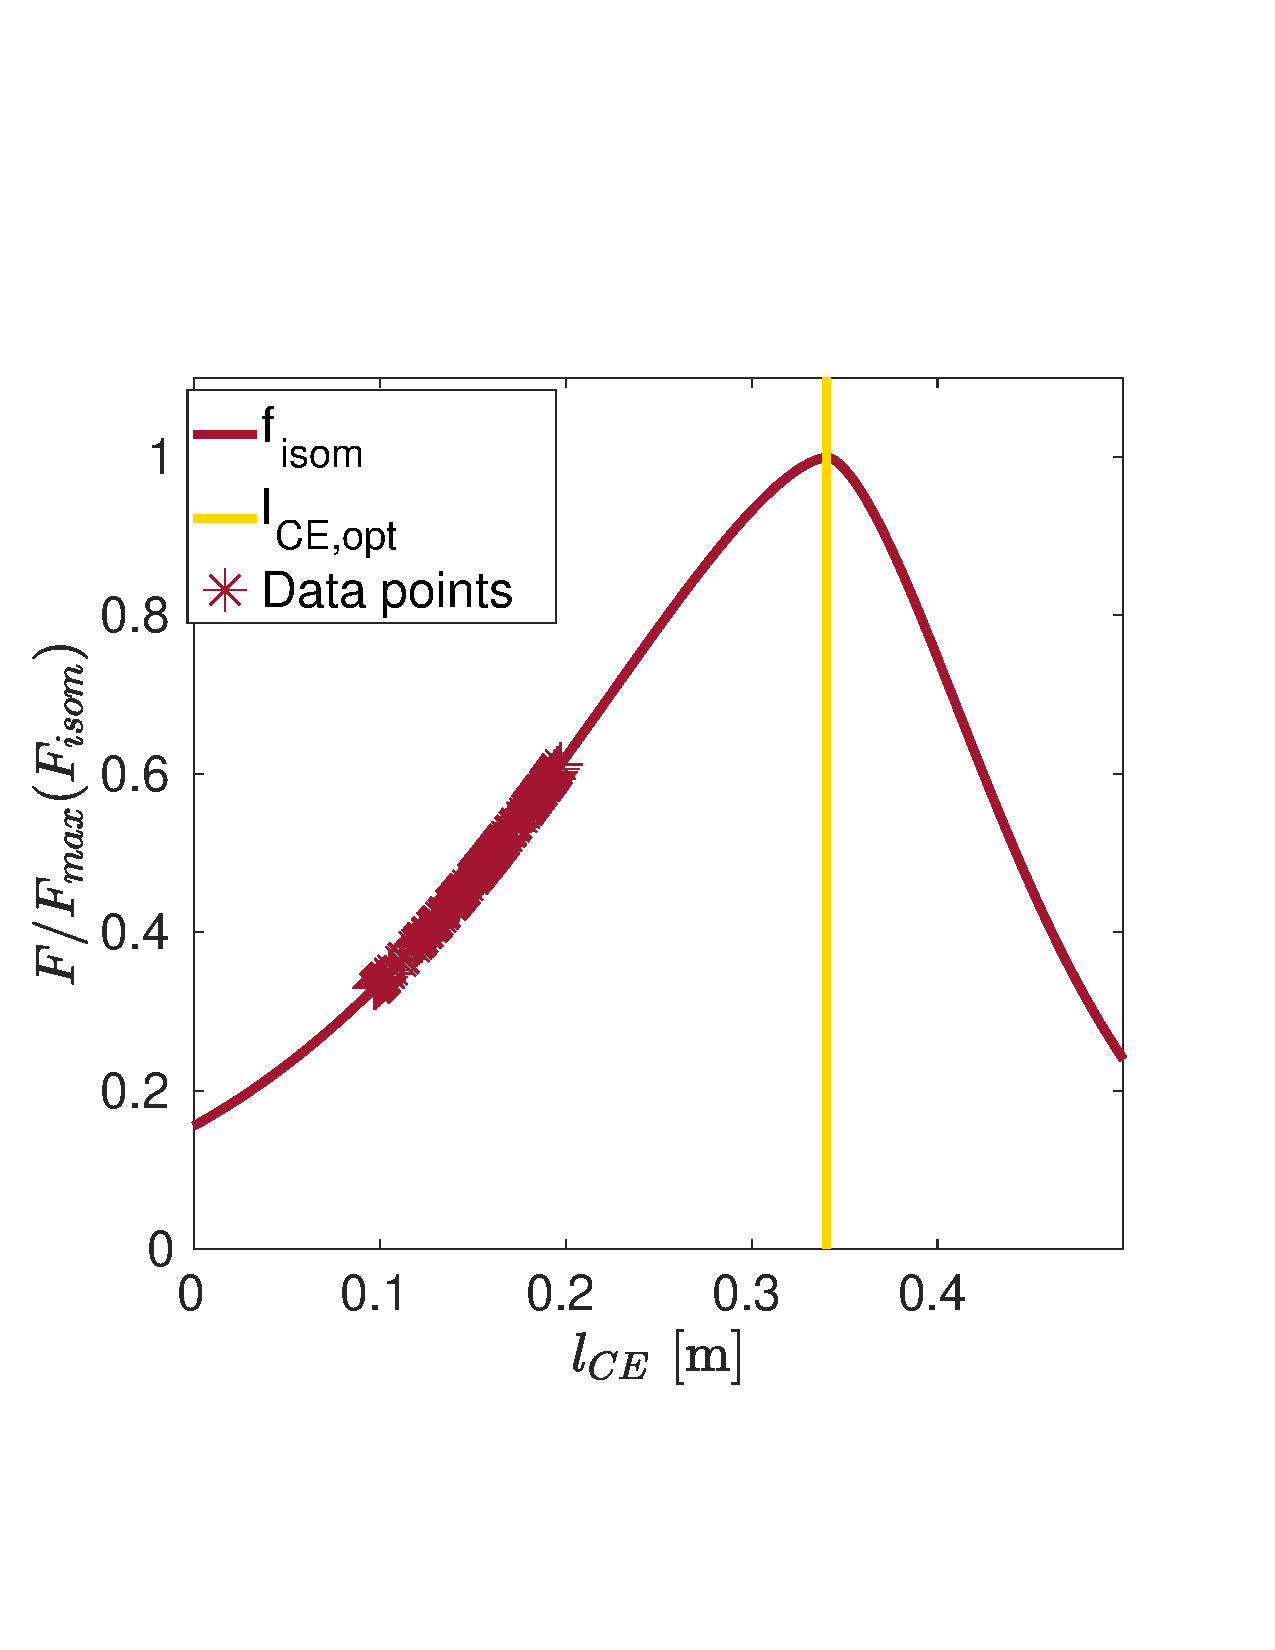
\includegraphics[width=\textwidth]{images/summer_school_study/biceps_optimized.pdf}%
    \caption{Model with subject-specific parametrization.}%
    \label{fig:biceps_b}%
  \end{subfigure}%
  \caption{Isometric force-length relation of the CE for the biceps model, analogue to \cref{fig:force_curves_generic_length}, but additionally with training data points. The points are placed on the model curve and visualize the predicted relative forces for the lengths of the CE that occurred during the training trials.}%
  \label{fig:biceps_working_area}%
\end{figure}%


\begin{figure}%
  \centering%
  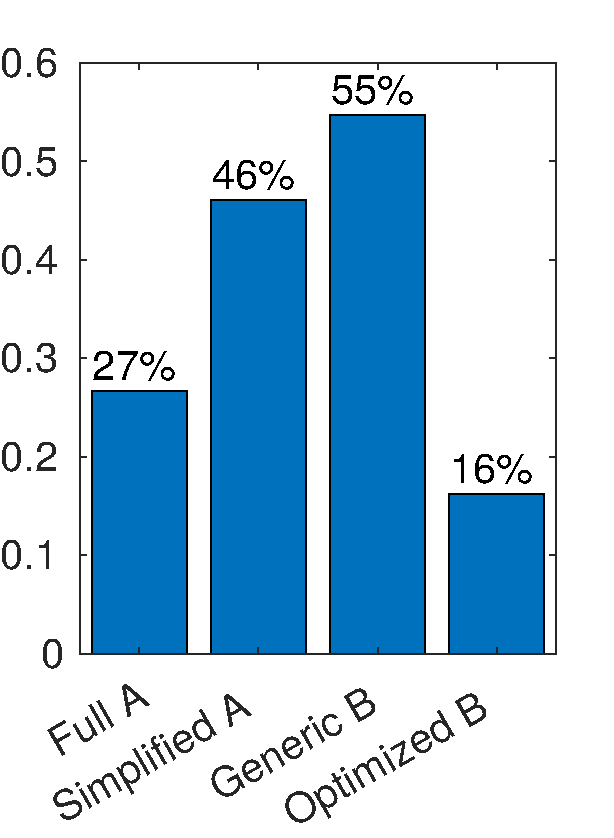
\includegraphics[width=0.35\textwidth]{images/summer_school_study/nrmse.pdf}%
  \caption{Normalized Root Mean Square errors (NRMSE) of the validation trials between the respective models and the measured values. A lower error value means a better fit.}%
  \label{fig:nrmse}%
\end{figure}%

\section{Conclusion}\label{sec:study_conclusion}
In this study, elbow torques during flexion and extension of the upper arm were predicted from motion capture data and EMG measurements. Two models, A and B, were developed. Model A is non-parametric and uses Gaussian Process Regression. Model B is biophysically informed and involves two state-of-the-art Hill-type muscle models for biceps and triceps. Experiments were conducted to generate training and validation data. These training data were used for model parameter identification. Predictions from the two models were compared to real experimental values using the validation data.

Regarding the formulation and implementation, model A requires low effort and no special knowledge about the model, except where experimental motion data is preprocessed for a specific subject. In contrast, model B needs expert knowledge about the biophysical structure and the implementation of all comprised models.

Similar holds for the offline training phase. There are no parameters in model A that have to be tuned manually, which allows a quick start. Conversely, model B requires the appropriate definition of initial values and physiological constraints for the optimization problem. However, this can also be seen as an advantage for model B, as a-priori knowledge can be integrated in such a model.

On the other hand, an advantage of model A is that additional experimental data, e.g., from neighboring muscles or additional sensors, can easily be added to the model. This is not possible with model B, where the model formulation would have to be changed.

Our studies showed that both models were able to predict the levels of torque reasonably. 
\Cref{fig:nrmse} showed the best score for model A, followed by model B. It was also seen that the generic parametrization of model B does not yield a useful prediction. The same is true for a simplified version of model A, where the elbow torque was used as training input instead of derived quantities from the motion capture system that required a complex preprocessing step.

Both models provide possibilities to assess the confidence of their predictions. With model A, confidence intervals can be computed directly from the Gaussian Processes. Their usefulness was shown in the validation where regions with large errors also had a large confidence interval. 
Model B allows insight into force-length and force-velocity characteristics of the two involved muscles. The operating ranges of the muscles during the experiments can be visualized and allow assessing whether the desired model features were covered by the training phase and, thus, will yield a good prediction.

In our study, runtimes were low for model A and high for model B in both offline and online phases. However, this is due to our prototypical implementation of model B. For larger data sizes and a more sophisticated implementation, the reverse effect is expected. The runtime complexity for the training phase is better for model B (linear in time) compared to model A (cubic in time). For the online phase, costly integration over data points is needed for model A whereas model B directly provides a differential equation of the system that can be solved efficiently. 

If EMG is used to control an exoskeleton that supports the movement of the limb, it is known that the measured signals are ahead of the intended movement by a small offset. This is a result of the time delay in the neuromusculoskeletal system. This property gives the assistive exoskeleton a short time to predict the intended movement and thereby allows a seamless integration of the artificial device with human control.

When targeted at such a real-time application, both models could be considered to be integrated into the control. Model A better fits the use case of a device that could be (re\nobreakdash-)calibrated by the patient itself. Because of the built-in estimation of prediction quality, compliance and safety could be ensured more easily even for imperfect training.
Model B would need a controlled environment such as a specialist's laboratory and careful assistance for the calibration process.
After calibration, it would promise a more natural and more responsive experience because of the subject-specific model and possibly smaller compute times.

Where real-time application is not a requirement, biophysically informed models have a high potential to leverage the understanding how the human neuromusculoskeletal system operates for given tasks.
In model B of this study, the kinematics and individual muscle dynamics were described close to the current  understanding of the system. However, several aspects where not modeled as detailed as possible. The pathway from neural stimulation to excitation and activation of the muscle, the recruitment strategies including different motor units, neural feedback loops as well as effects stemming from the 3D geometry of the muscle were not considered. Therefore, this thesis develops a more detailed, biophysically informed model including these properties in the following chapters.

The presented study reproduced what similar studies in literature have shown: Subject-specific model identification for Hill-based torque prediction models can vastly improve the prediction quality compared to generic models. Our work adds to the common knowledge that this holds also for the four-element Hill-type model that was used for model B. Furthermore, a comparison with Gaussian Process Regression was given, various advantages and disadvantages of these two approaches were identified. Future work can test the two models with more subjects and increase the variety of motion in the training experiments. For example, effects resulting from high contraction velocities or eccentric contractions could be investigated to evaluate the model's potential in more complex movements.


\chapter{Muscle Fibers and Motor Units} 
The activation of muscle fibers is governed by the functional organization of the fibers in motor units (MU). An MU is the set of fibers that are innervated by the same $\alpha$-motor neuron, together with the neuron. If a motor neuron fires, all muscle fibers within the MU are activated. The association of the muscle fibers with MUs needs to be specified for electrophysiology simulations that consider activated muscle fibers. This chapter describes algorithms to achieve an MU-fiber association based on biophysical principles.

\section{Introduction}\label{sec:mu_intro}
Given a number of muscle fibers, the goal is to assign each fiber to one MU out of a set of given MUs. A muscle with a fusiform geometry, such as the biceps brachii is considered. Because muscle fibers do not branch or interrupt within the belly of such a muscle, the task can be reduced to the 2D problem on a cross-section of the muscle.

Properties of MUs have been subject to various investigations in literature. The number of MUs in a human muscle can be estimated by anatomical and physiological methods \cite{MacIntosh2006}. Anatomical methods include counting large-diameter fibers in post mortem tissue. The morphologic studies of \cite{Feinstein1955} revealed high variations between different muscles. For example, the brachioradialis muscle has an estimated number of \num{333} MUs with \num{410} muscle fibers on average whereas the external rectus muscles in the eye have \num{2970} MUs with an average of only 9 muscle fibers. 

Physiological methods involve comparing the electrical and mechanical responses of artifically activated muscles, e.g., as in \cite{Milner-Brown1973b,Thomas1990b}. Typically, a high number of MUs with a smaller force or electric response is observed and a smaller number of MUs with a higher response. 
The review of \cite{Enoka2001} collects available experimental results and concludes an exponential distribution of the number of fibers per MU over all the MUs in a muscle.
% Enoka and Fuglevand (2001): Motor unit physiology: some unresolved issues

The spatial arrangement of the fibers of an MU can be revealed by a histochemical method \cite{brandstater1969histochemical}. It was found that the fibers of an MU appear at random positions but are grouped in a sub region of the muscular cross section. The size of the sub region varies among muscles and fiber types and can be as large as one quarter of the cross section, as in the tibialis anterior of the rat \cite{Edstrom1968}. Although the fibers of an MU are located in proximity they usually do not touch each other, i.e., there are always fibers of other MUs in between the fibers associated with an MU.

In our algorithm for assigning fibers to MUs we incorporate the following properties that are founded on biophysical experiments. 
\begin{itemize}
\item[(a)] The number of fibers per MU is  exponentially distributed. 
\item[(b)] The fibers of an MU are spatially distributed around a center point of the MU territory.
\item[(c)] The MU center points are reasonably separated from each other. However, the MU territories intermingle. 
\item[(d)] The spatial extents of the MU territories are proportional to the number of fibers of the MUs. 
\item[(e)] The exact locations of the fibers are random, but the overall density of fibers in the muscle is approximately constant. 
\item[(f)] Neighbouring fibers are not innervated by the same motor neuron and therefore belong to different MUs.
\end{itemize}

Further physiological properties of fibers such as their fast or slow-twitch type as well as the distribution of electrical and mechanical properties are not subject to the fiber assignment algorithm. They are considered during configuration of the simulations of electrophysiology or muscular contraction.

\subsection{Related Works}
Simulations involving individually resolved muscle fibers are scarce in the literature. Therefore, not much previous work exists regarding methods to algorithmically assign fibers to MUs. The chemo-electro-mechanical skeletal muscle framework of \cite{Heidlauf2013} uses a method introduced in \cite{Roehrle2012} where center points of MU territories are positioned normally distributed around two distinct weighting centers for fast- and slow-twitch fibers. 
The algorithm randomly selects from certain sets of fibers and assigns them to MUs with exponentially increasing MU sizes. 
%\sout{However, the formulation contains mathematical inaccuracies and therefore the process of the exact algorithm can only be guessed.} 
The method is applied to determine up to 50 MUs in the tibialis anterior (TA) muscle.

This algorithm fulfills the previously formulated properties (a)-(e). Among those, the fulfillment of (c) is not guaranteed but may be given by the random nature of the algorithm. An assumed issue regarding property (b) is that no predictions can be made about the fiber locations of the larger MUs. The larger MUs get assigned to previously unassigned fibers in a late stage of the algorithm, after most of the fibers have been selected for smaller MUs. The largest MU simply gets associated with all remaining fibers that were not selected for other MUs. In the worst case, these fibers can accumulate at multiple different regions, e.g., at boundaries of the muscle which is not physiological.

Instead of the 3D setting in \cite{Roehrle2012} that was needed for the complex anatomy of the TA muscle, we restrict our problem to a 2D cross-section of a fusiform muscle such as the biceps brachii. In comparison, our method creates MU territories of equal quality for all MUs and additionally fulfills property (e). Slow- and fast-twitch fibers are not treated differently by our algorithm, their properties are considered later in the simulation settings.

3D Simulations of skeletal muscle exist that treat MU association as homogenized property in the muscle volume. The approach in \cite{harry2018} assigns volume fractions of MUs to every spatial point of a 3D FEM discretization grid. MU center points are selected randomly ensuring a minimal distance. Prescribed volume fractions are sequentially assigned for each MU. The degree of intermingling can be adjusted by a parameter. It is shown that the algorithm highly depends on the order in which the MUs are traversed. The algorithm fulfills the properties (b)-(e), fulfilling (a) is possible by using appropriate parameter values.

In comparison, our method is targeted at MU assignment to individual fibers. However, distributing volume fractions is also the first step in our method. The volume fractions are interpreted as probabilities of the fibers being assigned to the respective MU. Therefore, our method can also be used as generator for homogenized formulations. A difference is that our method does not depend on a traversing order of MUs and ensures the exponential distribution of MU sizes.

\subsection{Two Alternative Premises for Motor Unit Assignment}
% Röhrle2012: TA 12 elements, MU association
% Heidlauf2013: 400 fibers, TA, OpenCMISS, mechanics

We identify two different sets of requirements which lead to two different methods.
Both methods fulfill the properties (a)-(f) listed in \cref{sec:mu_intro}.
The first premise is to assign motor units to a given number of fibers such that every fiber is associated with one MU. The second, alternative premise is to assign motor units only to a portion of the given set of fibers, discarding unassigned ones and thereby reducing the resulting set of fibers.

With the first setup, simulations of muscles that are gradually activated by motor neurons are possible. Activating the full muscle corresponds to activating all MUs and, in consequence, all muscle fibers. In reality, it is hardly possible to voluntarily activate all fibers in a muscle. This approach is also chosen in the presented literature, \cite{Roehrle2012} and \cite{harry2018}.

The second setup corresponds to modeling only a part of the muscle. The discarded fibers can be seen as belonging to other MUs that are not part of the simulation. When running highly parallelized simulations containing a large number of fibers, the missing fibers can introduce load imbalances, if they are computationally treated equally to the fibers with MUs. Even if no extra computational time is spent for the discarded fibers, a parallel domain decomposition becomes more involved than with the first setup where all fibers in a grid are present.

An advantage of the second setup is that the MU assignment to the fibers is generally easier. It also has its analogue in volume fraction methods, where scalar fields of factors $f_k: \Omega \subset \R^3 \to [0,1]$ representing multiple MU territories, $k=1, \dots, n_\text{MU}$, can be easily defined. With this setup it is possible, for example, to perform analogous EMG simulations with the Multidomain model of \cite{Klotz2020} and the fiber based model of \cite{Mordhorst2015}.

In the remainder of this chapter, \cref{sec:method1_assignment} presents method 1, which fulfills the first premise where all fibers are associated to the MUs. Next, \cref{sec:method2_selection} introduces method 2, which only associates some fibers to MUs. Methods 1 and 2 fulfill the properties (a)-(e). Two derived methods 1a and 2a are subsequently constructed in order to also fulfill property (f). They are presented in \cref{sec:method3_modification}. Results and a discussion is given in \cref{sec:mu_results_and_discussion} before the chapter ends with a conclusion in \cref{sec:mu_conclusion}.

\section{Method 1: Assignment of Motor Units to a Given Set of Fibers}\label{sec:method1_assignment}

In our methods to assign MUs to muscle fibers, the considered set of muscle fibers is organized in a regular grid. \Cref{fig:mu_grid0} shows 
a part of the cross section of a skeletal muscle, the domains of individual fibers are visible. \Cref{fig:mu_grid1} visualizes the representation of muscle fibers in our simulations. In this figure, a relatively low number of 49 fibers was modeled. The fibers are approximated by 1D lines with uniform spacing in radial direction. For the algorithms to assign MUs to fibers, the muscle cross section is considered as a logical 2D grid with a quadratic number of $n \times n$ fibers. Such a grid is visualized in \cref{fig:mu_grid2}.

\begin{figure}%
  \centering%
  \begin{subfigure}[t]{0.32\textwidth}%
    \centering%
    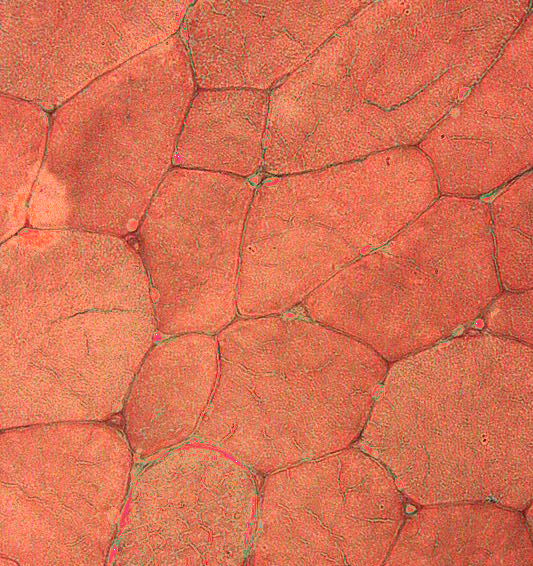
\includegraphics[width=\textwidth]{images/motor_unit_assignment/mus1.png}%
    \caption{Muscle fibers in the cross section of a muscle visualized by Gömöri trichrome stain\footnotemark}%
    \label{fig:mu_grid0}%
  \end{subfigure}
  \quad
  \begin{subfigure}[t]{0.28\textwidth}%
    \centering%
    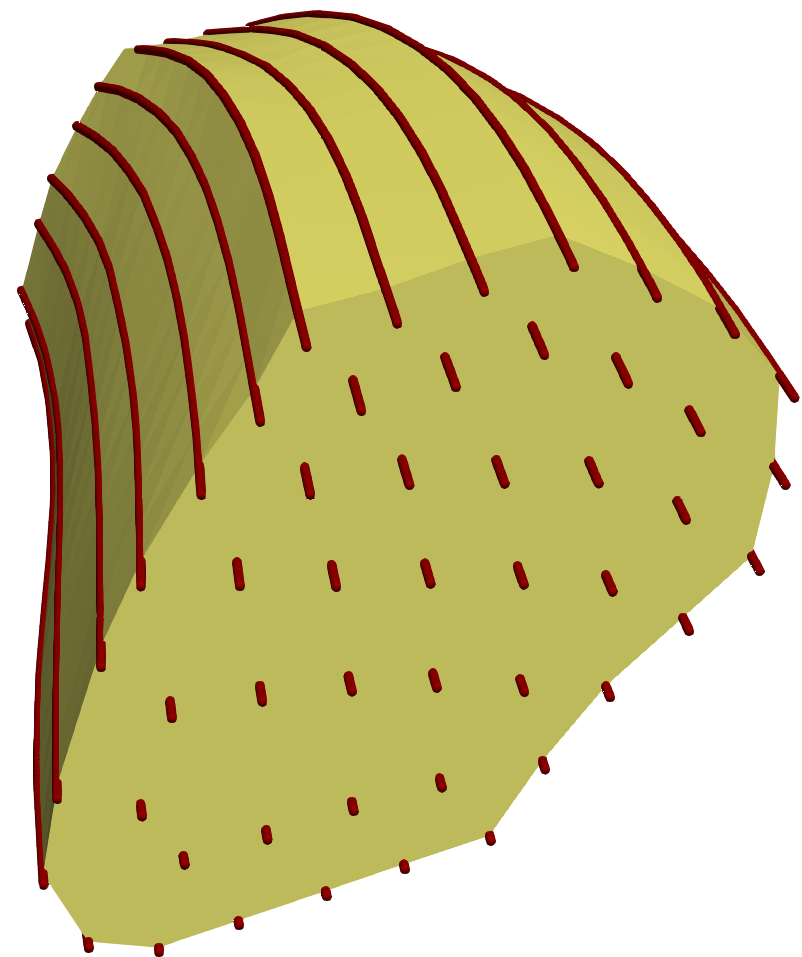
\includegraphics[width=\textwidth]{images/motor_unit_assignment/muscle_mesh_fibers.png}%
    \caption{A cut open muscle with $49$ muscle fibers in the simulation domain}%
    \label{fig:mu_grid1}%
  \end{subfigure}
  \quad
  \begin{subfigure}[t]{0.33\textwidth}%
    \centering%
    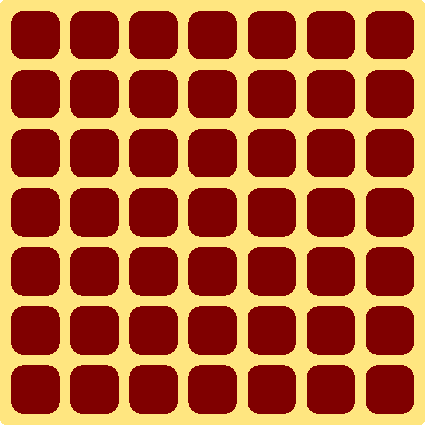
\includegraphics[width=\textwidth]{images/motor_unit_assignment/muscle_fibers_grid.pdf}%
    \caption{A quadratic grid of $7 \times 7$ fibers, used for the methods to assign MUs to fibers.}%
    \label{fig:mu_grid2}%
  \end{subfigure}
  \caption{Representation of muscle fibers for the methods to associate fibers with MUs: From the real muscle to a quadratic grid.}%
  \label{fig:mu_grid}%
\end{figure}%

\footnotetext{Image copyright © 25/12/2010 Michael Bonert (\url{https://commons.wikimedia.org/wiki/User:Nephron}), CC BY-SA 3.0 (\url{https://creativecommons.org/licenses/by-sa/3.0/legalcode}). The picture shows mitochondrial myopathy, it was cropped and the color was adjusted to make the \say{ragged red fibers} less prominent.}
\stepcounter{footnote}


The first method for the assignment of MUs to a given set of fibers associates the $n \times n$ fibers to a set of $n_\text{MU}$ motor units.
First, for each fiber ${(i,j)}$ in the grid, the probabilities $p(i,j,k_\text{MU})$ to be assigned to MU $k_\text{MU}$ are computed. This computation involves the solution of an optimization problem. Second, the sampling step assigns the actual MU indices to the fibers.

\subsection{Stochastic Formulation of Motor Unit Assignment}\label{sec:stochastic_formulation_and_algorithm}

In order to fulfill the formulated properties, the following three conditions are enforced on the probabilities. 
\begin{itemize}
\item[(i)] The probabilities at every fiber  have to be valid, i.e., positive and sum up to 1 for all MUs.
\item[(ii)] The portions fibers associated to MUs have to approximately follow an exponential progression $q$, with MU 1 containing the least and MU $n_\text{MU}$ containing the most fibers.
\item[(iii)] For any given MU, the spatial arrangement of its fibers in the cross-sectional plane is described by a radial kernel function $\hat{p}$. The fiber density of the MU increases when moving closer to the center point of the MU. This condition approximates the fact that the fibers of an MU are located in proximity, forming the MU territory.
\end{itemize}

The exponential progression $q$ in condition (ii) is defined as follows,
%
\begin{align}\label{eq:mus_q}
  q(k_\text{MU}) = b^{k_\text{MU}} / \s{\ell=1}{n_\text{MU}} b^\ell.
\end{align}
%
% f(x) = 1/(1+a*x^2),  ∫f(x)dx = arctan(sqrt(x)*x)/sqrt(a) + c
% stddev = sqrt(variance) = sqrt(∫{-∞,+∞} (f(x)-0)^2 dx) = sqrt(pi/(2*sqrt(a)))
% => a = pi^2 / (4*\sigma^4)
%
% 
The basis $b$ is a parameter and should be set to a value greater than one, e.g., $b=\num{1.2}$. \Cite{Enoka2001} formulate the function to be proportional to $\exp(\log(R)/n_\text{MU}\cdot k_\text{MU})$ where $R$ is the constant ratio between the sizes of the largest and smallest MUs. Our form is equivalent with $b = R^{1/n_\text{MU}}$.

The value of $q$ in \cref{eq:mus_q} is always positive. The division by the scaling factor ensures that the probabilities for all MUs sum up to one. Thus, condition (i) is fulfilled. The construction with the exponential function fulfills condition (ii).

For condition (iii), center positions $\bfx_{k_\text{MU}}, k_\text{MU}=1, \dots, n_\text{MU}$ of the MU territories are defined. 
The center positions are quasi-randomly selected inside the inner 80\% of the $n \times n$ grid of fibers. A band at the boundary with width of 10\% is not considered because the MU center points should not be at the border of any MU territory but rather at their center.

The used quasi-random sequence is the following Weyl low-discrepancy sequence \cite{Weyl1916}:
\begin{equation}\label{eq:weyl}
  \begin{array}{lll}
    x_0 = 0.5, \qquad &y_0 = 0.5,\\[4mm]
    x_{i} = x_0+(i\cdot \alpha_1) \mod \num{1.0}, \qquad\qquad 
    &y_{i} = y_0+(i\cdot \alpha_2) \mod \num{1.0},\\[4mm]
    \text{with }\alpha_1 = \num{0.5545497}, \qquad &\alpha_2 = \num{0.308517}.
  \end{array}
\end{equation}
It is known that the sequences $x_i$ and $y_i$ are equidistributed in $[0,1)$ for any irrational $\alpha_1$ and $\alpha_2$ \cite{Weyl1916}. The chosen values lead to a sequence of 2D points $(x,y)\in $$[0,1)^2$ with low discrepancy and a good coverage of the domain for any number of sequence elements. Accordingly, the MU territory center points are defined as 
%
\begin{align*}
  \bfx_{k_\text{MU}} = \big((0.1 + 0.8\,x_{k_\text{MU}})\,n,\, (0.1 + 0.8\,y_{k_\text{MU}})\,n\big)^\top
\end{align*}
%
The radial kernel function $\hat{p}$ that describes the spatial probability distribution for a given MU $k_\text{MU}$ according to condition (iii) is defined as follows,
\begin{align}\label{eq:phat_kernel}
  \hat{p}(i,j,k_\text{MU}) = \dfrac{1}{1 + a\,\vert\bfx_{k_\text{MU}} - \bfx_{i,j}\vert^2}, \quad \text{with }a = \dfrac{\pi^2}{4\sigma^4}.
\end{align}
The coordinates $i$ and $j$ specify the grid point $\bfx_{i,j} = (i,j)^\top$ of the fiber. The factor $a$ is computed from the given standard deviation $\sigma$ of the spatial distribution of the MU territory around the center point. A lower value of $\sigma$ leads to smaller and \say{sharper} MU territories, for higher values of $\sigma$, the MU territories intermingle more with each other.
\Cref{fig:mu_phat} shows the graph of the function for $\sigma=1$. 

This kernel function was chosen because it can be computed efficiently with a low number of basic operations unlike, e.g., a Gaussian kernel function which requires costly evaluation of an exponential function.

\begin{figure}%
  \centering%
  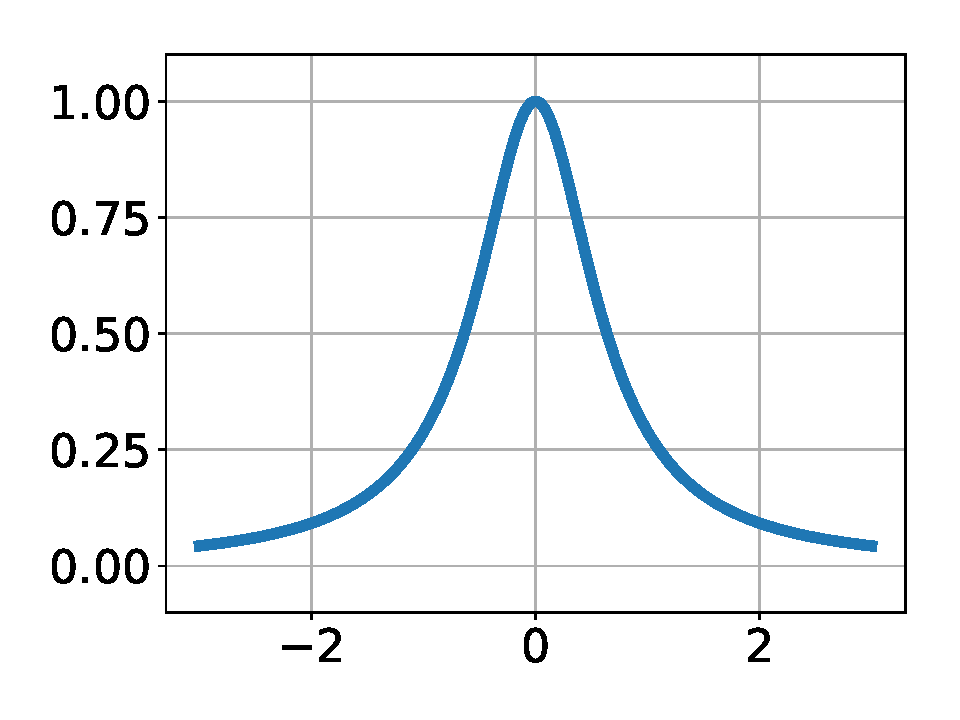
\includegraphics[width=0.4\textwidth]{images/motor_unit_assignment/phat.pdf}%
  \caption{Function $1/(1+a\,|x|^2)$, similar to $\hat{p}$ of \cref{eq:phat_kernel}, for $\sigma=1$.}%
  \label{fig:mu_phat}%
\end{figure}


If the kernel function $\hat{p}$ in \cref{eq:phat_kernel} is used to describe the probability of fiber $(i,j)$ to be in MU $k_\text{MU}$, then condition (iii) is fulfilled but conditions (i) and (ii) will not automatically be fulfilled. Instead of $\hat{p}$, a derived term $p(i,j,k_\text{MU})$ is introduced in the following that satisfies all requirements.

To ensure condition (ii), additional scalar factors $\lambda_k, k=1\dots n_\text{MU}$ for the MUs are introduced that yield the required exponential distribution.
To ensure condition (i), the term is normalized by a respective division. The resulting formulation is given as follows:
\begin{align}\label{eq:mu_p}
  p(i,j,k_\text{MU};\{\lambda_k\}_{1\dots n_\text{MU}}) = \dfrac{\hat{p}(i,j,k_\text{MU}) \cdot \lambda_{k_\text{MU}}}{\s{\ell_\text{MU}=1}{n_\text{MU}} \hat{p}(i,j,\ell_\text{MU}) \cdot \lambda_{\ell_\text{MU}}}.
\end{align}

Now, the factors $\{\lambda_k\}_{1\dots n_\text{MU}}$ have to be determined accordingly. Setting $\lambda_{k_\text{MU}} = q(k_\text{MU})$ would not yield the required exponential distribution of probabilities, because the MU center points $\bfx_{k_\text{MU}}$ have varying distances between each other.
Therefore, the accumulated total probability of all fibers to be associated to a particular MU is different for each MU. This is the case even before scaling with any factors $\{\lambda_k\}$.

Instead, the values of the factors have to be determined by solving a global optimization problem.
The objective function to be minimized is given by%
\begin{align}\label{eq:mus_objective}
  F(\{\lambda_k\}_{1\dots n_\text{MU}}) = \s{k_\text{MU}=1}{n_\text{MU}} \left(q(k_\text{MU}) - \s{i=1}{n}\s{j=1}{n}p(i,j,k_\text{MU};\{\lambda_k\}_{1\dots n_\text{MU}}) / n^2\right)^2.
\end{align}
It sums up the quadratic error for every MU between the desired, exponentially distributed probability $q(k_\text{MU})$ per fiber and the achieved probability per fiber under the current set of the scaling factors $\lambda_k$. 
The achieved probability is computed by a sum over all fibers $(i,j)$ and the formulated radial probability density function $p$ divided by $n^2$ to get the value per fiber.
After solving the optimization problem and plugging the factors $\{\lambda_k\}$ into \cref{eq:mu_p} we get every probability for a fiber to be in an MU by \cref{eq:mu_p}. The optimization problem is described in more detail in the following section.

\subsection{Algorithm to Solve the Optimization Problem}
The optimization problem to be solved in order to compute the scaling factors in \cref{eq:mu_p} can be stated as:
\begin{align}\label{eq:mus_opt}
  \text{``Find}\quad \{\lambda_k\}_{1\dots n_\text{MU}} \text{ with } \lambda_k > 0 \quad \text{ s.t. } \quad F(\{\lambda_k\}_{1\dots n_\text{MU}}) \quad \text{ is minimal''.}
\end{align}
The objective function $F$ was given in \cref{eq:mus_objective}. The solution is obtained by a Quasi-Newton method, more specifically the limited-memory version of the \emph{Broyden}-\emph{Fletcher}-\emph{Goldfarb}-\emph{Shanno} algorithm with box constraints by the authors of \cite{byrd1995limited}. Their Fortran implementation is made accessible in Python by the \emph{SciPy Optimize} package.

With increasing number $n^2$ of fibers and increasing number $n_\text{MU}$ of MUs, the evaluation duration for the objective function and the number of optimization parameters increases. For numbers about $n^2 > 1000$ and $n_\text{MU} > 25$, the solution times become unfeasible.

As a remedy we develop an algorithm to split the large optimization problem into multiple smaller ones which reduces the total runtime. 
The set of factors $\{\lambda_k\}_{1\dots n_\text{MU}}$ is partitioned into chunks, i.e., subsets of given size $n_\text{per\_chunk}$ leading to a total of $n_\text{chunks} = \lceil n_\text{MU} / n_\text{per\_chunk} \rceil$ chunks.
Remainder chunks towards the end potentially get one set element less. 
The factors for chunk number $c$ are selected in a strided manner as $\{\lambda_k\}$ with indices ${k=c, c+n_\text{chunks}, c+2\,n_\text{chunks}, \dots}$. For example, for $n_\text{MU}=13$ and $n_\text{per\_chunk}=4$ we get chunks of sizes $4,3,3,3$ and subsequently solve for $\{\lambda_k\}$ with $k \in \{1,5,9,13\}$, $\{2,6,10\}$, $\{3,7,11\}$, $\{4,8,12\}$.

A number of $n_\text{chunks}$ optimization problems is solved subsequently where the optimization parameters are each time given by the next chunk. During this loop, more and more scalar factors are determined.
Initially, all scalar factors $\lambda_k$ are set to one. 
After each solved optimization problem, the respective $\lambda_k$ values are updated with the values of the found minimizer.
The number $n_\text{factors\_up\_to\_chunk}$ of already solved scalar factors up to the current iteration starts with zero and increases by $n_\text{per\_chunk}$ after each iteration, finally arriving at $n_\text{MU}$ after the last iteration.

These smaller optimization problems have a similar formulation as the overall problem with different values for some variables.
The formulation of the optimization problem involves \cref{eq:mus_q,eq:phat_kernel,eq:mu_p,eq:mus_objective}. 
The number $n_\text{MU}$ of motor units in \cref{eq:mu_p,eq:mus_objective} is replaced by the number $(n_\text{factors\_up\_to\_chunk}+n_\text{per\_chunk})$ of factors that will have been solved after the current iteration. 
%This means that only so many MUs are considered at this iteration of the algorithm.

As each of the small optimization schemes only solves for $n_\text{per\_chunk}$ factors, the argument of the objective in \cref{eq:mus_objective} contains only the factors of the current chunk.
The other $n_\text{factors\_up\_to\_chunk}$ factors in the definition that are not given by the argument of the objective are set to the solutions obtained in previous iterations.

The indexing of the MU center positions $\bfx_{k_\text{MU}}$ in \cref{eq:phat_kernel} is adjusted such that only the MUs up to and including the current chunk are considered. The indexing in the exponential progression formulated by \cref{eq:mus_q}, however, stays the same, here the argument $k_\text{MU}$ of the function $q$ refers to the full set of MUs.

In summary, the iteratively considered settings contain an increasing number of MUs. The number of optimization parameters and, thus, new MUs is kept constant while the number of summands in the objective function increases. In consequence, the evaluation of the objective function gets more expensive with increasing iteration number while the size of the optimization problem stays constant. The latter has more influence on the optimizer duration.
By increasing the chunk size $n_\text{per\_chunk}$, the size of the small optimization problems can be decreased to any value. This makes the presented algorithm applicable for any large number $n_\text{MU}$ of MUs.

The result in this approach is not exactly the same as if one big optimization problem including all scalar factors at once would be solved. However, the error is small because of the interleaved MUs indices that are considered in every iteration. Because the resulting MU distribution finally gets drawn from the computed random probability distribution the error is hardly noticable in the result.

\subsection{Sampling Motor Unit Indices from the Given Probabilities}

The next step is to assign actual MU numbers to every fiber. Drawing samples $Y$ with the given probabilities $p(i,j,k_\text{MU})$ is done using inverse transform sampling. The inverse cumulative distribution function (CDF) $F_p^{-1}(k_\text{MU})$ is applied onto a random value $X$ drawn from a continuous uniform distribution $\mathcal{U}$:
\begin{align*}
  Y = F_p^{-1}(X)\quad \text{with }X\sim \mathcal{U}\big(0,F_p(n_\text{MU})\big), \quad F_p(k_\text{MU}) = \s{\ell_\text{MU}=1}{k_\text{MU}} p(i,j,\ell_\text{MU}).
\end{align*}
Computing the inverse of the CDF is computationally cheap as the probabilities are discrete and, thus, a loop over the values of the CDF suffices.

To reduce outliers during the random sampling where some MUs get exceptionally little fibers (such as none) or exceptionally many fibers assigned, the sampling procedure is performed five times.
Each time, a histogram with bins for the MUs is computed and provides the number of fibers per MUs. For all MUs $k$ that have zero fibers assigned, the one fiber where the probability for the respective MU $k$ is highest is determined. This is usually the fiber closest to the center point $\bfx_k$ of the MU $k$. The MU assignment of this fiber is changed to $k$, such that the MU $k$ is no longer empty but is associated to one fiber.

In each of the five iterations, the squared error between the sampled MU sizes and the expected sizes according to the probabilities, given by $q(k_\text{MU})\cdot n^2$ is computed. The MU assignment of the iteration that yielded the smallest error is used for the final result of method 1.


\section{Method 2: Assignment of Motor Units to a Selection of Fibers}\label{sec:method2_selection}

The second method proceeds similar to the first method in that at first the probability for a specific MU is defined for any fiber $(i,j)$ in the $n \times n$ grid. Then the actual MU assignments are sampled from the probability distributions. The difference to the first method is that any fiber is also allowed to not be assigned to any MU. This makes the definition of the probabilities easier and no optimization is required.

The three conditions defined in \cref{sec:stochastic_formulation_and_algorithm} are also imposed for the second method. The definition of the MU center positions $\bfx_{k_{MU}}$ follows the same low-discrepancy series. Also, the radial kernel function \cref{eq:phat_kernel} can be reused to describe the spatial distribution of probability for a given MU. Instead of \cref{eq:mu_p}, the probability is formulated directly as the product of the kernel function $\hat{p}$ and the exponential progression $q$:
\begin{align*}
  \tilde{p}(i,j,k_\text{MU}) = \hat{p}(i,j,k_\text{MU}) \cdot q(k_\text{MU}).
\end{align*}
%
To ensure that the function is within the bounds of a probability, $p \leq 1$, the result is divided by the maximum occuring value,%
\begin{align*}
  p(i,j,k_\text{MU}) = \dfrac{\tilde{p}(i,j,k_\text{MU})}{\max\limits_{\substack{\bar{i},\bar{j} = 1,\dots,n\\\bar{k}_\text{MU}=1,\dots,n_\text{MU}}} \tilde{p}(\bar{i},\bar{j},\bar{k}_\text{MU})}.
\end{align*}
%

In the sampling step, for every fiber $(i,j)$ the probabilities $p(i,j,k_\text{MU}), k_\text{MU}=1,\dots,n_\text{MU}$ for the MUs and the remaining probability $\bar{p} = 1-\sum_{k_\text{MU}} p(i,j,k_\text{MU})$ are computed. Then, the MU index is randomly drawn from the set of numbers $\{1,\dots,n_\text{MU}\}$ and a \say{null} event that corresponds to no assigned MU, according to the computed probabilities $p$ and $\bar{p}$. 

As a result, we get MUs that satisfy all three conditions formulated in \cref{sec:stochastic_formulation_and_algorithm}, including the approximate exponential progression of the MU sizes. However, the resulting number of fibers with assigned MU is an outcome of the algorithm and cannot be prescribed.

\section{Assignment of Different Motor Units for Neighboring Fibers}\label{sec:method3_modification}

As mentioned in \cref{sec:mu_intro}, one observation in staining experiments was that the fibers of an MU typically do not touch each other, i.e., neighboring fibers always belong to different MUs.
However, the presented methods 1 and 2 assign neighboring fibers with a high probability to the same MU. To create a grid with an MU assignment that avoids this behavior, the idea is to interleave four smaller grids where the MU assignments were obtained independently of each other but with the same parameters. In the following, this method is named \say{method 1a} and \say{2a} depending on whether the partial grids were handled with method 1 or 2.

First, either method 1 or method 2 are applied four times to smaller grids of fibers, the \emph{partial grids}, as visualized in \cref{fig:interleaving_scheme}. The partial grids contain $n_\text{part} \times n_\text{part} = n/2 \times n/2$ fibers. In each partial grid, MU assignments with $n_\text{MU,part} = n_\text{MU}/4$ MUs are created. The basis $b$ is changed to $b_\text{part} = b^4$ and the standard deviation of the kernel function is changed to $\sigma_\text{part} = \sigma/2$. In result, we get the same exponential distribution of number of fibers per MU on every partial grid.

The four smaller grids are then merged according to the scheme shown in \cref{fig:interleaving_scheme}. Fibers of the first partial grid directly touch only fibers of the third and fourth grids and touch fibers of the second partial grid diagonally. By using this scheme, neighboring fibers in any of the partial grids are always separated by fibers of other grids. 

The MU indices that are assigned in the partial grids are mapped to the resulting, large grid also in an interleaved manner. MU $k$ of the $l$\emph{th} grid is mapped to the resulting MU $(4\,(k-1)+\ell)$. For illustration, the MUs 1,2,3 of the first grid are mapped to MUs $1,5,9$, MUs 1,2,3 of the second grid are mapped to MUs $2,6,10$, etc. Since the MU sizes in the partial grids follow the defined exponential progression, this also holds for the final MUs. 

The location of the MU center points is determined by contiguous elements of the same Weyl sequence given in \cref{eq:weyl} for all partial grids. First, all MU center points for the first partial grid are assigned, then for the second, third and forth. By this construction, all MU center points are distributed with similar spacing between each other and the placement of similar sized MUs close to each other is avoided.

\begin{figure}%
  \centering%
  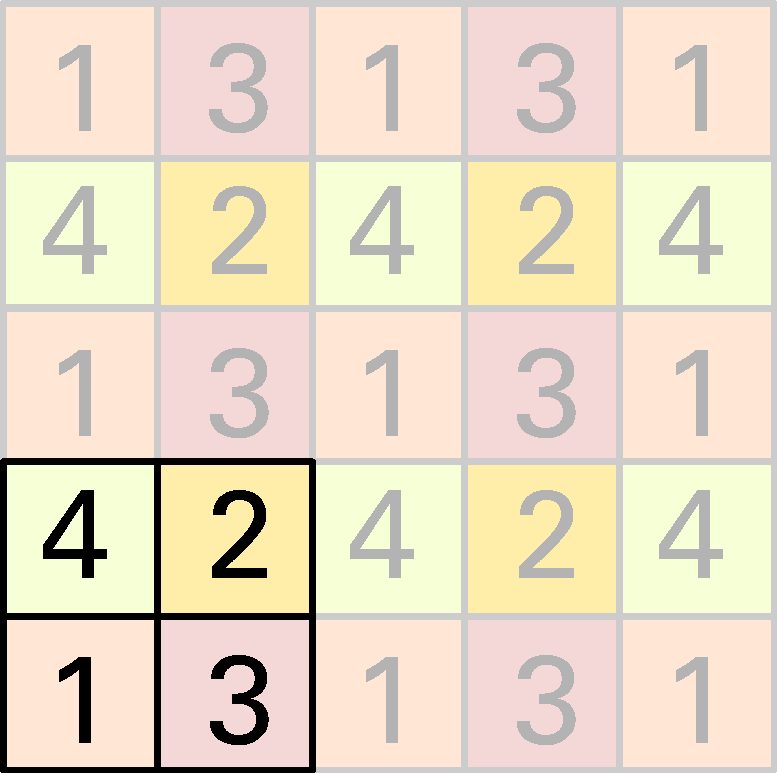
\includegraphics[width=0.4\textwidth]{images/motor_unit_assignment/interleaving_scheme.pdf}%
  \caption{Repeating scheme for interleaving the four partial grids. The partial grids are indicated by the numbers and have different colors. The pattern is highlighted at the bottom left of the figure.}%
  \label{fig:interleaving_scheme}%
\end{figure}

\section{Results and Discussion}\label{sec:mu_results_and_discussion}

In the following, results of the methods described in \cref{sec:method1_assignment,sec:method2_selection,sec:method3_modification} with different parameters are presented.
\Cref{fig:mus_results1} shows the resulting assignment of MUs to fibers for methods 1 and 2. The number of fibers per coordinate direction is $n=13$, a number of $n_\text{MU} = 10$ MUs is considered and two different values for the kernel function parameter $\sigma$ are used.

In \cref{fig:MU_fibre_distribution_13x13_10_2d_fiber_distribution}, method 1 is used with basis $b=1.2$ and a kernel function with standard deviation of a tenth of the grid, $\sigma=n/10$. Each square represents one fiber, their colors refer to the MU index as indicated by the legend. Colored crosses visualize the center points $\bfx_{k_\text{MU}}$ of the respective MUs.

It can be seen that the MU territories, i.e., the regions of the fibers of an MU are located around the center points of the MUs. Because of the random sampling, the fibers of an MU are not all located closely together but spread over a larger area. Especially for MU 8, depicted by light orange color, some fibers are located further away from the center point, which is approximately at the center of the grid. On the other hand, for MU 10 most of the red marked fibers are located close to the center point of the MU, which can be found in the center of the lower third of the grid.

\begin{figure}%
  \centering%
  \begin{subfigure}[t]{0.48\textwidth}%
    \centering%
    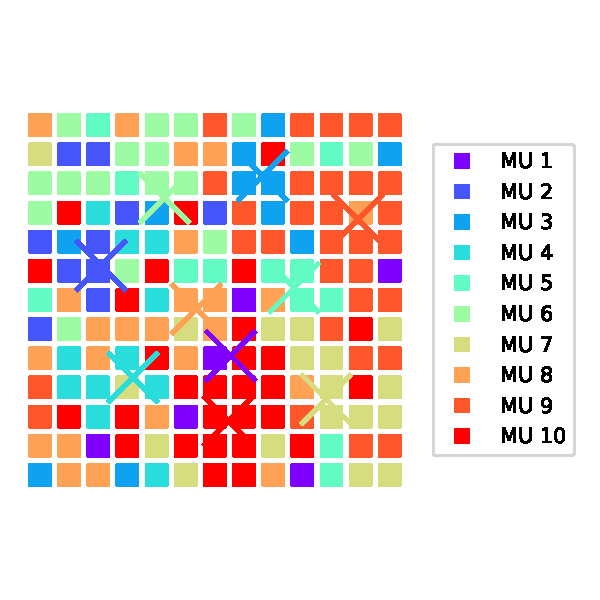
\includegraphics[width=\textwidth]{images/motor_unit_assignment/MU_fibre_distribution_13x13_10_2d_fiber_distribution.pdf}%
    \caption{Result for method 1 with $\sigma = n/10 = 1.3$}%
    \label{fig:MU_fibre_distribution_13x13_10_2d_fiber_distribution}%
  \end{subfigure}
  \quad
  \begin{subfigure}[t]{0.48\textwidth}%
    \centering%
    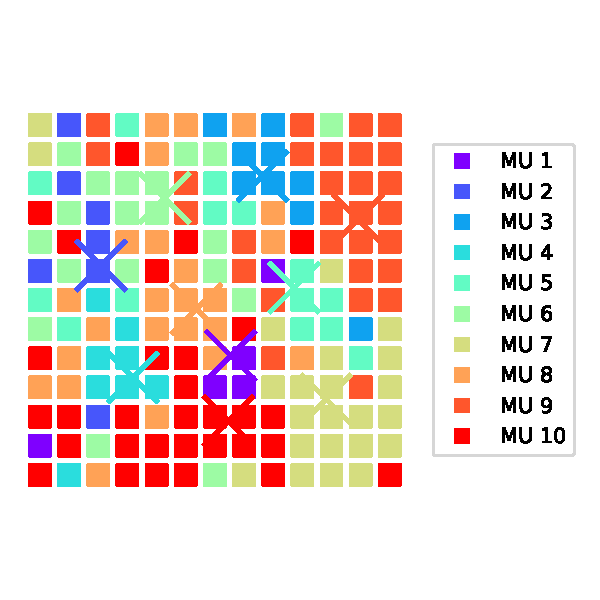
\includegraphics[width=\textwidth]{images/motor_unit_assignment/MU_fibre_distribution_13x13_10_2d_fiber_distribution_sigma.pdf}%
    \caption{Result for method 1 with $\sigma = n/100 = 0.13$}%
    \label{fig:MU_fibre_distribution_13x13_10_2d_fiber_distribution_sigma}%
  \end{subfigure}
  \begin{subfigure}[t]{0.48\textwidth}%
    \centering%
    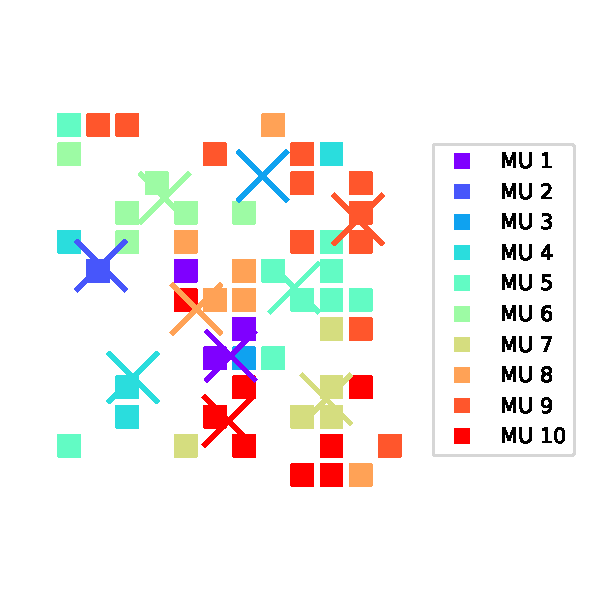
\includegraphics[width=\textwidth]{images/motor_unit_assignment/MU_fibre_distribution_sparse_13x13_10_2d_fiber_distribution.pdf}%
    \caption{Result for method 2 with $\sigma = n/10 = 1.3$, only 54 out of 169 fibers, i.e., \SI{32}{\percent} have an assigned motor unit.}%
    \label{fig:MU_fibre_distribution_sparse_13x13_10_2d_fiber_distribution}%
  \end{subfigure}
  \quad
  \begin{subfigure}[t]{0.48\textwidth}%
    \centering%
    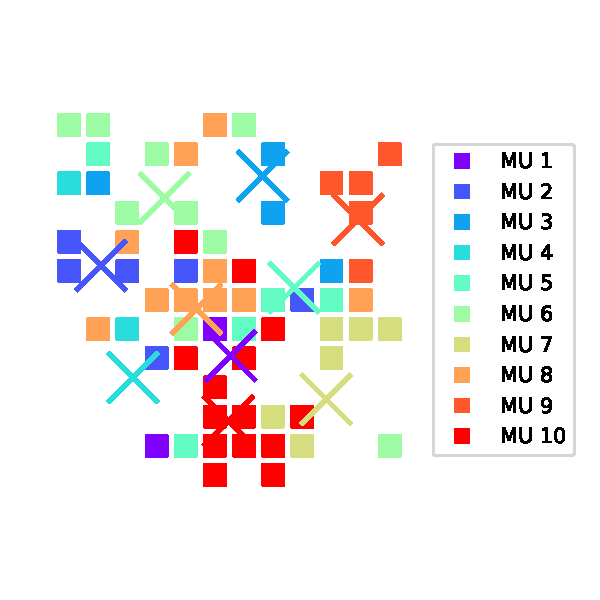
\includegraphics[width=\textwidth]{images/motor_unit_assignment/MU_fibre_distribution_sparse_13x13_10_sigma_2d_fiber_distribution.pdf}%
    \caption{Result for method 2 with $\sigma = n/100 = 0.13$, only 63 out of 169 fibers, i.e., \SI{37}{\percent} have an assigned motor unit.}%
    \label{fig:MU_fibre_distribution_sparse_13x13_10_sigma_2d_fiber_distribution}%
  \end{subfigure}
  \caption{Resulting MU assignments to a grid of $n\times n = 13 \times 13 = 169$ fibers. Each MU is represented by a color, the MU center points $\bfx_{k_\text{MU}}$ are the same for all scenarios and are shown by the colored crosses.}%
  \label{fig:mus_results1}%
\end{figure}%

The histogram for the setting considered in \cref{fig:MU_fibre_distribution_13x13_10_2d_fiber_distribution} is shown in \cref{fig:MU_fibre_distribution_13x13_10_fiber_distribution}. It can be seen that the number of fibers per motor unit approximately follows the prescribed exponential function with basis $b=1.2$. The observed deviation is due to the random sampling.

\begin{figure}%
  \centering%
  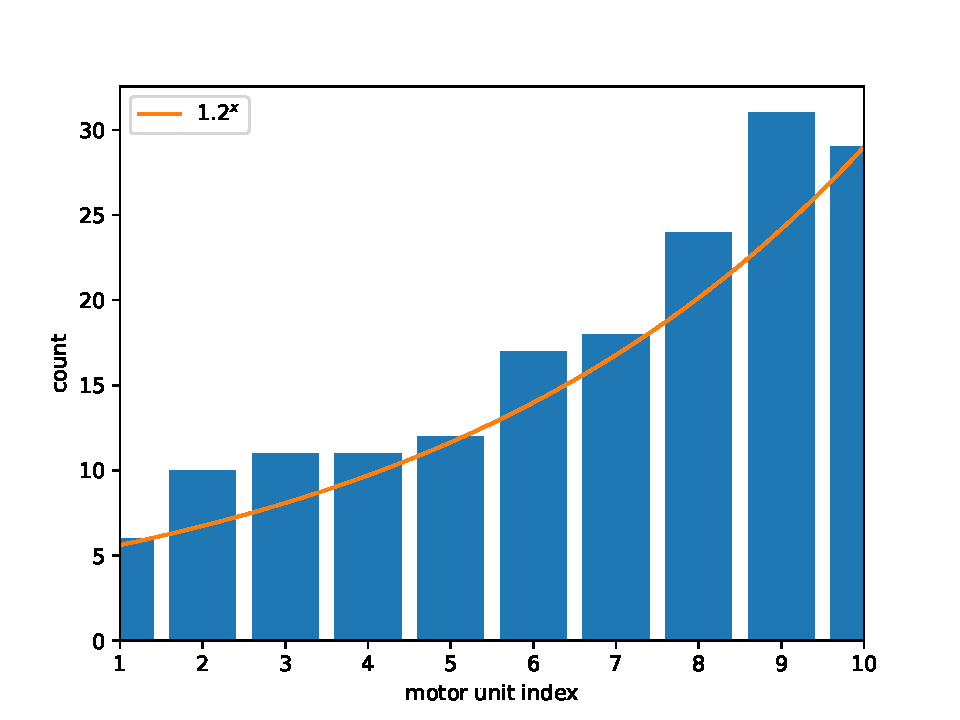
\includegraphics[width=0.8\textwidth]{images/motor_unit_assignment/MU_fibre_distribution_13x13_10_fiber_distribution.pdf}%
  \caption{Histogram of the number of fibers per MU in \cref{fig:MU_fibre_distribution_13x13_10_2d_fiber_distribution}. The orange line corresponds to the ideal exponential distribution $y=c\cdot 1.2^x$.}%
  \label{fig:MU_fibre_distribution_13x13_10_fiber_distribution}%
\end{figure}

\Cref{fig:mu_kernel_fkt} shows the values of the probability function of a specific MU for all fibers, formulated in \cref{eq:mu_p}. \Cref{fig:MU_fibre_distribution_13x13_10_fibers_mu3,fig:MU_fibre_distribution_13x13_10_fibers_mu9} correspond to the scenario considered in \cref{fig:MU_fibre_distribution_13x13_10_2d_fiber_distribution}. The comparison shows that the probability is highest around the center of MU 3 and MU 9, respectively. When moving away from the MU centers, the probability follows approximately the shape of the radial kernel function in \cref{eq:phat_kernel}.
An image of the radial kernel function in higher resolution is given by \cref{fig:MU_fibre_distribution_37x37_50_fibers_mu41}, where the probability function is depicted for MU 41 in a scenario with 50 MUs in a grid of $37 \times 37$ fibers.

It can be observed, however, that the probability distribution in \cref{fig:MU_fibre_distribution_13x13_10_fibers_mu3,fig:MU_fibre_distribution_13x13_10_fibers_mu9} does not entirely follow the kernel function. The effects of the scaling factors $\{\lambda_k\}$ in \cref{eq:mu_p} are visible, e.g., at the top-most and right-most fibers. There, the probability increases again compared to the interior of the grid. The purpose of the scaling factors is to enforce the exponential distribution of MU sizes.

\begin{figure}%
  \centering%
  \begin{subfigure}[t]{0.31\textwidth}%
    \centering%
    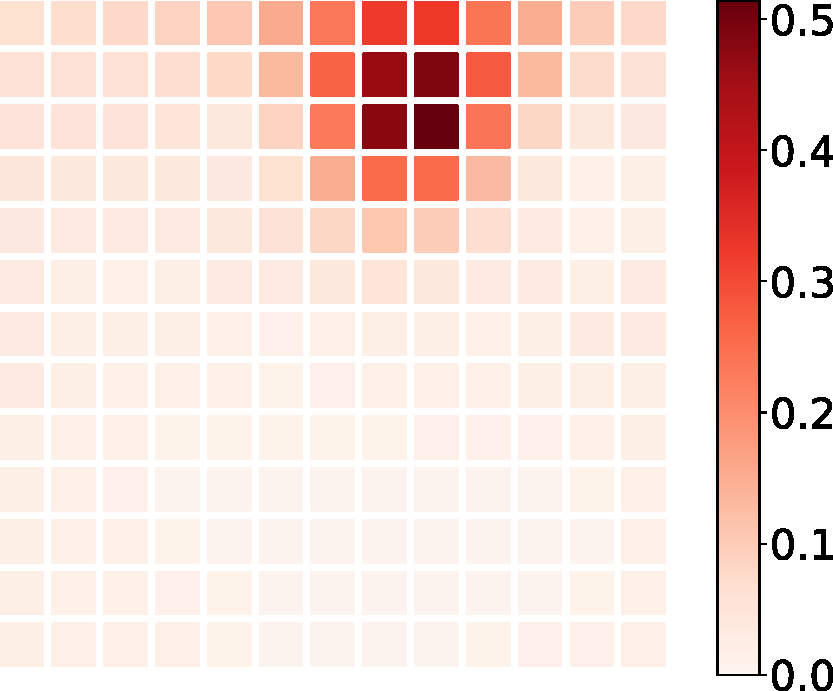
\includegraphics[width=\textwidth]{images/motor_unit_assignment/MU_fibre_distribution_13x13_10_fibers_mu3.pdf}%
    \caption{$n=13, \sigma = n/10 = 0.13$, MU 3}%
    \label{fig:MU_fibre_distribution_13x13_10_fibers_mu3}%
  \end{subfigure}
  \quad
  \begin{subfigure}[t]{0.31\textwidth}%
    \centering%
    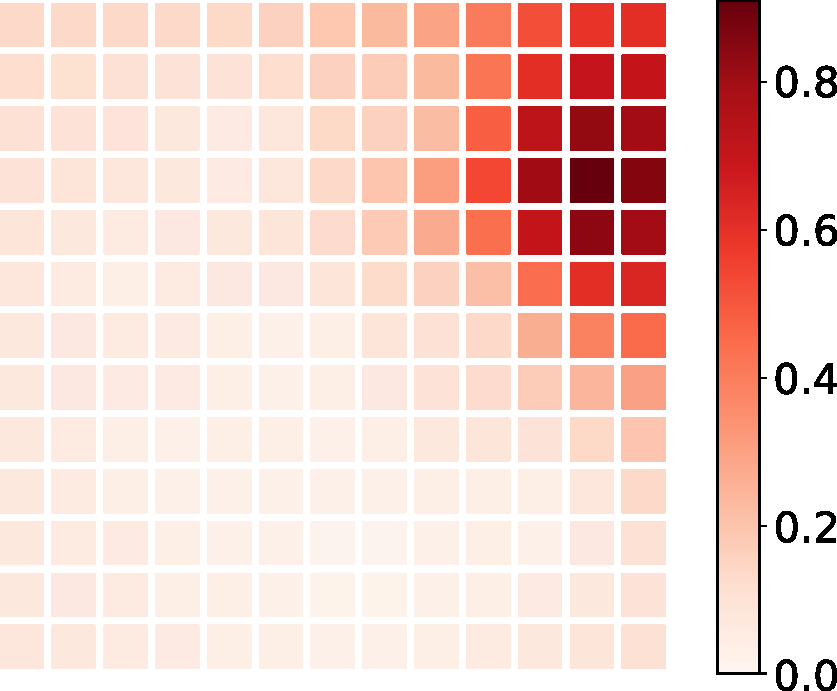
\includegraphics[width=\textwidth]{images/motor_unit_assignment/MU_fibre_distribution_13x13_10_fibers_mu9.pdf}%
    \caption{$n=13, \sigma = n/10 = 0.13$, MU 9}%
    \label{fig:MU_fibre_distribution_13x13_10_fibers_mu9}%
  \end{subfigure}
  \quad
  \begin{subfigure}[t]{0.31\textwidth}%
    \centering%
    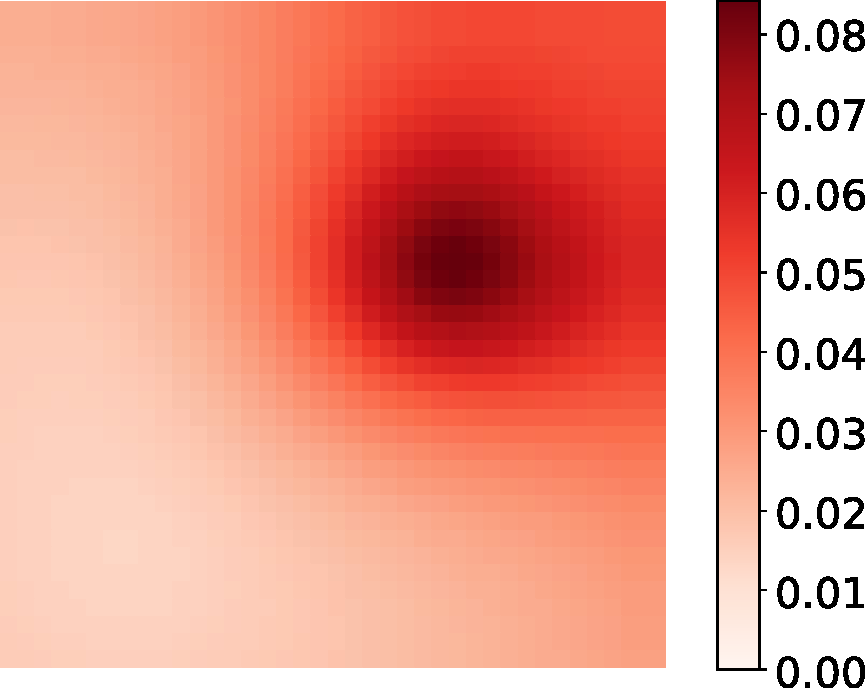
\includegraphics[width=\textwidth]{images/motor_unit_assignment/MU_fibre_distribution_37x37_50_fibers_mu41.pdf}%
    \caption{$n=37, \sigma = n/10 = 0.37$, MU 41}%
    \label{fig:MU_fibre_distribution_37x37_50_fibers_mu41}%
  \end{subfigure}
  \caption{Probability at every fiber to be in a given MU, for different grid sizes and number of MUs.}%
  \label{fig:mu_kernel_fkt}%
\end{figure}%

This effect is illustrated more clearly in \cref{fig:MU_fibre_distribution_13x13_10_pdf}. It shows the value of $p(i,j,k_\text{MU})$ for the top right fiber in the grid, $(i,j)=(13,13)$, for all values of $k_\text{MU}$. The blue curve indicates the probability that results from the kernel functions, only according to the distance of the top right fiber to the respective MU centers. In other words, the scaling factors $\{\lambda_k\}_{1\dots n_\text{MU}}$ are removed or equivalently set to one. By inspecting again \cref{fig:MU_fibre_distribution_13x13_10_2d_fiber_distribution}, it can be seen that the MU centers of MUs 9, 3 and 5 are---in this order---closest to the top right fiber whereas MU 4 and 10 are the furthest away. Consequently, the blue curve in \cref{fig:MU_fibre_distribution_13x13_10_pdf} has peaks at 9, 3 and 5 and low values for 4 and 10.

When incorporating the scaling factors $\{\lambda_k\}_{1\dots n_\text{MU}}$ that were found by the optimization problem in \cref{eq:mus_opt}, the probabilities change to the orange curve. It can be seen that the probability for the fiber to be in MU 9 increases. MU 9 which is expected to have a rather high number of fibers according to the exponential progression.
It gets more fibers from the top right corner. The areas left to and below the center of MU 9 are at the same time close to the centers of MU 3 and 5 and therefore can also be occupied by fibers of MUs 3 and 5. Thus, the optimization performs an exchange where MU 9 forgoes the bottom and left fibers and, conversely, obtains portions of the fibers in the top right area from MUs 3 and 5. Consequently, the probability in \cref{fig:MU_fibre_distribution_13x13_10_pdf} decreases for MUs 3 and 5. The shape of the final probability distribution for MU 9 in \cref{fig:MU_fibre_distribution_13x13_10_fibers_mu9} is the kernel function stretched to the top and right.
By looking at \cref{fig:MU_fibre_distribution_13x13_10_2d_fiber_distribution}, it can be seen that, by chance, the top right fiber indeed gets assigned to MU 9.

\begin{figure}%
  \centering%
  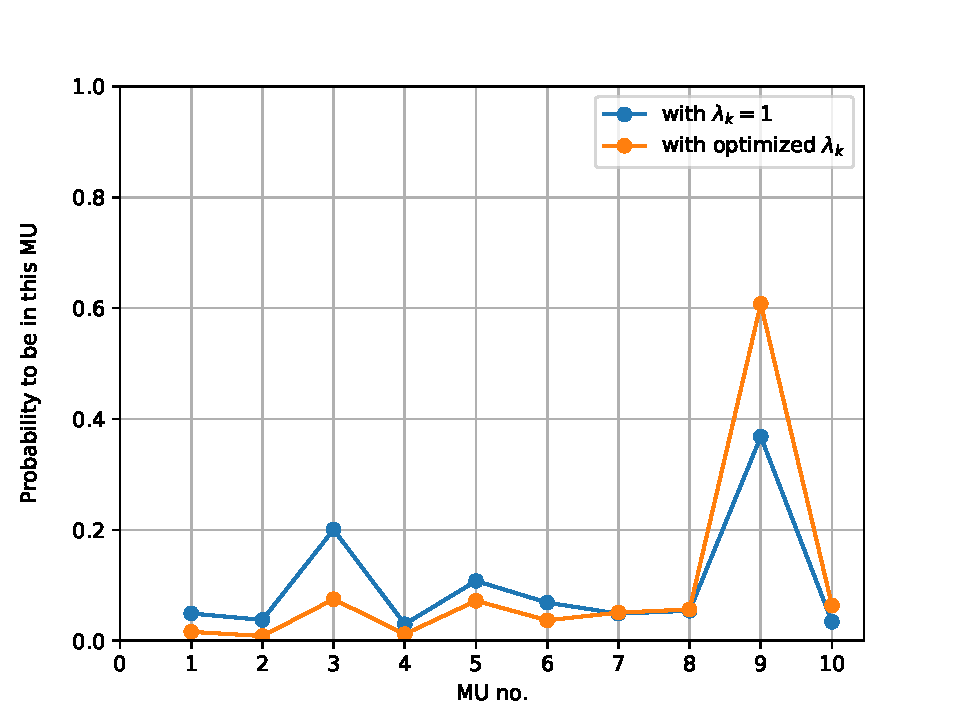
\includegraphics[width=0.8\textwidth]{images/motor_unit_assignment/MU_fibre_distribution_13x13_10_pdf.pdf}%
  \caption{Probability of the top right fiber in the $13 \times 13$ grid to be in a given MU, without considering the scaling factors $\{\lambda_k\}_{1\dots n_\text{MU}}$ (blue) and including the scaling factors (orange).}%
  \label{fig:MU_fibre_distribution_13x13_10_pdf}%
\end{figure}

The influence of the kernel width $\sigma$ is demonstrated by comparing \cref{fig:MU_fibre_distribution_13x13_10_2d_fiber_distribution} with \cref{fig:MU_fibre_distribution_13x13_10_2d_fiber_distribution_sigma}. In \cref{fig:MU_fibre_distribution_13x13_10_2d_fiber_distribution_sigma} the value of $\sigma$ is only a tenth of the value in \cref{fig:MU_fibre_distribution_13x13_10_2d_fiber_distribution}. All other parameters are the same such that a similar exponential distribution of MU sizes is obtained. It can be seen that the MU territories are less interleaved and have clearer borders. For example, the territory of MU 7 at the bottom left of the domain has a cohesive shape in \cref{fig:MU_fibre_distribution_13x13_10_2d_fiber_distribution_sigma} whereas the respective fibers are more scattered in \cref{fig:MU_fibre_distribution_13x13_10_2d_fiber_distribution}.

In comparison, the results for method 2 with the same two values of $\sigma$ are shown in \cref{fig:MU_fibre_distribution_sparse_13x13_10_2d_fiber_distribution,fig:MU_fibre_distribution_sparse_13x13_10_sigma_2d_fiber_distribution}. All other parameters are kept the same. It can be seen how method 2 only associates some fibers with MUs. For the larger standard deviation $\sigma$ in \cref{fig:MU_fibre_distribution_sparse_13x13_10_2d_fiber_distribution}, only \SI{32}{\percent} of the fibers get assigned to a MU, for the smaller value of $\sigma$, the fraction is slightly higher with \SI{37}{\percent}. Similar to method 1, the effect of more cohesive MU territories for smaller $\sigma$ values can also be observed in the results of method 2.

Next, the two methods 1 and 2 are investigated for a higher number of $n_\text{MU}=100$ motor units and a grid of $n \times n=67 \times 67 = \num{4489}$ fibers.

\Cref{fig:MU_fibre_distribution_67x67_100_mu_positions} shows the MU center points $\bfx_{k_\text{MU}}$. The color corresponds to the MU index and follows the same rainbow color scheme as in \cref{fig:mus_results1}. Since the construction scheme is the deterministic Weyl sequence in \cref{eq:weyl}, the first 10 MU center positions are the same as for the scenario with $n_\text{MU}=10$. It can be seen that the MU centers have similar distances throughout the grid and that, in general, MUs located next to each other have different colors and therefore are differently sized.

\Cref{fig:MU_fibre_distribution_67x67_100_fiber_distribution} shows the histogram of the MUs, i.e., the number of fibers per MU. Following \cite{Enoka2001} the prescribed basis for the exponential progression was reduced because of the higher number of fibers. It was set to $b=1.05$. It can be seen that the resulting MU size distribution closely matches the prescribed function. Because the ratio of fibers to MUs (4489/100) is higher than in the previous setting (169/10) the deviation of the realized MU sizes from the prescribed curve appears smaller than in \cref{fig:MU_fibre_distribution_13x13_10_fiber_distribution}.

\Cref{fig:MU_fibre_distribution_67x67_100_some_2d_fiber_distribution.pdf} shows the result for method 1. The width of the radial kernel function was chosen as $\sigma = n/100 = \num{0.67}$. Only the fibers of five selected MUs and their center points are visualized for better clearity.

The algorithm for the 4489 fibers and 100 MUs was performed with a  chunk size of $n_\text{per\_chunk}=10$, yielding a total number of $n_\text{chunks}=10$ chunks. The runtime was \SI{45}{\min} \SI{53.5}{\sec} on a single core of an Intel Core i5-6300U CPU with base frequency of 2.40GHz and 19.5 GiB of RAM.

\Cref{fig:MU_fibre_distribution_sparse2_67x67_100_2d_fiber_distribution} shows the result for method 2. All resulting fibers that were associated to an MU are shown as gray or colored squares, leaving white spaces for unassigned fibers. Again, only the fibers of five selected MUs are colored. The kernel parameter was set to $\sigma = 0.04\cdot n = \num{2.68}$ which resulted in 2328 of 4489 fibers or \SI{52}{\percent} of the fibers being assigned an MU. When the parameter is instead set to $\sigma = n/100  = \num{0.67}$ as in the study with 10 MUs before, the result assigns only 136 fibers or \SI{3}{\percent}. This shows that method 2 is very sensitive to the choice of the standard deviation parameter $\sigma$.

The comparison with \cref{fig:MU_fibre_distribution_67x67_100_some_2d_fiber_distribution.pdf} shows that the resulting MU territories are more dispersed than for method 1. This can be explained with the higher value of $\sigma$. Obtaining \say{sharper} MU territories would require a smaller $\sigma$, however, this results in less fibers being assigned to MUs.

Furthermore, \cref{fig:MU_fibre_distribution_sparse2_67x67_100_2d_fiber_distribution} shows that the fiber density decreases towards the outer border of the domain. In reality, staining studies on skeletal muscles do not find this effect.
%In an electrophysiology simulation with muscle fibers where the aim is to compute EMG signals on the surface of a muscle, this effect is not desired, as the border of the domain is the important part that contributes to the measurements of surface EMG.

An advantage of method 2 over method 1 is that we do not have to solve any optimization problem. In consequence, the algorithm for the scenario in \Cref{fig:MU_fibre_distribution_sparse2_67x67_100_2d_fiber_distribution} was completed in \SI{8}{\sec} on the same hardware as before.

\begin{figure}%
  \centering%
  \begin{subfigure}[t]{0.48\textwidth}%
    \centering%
    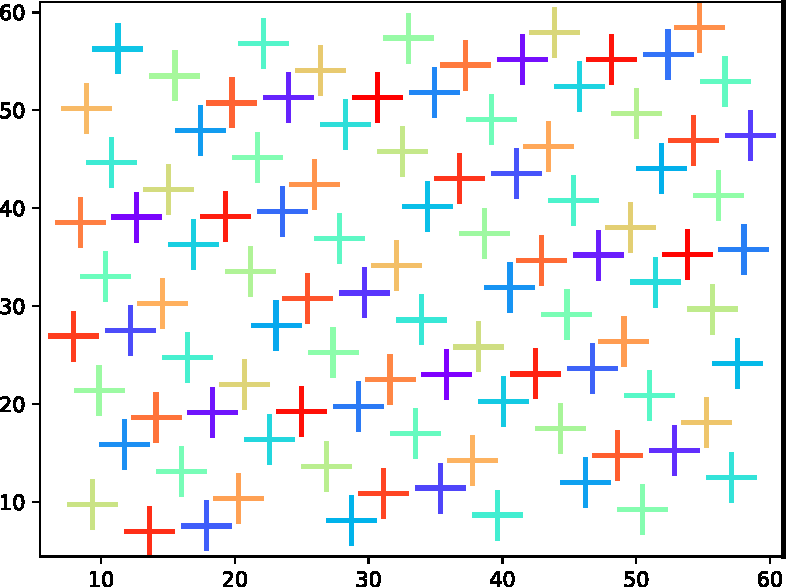
\includegraphics[width=\textwidth]{images/motor_unit_assignment/MU_fibre_distribution_67x67_100_mu_positions.pdf}%
    \caption{MU center points.}%
    \label{fig:MU_fibre_distribution_67x67_100_mu_positions}%
  \end{subfigure}
  \quad
  \begin{subfigure}[t]{0.48\textwidth}%
    \centering%
    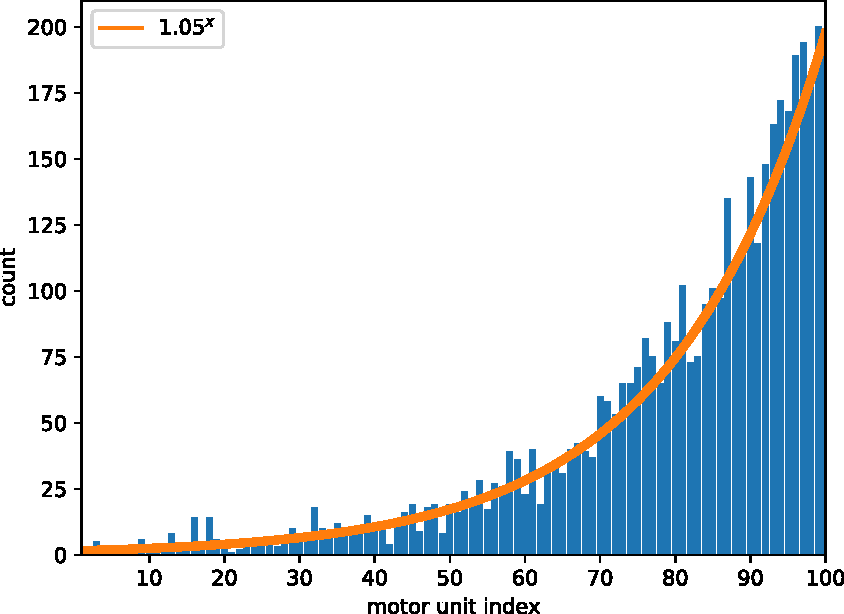
\includegraphics[width=\textwidth]{images/motor_unit_assignment/MU_fibre_distribution_67x67_100_fiber_distribution.pdf}%
    \caption{Histogram of number of fibers assigned to MUs (blue) and the prescribed exponential progression $y=c\cdot 1.05^x$ (orange).}%
    \label{fig:MU_fibre_distribution_67x67_100_fiber_distribution}%
    %total number of fibers: 4489
  %  MU 11, n. fibers optimal: 2.802, n. fibers expected: 0.945, realized: 1
  %MU 41, n. fibers optimal: 12.108, n. fibers expected: 8.809, realized: 15
  %MU 61, n. fibers optimal: 32.126, n. fibers expected: 30.439, realized: 29
  % MU 81, n. fibers optimal: 85.241, n. fibers expected: 127.908, realized: 118
  %MU 91, n. fibers optimal: 138.849, n. fibers expected: 137.036, realized: 123
  
  \end{subfigure}
  \begin{subfigure}[t]{0.48\textwidth}%
    \centering%
    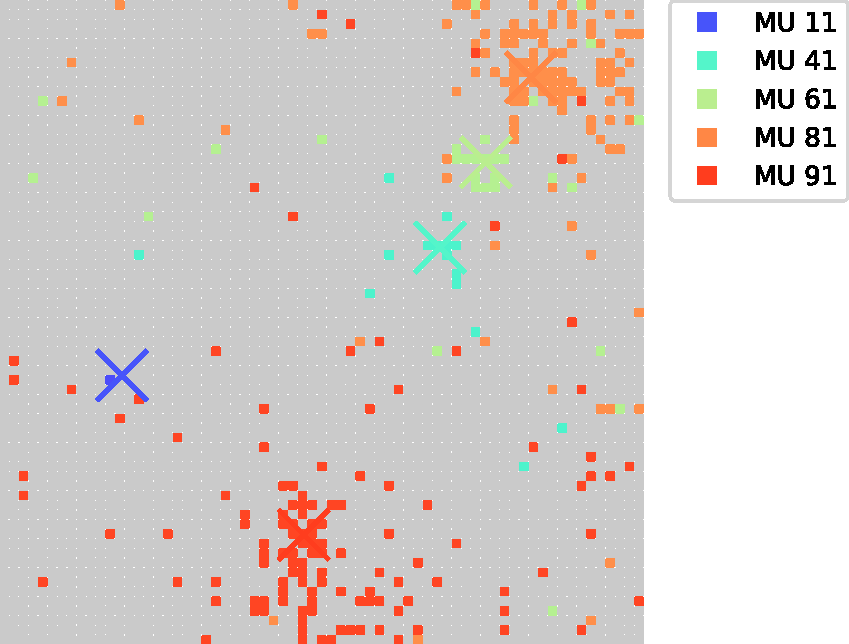
\includegraphics[width=\textwidth]{images/motor_unit_assignment/MU_fibre_distribution_67x67_100_some_2d_fiber_distribution.pdf}%
    \caption{Result of method 1 with $\sigma = n/100 = \num{0.67}$. The colored fibers are assigned to one of five selected MUs: 11, 41, 61, 81 and 91. The MU sizes are: 
    MU 11: 1 fiber,
    MU 41: 2 fibers,
    MU 61: 15 fibers,
    MU 81: 32 fibers,
    MU 91: 72 fibers}%
    \label{fig:MU_fibre_distribution_67x67_100_some_2d_fiber_distribution.pdf}%
  \end{subfigure}
  \quad
  \begin{subfigure}[t]{0.48\textwidth}%
    \centering%
    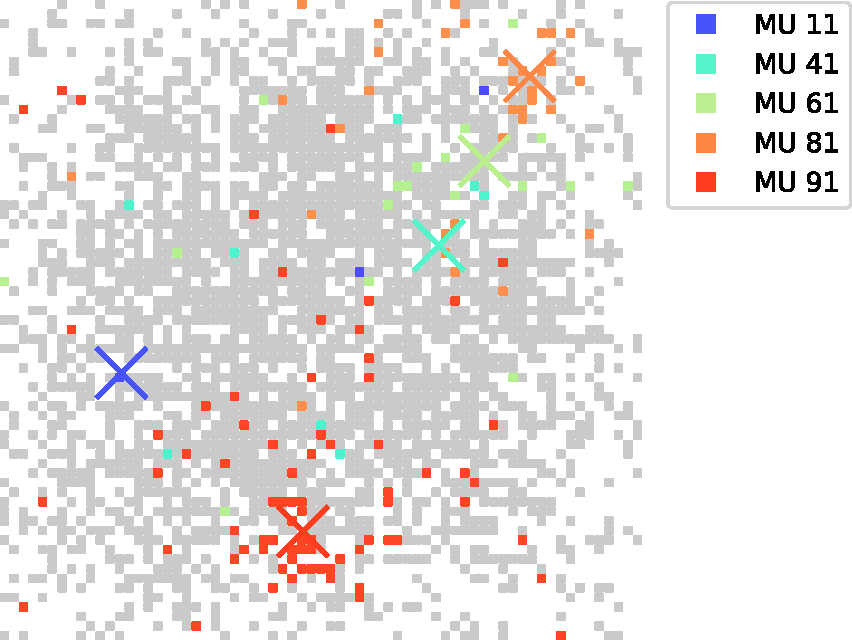
\includegraphics[width=\textwidth]{images/motor_unit_assignment/MU_fibre_distribution_sparse2_67x67_100_2d_fiber_distribution.pdf}%
    \caption{Result of method 2 with $\sigma = 0.04\cdot n = \num{2.68}$. The colored fibers are assigned to one of five selected MUs: 11, 41, 61, 81 and 91. The MU sizes are:  
    MU 11: 3 fibers, MU 41: 8 fibers, MU 61: 18 fibers, MU 81: 34 fibers, MU 91: 75 fibers}%
    \label{fig:MU_fibre_distribution_sparse2_67x67_100_2d_fiber_distribution}%
  \end{subfigure}
  \caption{Results of the presented algorithm to assign MUs to fibers, using a grid of $67 \times 67$ fibers and 100 MUs.}%
  \label{fig:100mus_results}%
\end{figure}%

%chunksize 10, Total duration: 352.44 s 
% MU_fibre_distribution_combined_67x67_100.txt_2d_fiber_distribution_.pdf
% MU_fibre_distribution_combined_67x67_100.txt_fiber_distribution_.pdf
% MU_fibre_distribution_combined_67x67_100_0_2d_fiber_distribution_.pdf
% MU_fibre_distribution_combined_67x67_100_1.txt_2d_fiber_distribution_.pdf
% MU_fibre_distribution_combined_67x67_100_2.txt_2d_fiber_distribution_.pdf
% MU_fibre_distribution_combined_67x67_100_3.txt_2d_fiber_distribution_.pdf

%chunksize 5, Total duration: 293.03 s

% sparse:
% MU_fibre_distribution_combined_sparse_251x251_100_2d_fiber_distribution.pdf

Next, the extension of methods 1 and 2, called 1a and 2a, are investigated that ensure that neighboring fibers are not associated to the same MU.
\Cref{fig:mu_method3_partial} shows results for method 1a for $n_\text{MU}=100$ MUs. In \cref{fig:mu_3partial_1,fig:mu_3partial_2,fig:mu_3partial_3}, three of the four partial grids with $n=34$ are shown. 
Because parameters are the same for those smaller grids, the generated MU assignments look similar for all partial grids, except for different MU center positions. In \cref{fig:mu_3_1}, the resulting grid with $n=67$ is shown that is obtained by interleaving the four partial grids. In this MU association, all neighboring fibers belong to different MUs. The resulting distribution of MU sizes is shown in \cref{fig:mu_method3_distribution}. It can be seen that the algorithm for method 1a achieves the approximate, prescribed exponential progression.

An advantage of method 1a is also that the runtime decreases compared to method 1. The result in \cref{fig:mu_3_1} could be computed in \SI{5}{\min} \SI{52.4}{\sec} with $n_\text{per\_chunk}=10$ or in \SI{4}{\min} \SI{53.0}{\sec} with $n_\text{per\_chunk}=5$, compared to the \SI{45}{\min} \SI{53.5}{\sec} of method 1.

\begin{figure}%
  \centering%
  \begin{subfigure}[t]{0.48\textwidth}%
    \centering%
    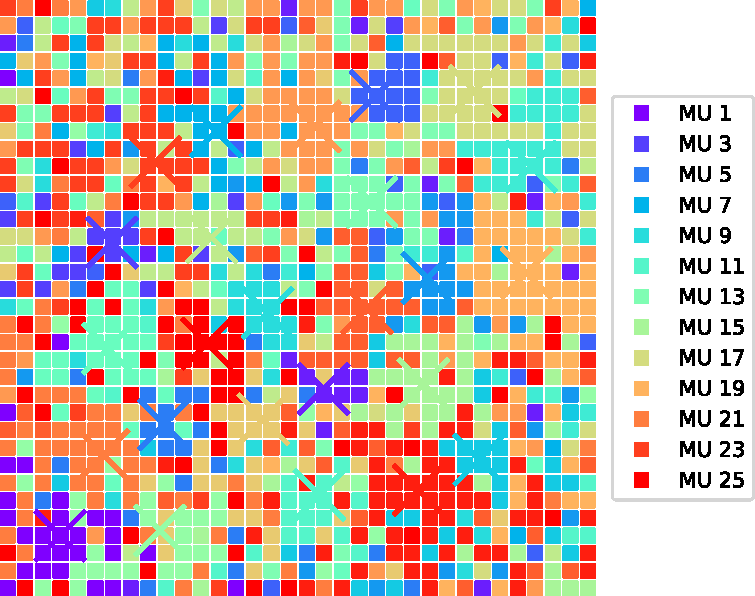
\includegraphics[width=\textwidth]{images/motor_unit_assignment/MU_fibre_distribution_combined_67x67_100_0_2d_fiber_distribution_.pdf}%
    \caption{First partial grid, $n=34$.}%
    \label{fig:mu_3partial_1}%
  \end{subfigure}
  \,
  \begin{subfigure}[t]{0.48\textwidth}%
    \centering%
    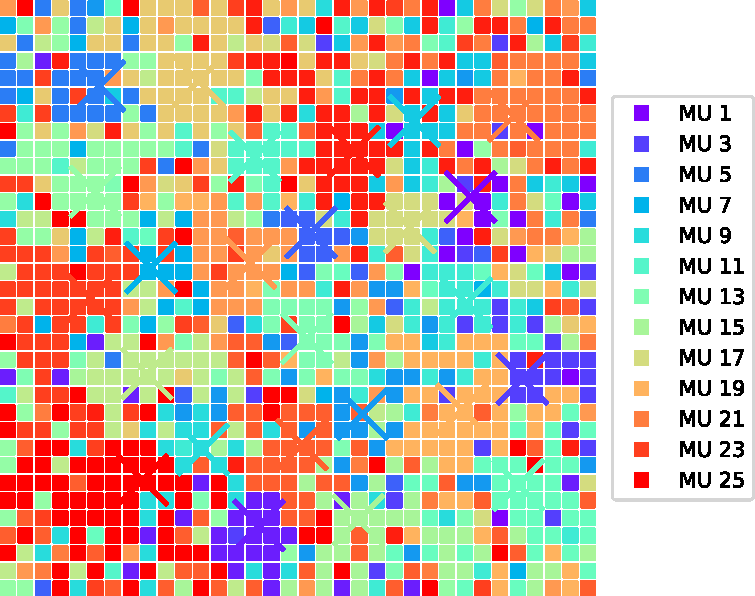
\includegraphics[width=\textwidth]{images/motor_unit_assignment/MU_fibre_distribution_combined_67x67_100_1_2d_fiber_distribution_.pdf}%
    \caption{Second partial grid, $n=34$.}%
    \label{fig:mu_3partial_2}%
  \end{subfigure}
  \,
  \begin{subfigure}[t]{0.48\textwidth}%
    \centering%
    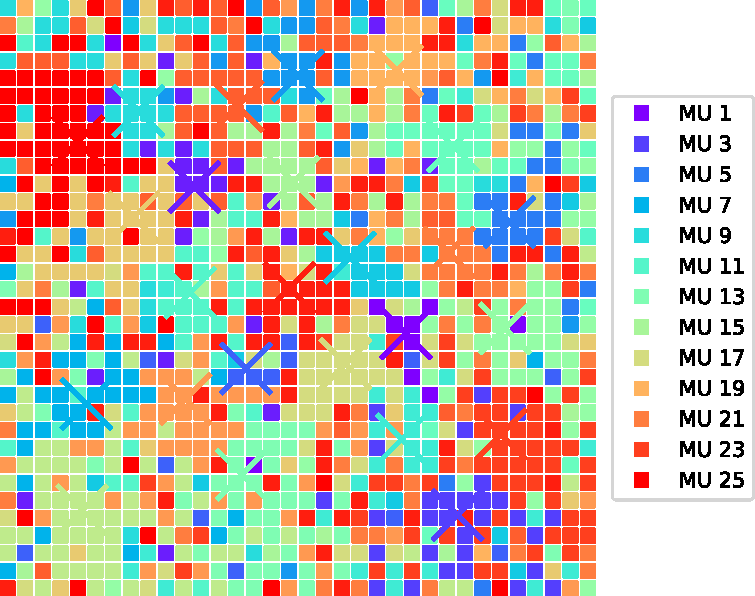
\includegraphics[width=\textwidth]{images/motor_unit_assignment/MU_fibre_distribution_combined_67x67_100_2_2d_fiber_distribution_.pdf}%
    \caption{Third partial grid, $n=34$.}%
    \label{fig:mu_3partial_3}%
  \end{subfigure}
  \,
%  \begin{subfigure}[t]{0.48\textwidth}%
%    \centering%
%    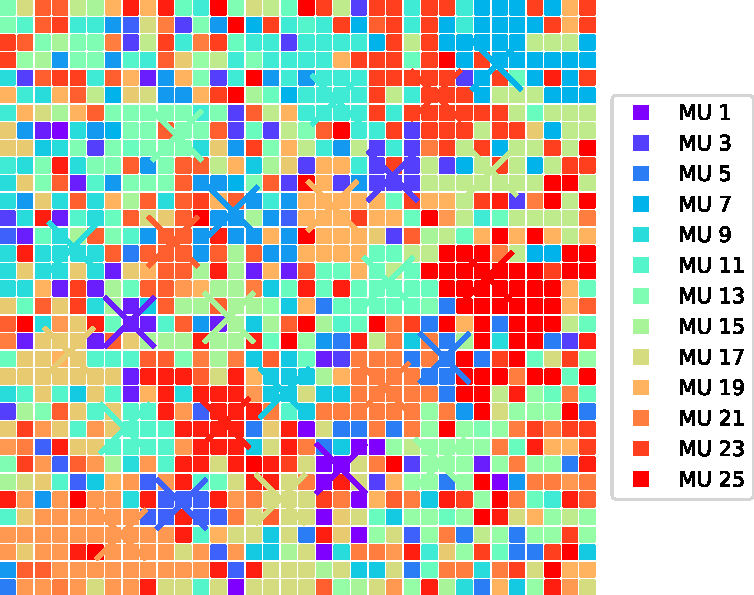
\includegraphics[width=\textwidth]{images/motor_unit_assignment/MU_fibre_distribution_combined_67x67_100_3_2d_fiber_distribution_.pdf}%
%    \caption{Forth partial grid.}%
%    \label{fig:mu_3partial_4}%
%  \end{subfigure}
  \begin{subfigure}[t]{0.48\textwidth}%
    \centering%
    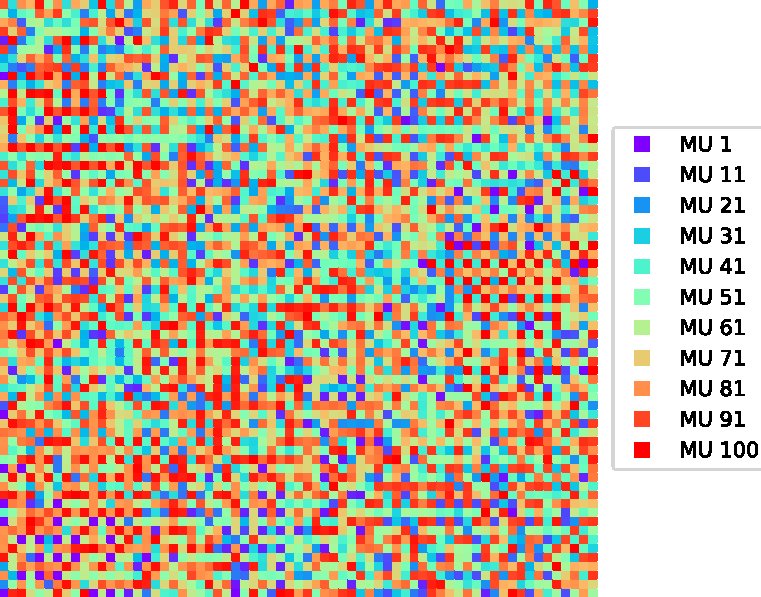
\includegraphics[width=\textwidth]{images/motor_unit_assignment/MU_fibre_distribution_combined_67x67_100_2d_fiber_distribution_.pdf}%
    \caption{Resulting interleaved grid, $n=67$.}%
    \label{fig:mu_3_1}%
  \end{subfigure}
  \caption{Assignment of motor units to fibers using method 1a. Shown are the first three partial grids (a)-(c) to be interleaved and the result (d), parameters $n=67, n_\text{MU}=100, \sigma = n/10 = 6.7, b=1.05$}%
  \label{fig:mu_method3_partial}%
\end{figure}%


\begin{figure}%
  \centering
  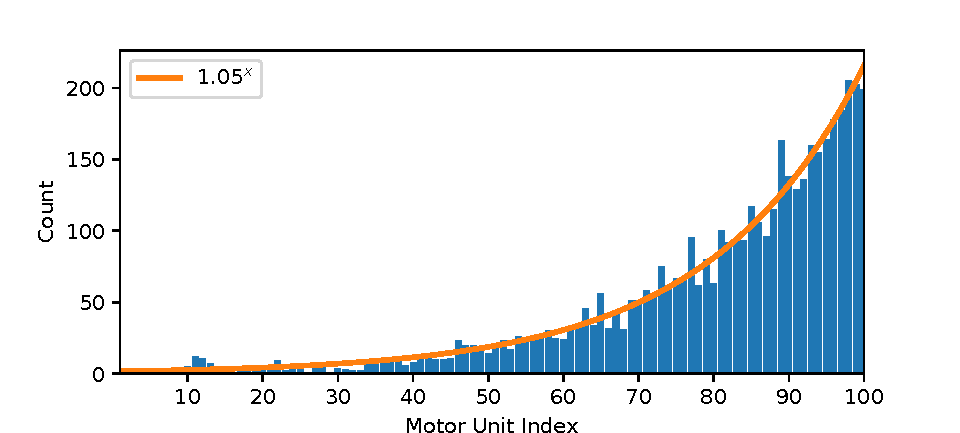
\includegraphics[width=0.9\textwidth]{images/motor_unit_assignment/MU_fibre_distribution_combined_67x67_100_fiber_distribution.pdf}%
  \caption{Histogram of number of fibers assigned to MUs for method 1a, for the scenario that is shown in \cref{fig:mu_method3_partial}.}%
  \label{fig:mu_method3_distribution}%
\end{figure}%

Method 2a cannot be reasonably used with the same parameters as method 1a. If it is used to generate fibers assigned to 100 MUs, a grid of $67 \times 67$ leads to the majority of MUs having only 1 fiber. Therefore, a larger grid is needed. \Cref{fig:mu_method3_2} shows the result for $n=251$. The result assigns \num{13618} of the $n^2 = \num{63001}$ initial fibers to MUs, i.e. \SI{22}{\percent}. The number of fibers per MU varies between \num{41} and \num{244}. As can be seen, fibers of the same MU are separated by either a fiber of a different MU or by a an unassigned fiber, i.e., a hole in the grid.

%It can be seen in \cref{fig:mu_method3_2} that the fibers are dispersed over the grid and holes are present throughout the domain. The resulting set of fibers can be viewed as being arbitrarily positioned in the domain instead of following the grid. When this viewpoint is adopted, the property that neighboring fibers are of different MUs no longer holds as the separation is often given by a hole, which does not prevent the fibers touching each other.

\begin{figure}%
  \centering
  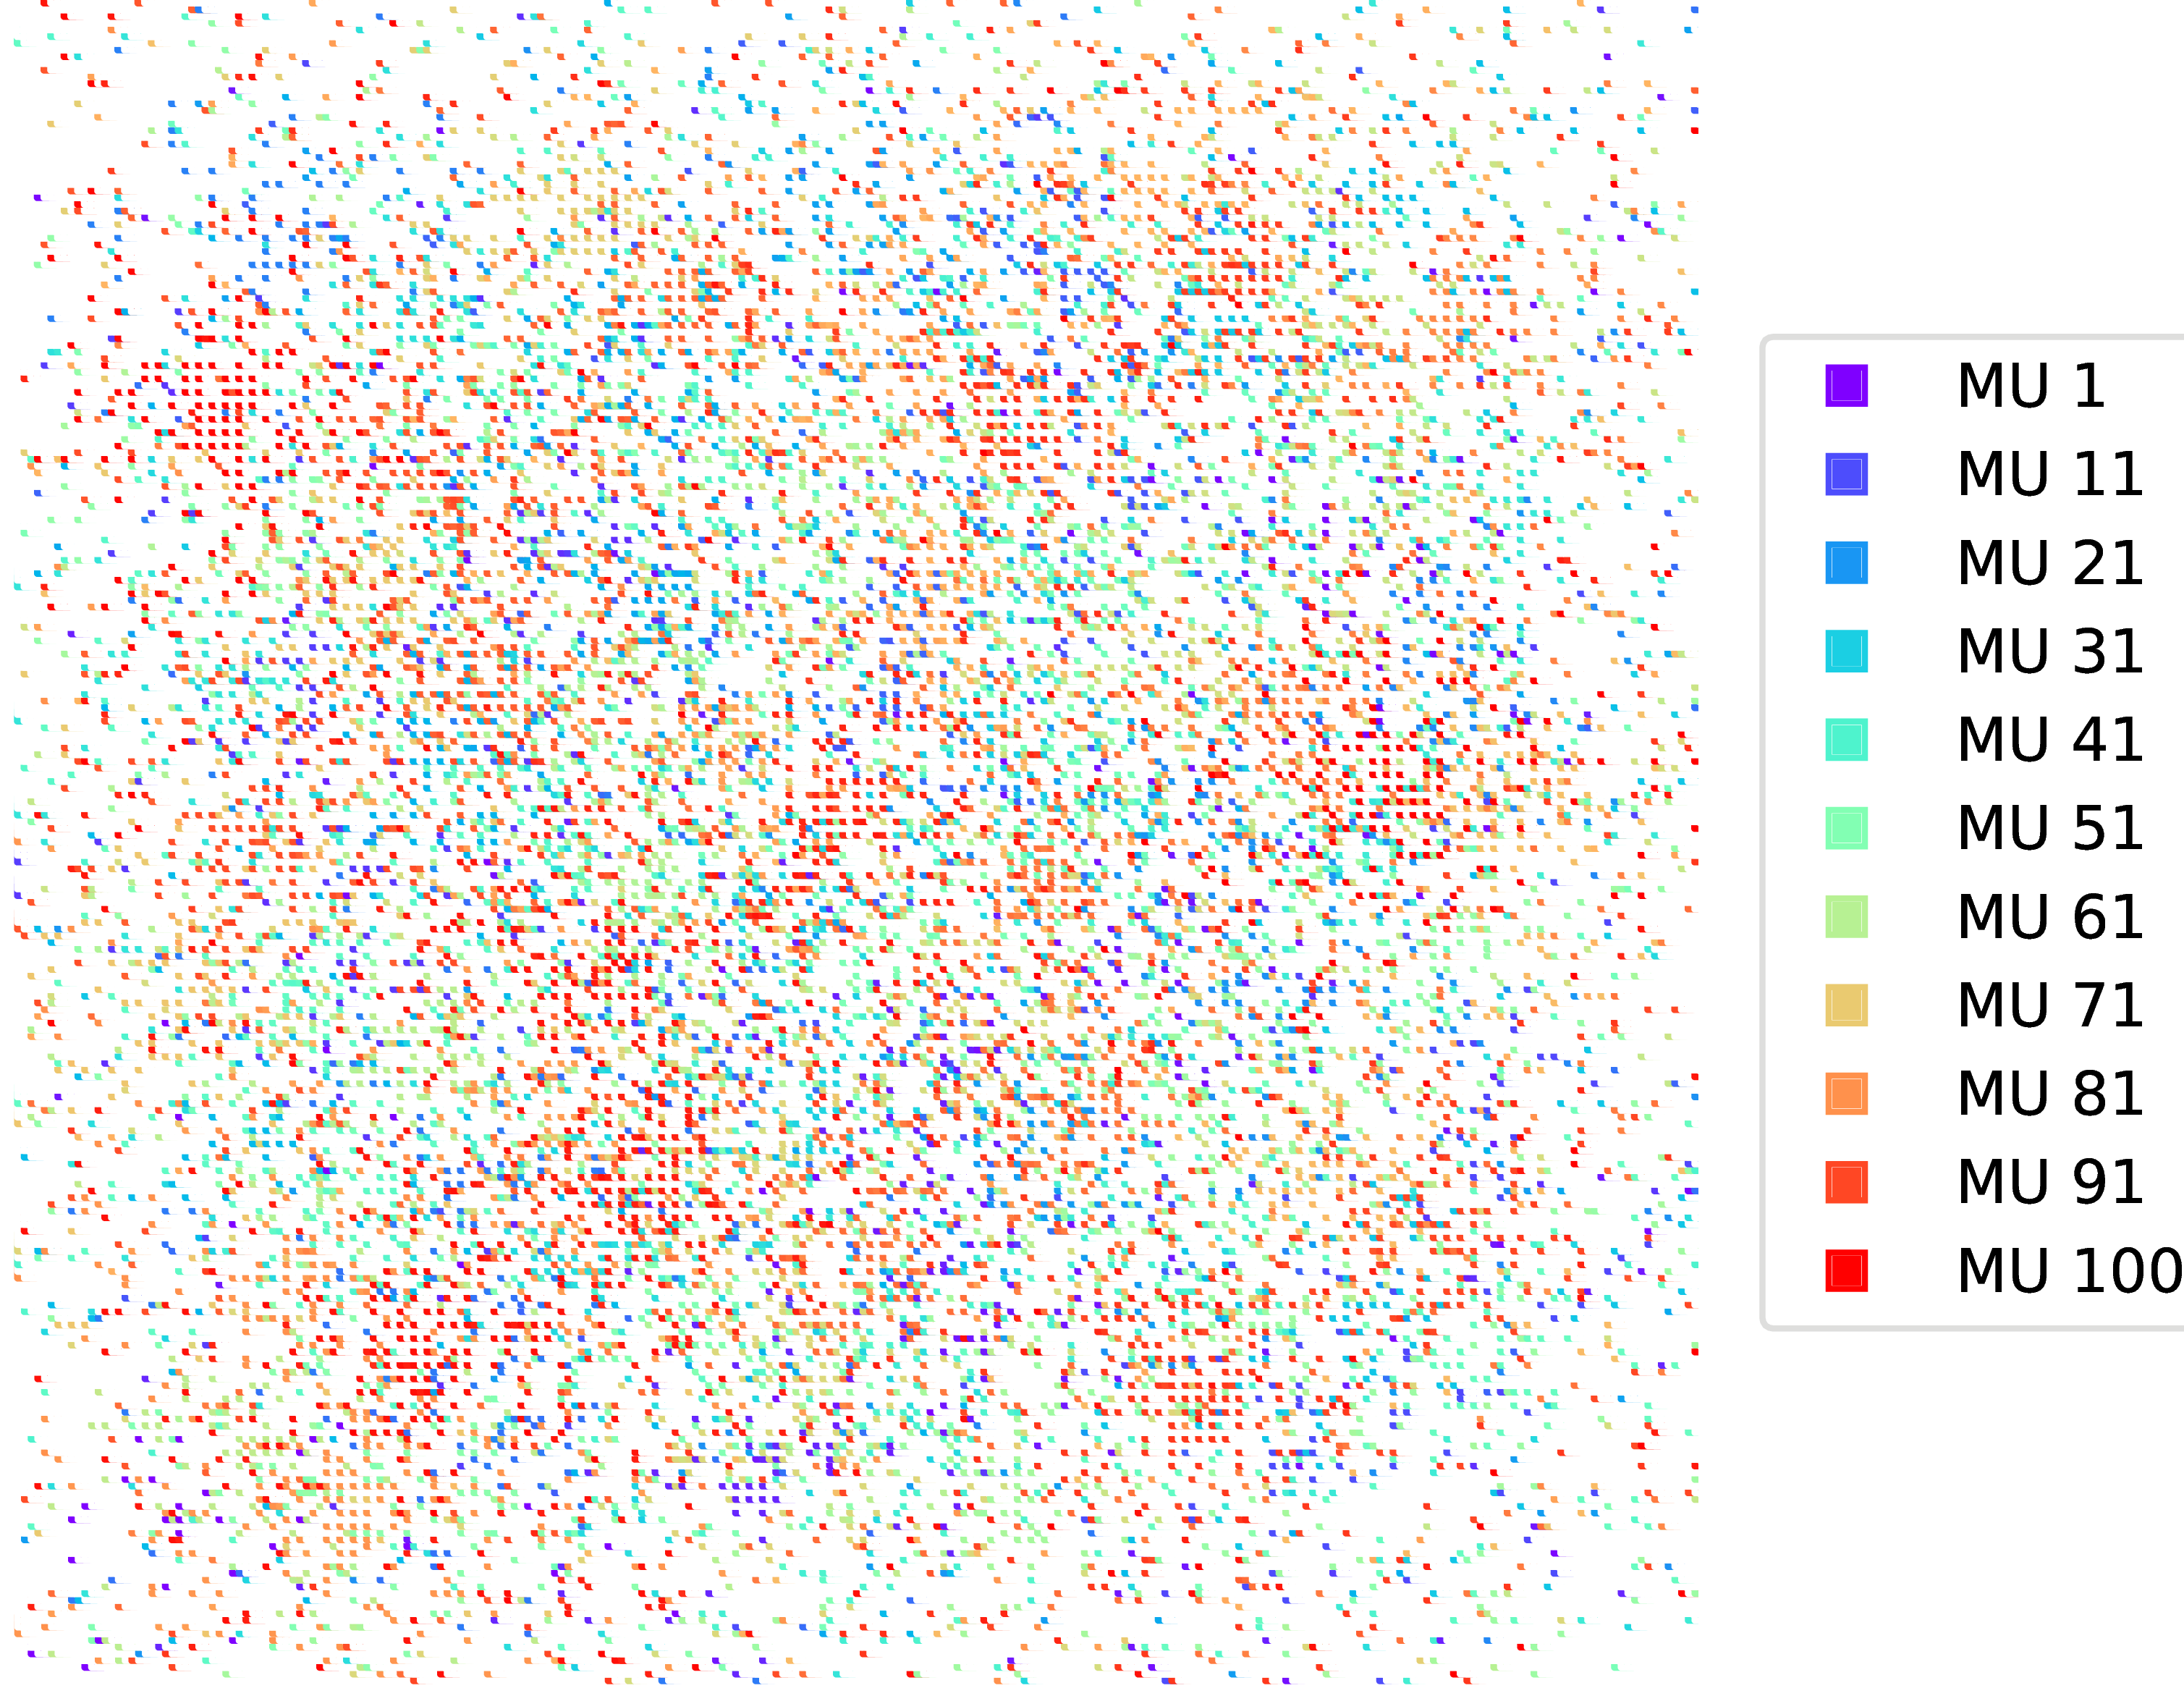
\includegraphics[width=0.9\textwidth]{images/motor_unit_assignment/MU_fibre_distribution_combined_sparse_251x251_100_2d_fiber_distribution_.png}%
  \caption{Assignment of motor units to fibers using method 2a and parameters $n=251, n_\text{MU}=100, \sigma = n/100 = 2.51, b=1.05$.}%
  \label{fig:mu_method3_2}%
\end{figure}%
% resulting fibers: 13618 / 63001 = 22\%

\begin{reproduce}
  Run the script \code{generate_fiber_distribution.py} without arguments to get usage information.
  The script contains the implementation for all three presented methods. For example, to run method 1a to get the result of \cref{fig:mu_method3_partial}, use:
  \begin{lstlisting}[columns=fullflexible,breaklines=true,postbreak=\mbox{\textcolor{gray}{$\hookrightarrow$}\space}]
    generate_fiber_distribution.py MU_fibre_distribution_combined_67x67_100 100 3 1 67 1.05 100 10
  \end{lstlisting}
  Then, existing fiber distribution files can be visualized by the following script:
  \begin{lstlisting}[columns=fullflexible,breaklines=true,postbreak=\mbox{\textcolor{gray}{$\hookrightarrow$}\space}]
    $\$$OPENDIHU_HOME/examples/electrophysiology/input/plot_fibre_distribution_2d.py MU_fibre_distribution_combined_67x67_100.txt 67
  \end{lstlisting}
\end{reproduce}

\section{Summary and Conclusion}\label{sec:mu_conclusion}
In the beginning of this chapter, two methods 1 and 2 for associating MUs with fibers in a given 2D grid were presented. The methods were constructed based on biophysical properties of MU distribution. The fibers were located in intermingling MU territories that were each centered at different MU center points.
The density of fibers belonging to an MU decreased with higher distance from the center and was described by a radial kernel function.
The number of fibers assigned to the motor units approximately followed an exponential progression where the first MU contained the lowest number of fibers and the last MU contained the largest amount. 
Whereas method 1 assigned MUs to all available fibers, method 2 only assigned MUs to some fibers yielding a lower number of fibers in the result.
Evaluation of the literature showed that no comparable method with these properties existed previously.

Next, the methods 1a and 2a were introduced that built upon methods 1 and 2. They ensured that neighboring fibers were assigned to different MUs, another behaviour that was known from anatomical studies.

Steps of the algorithms and their final satisfaction of the design critera were demonstrated with various visualizations. Results were shown for different parameter values. The influence of the kernel width on the \say{sharpness} or intermingledness of MU territories was pointed out. 

It was found that methods 2 and 2a typically produced results where only 20-50\% of the fibers get an MU assigned. This ratio highly depended on the problem size and the kernel function width and no direct predictions about the number of resulting fibers was possible. Since the kernel parameter at the same time also influenced the sharpness of the MU territories, adjusting parameters to the desired outcome was an issue for these methods. Reasonable results were only achieved for a higher number of initial fibers. In contrast, methods 1 and 1a robustly produced exponentially distributed MU assignments for all parameter values.

In method 2a for large grid sizes the fibers were dispersed over the grid and \say{holes}, i.e., unassigned fibers, were present throughout the domain. The fiber density decreased towards the boundaries of the domain. No experimental evidence exists that this behaviour occurs in reality. It might also be unfavorable when EMG simulations are performed where the boundary layers contribute most to the measured EMG signal on the muscle surface. In contrary, method 1a did not show this behaviour.

The runtime for \num{4489} fibers and 100 MUs was over \SI{45}{\min} for method 1 and below \SI{10}{\sec} for method 2. The large difference could be explained with the optimization problem that needed to be solved for method 1. To handle large runtimes for a high number of MUs, an algorithm was presented that splits the optimization problem in smaller chunks that could be solved faster.

With the use of the extended methods 1a and 1b, runtime decreased. For method 1a the runtime was under \SI{6}{\min}. These runtimes are all considered acceptable since the task occurs only once during preprocessing. 

In conclusion, the developed method 1a proved to be robust for all tested parameter combinations and fulfilled all considered biophysical properties of MU distributions. The exponential distribution of MU sizes and the sharpness of MU territories are adjustable through parameters. If the condition that neighbouring fibers belong to different MUs is not desired, method 1 can be used instead.

The presented methods are implemented and made available as Open Source software within \opendihu{}.
The program stores the resulting MU assignments in a plain text file format that is compatible with both OpenCMISS Iron and \opendihu{}. Thus, it can and will be used in simulations of the multiscale chemo-electromechanical model.


% \chapter{Formulation of electrophysiology and muscle contraction}
%    - electrophysiology introduction
%    \section{State of the art}
%    - Hodgkin-Huxley, shorten, advanced models, how it gets solved
%    \section{discretization}
%    - discretization of electrophysiology, operator splitting
%    \section{Standard for formulation of models}
%    - cellml introduction
%    \section{Bidomain}
%    - EMG
%    \section{Multidomain}
%    - multidomain formulation
%    \section{Formulation of solid mechanics}
%    - basics solid mechanics framework, material modeling, 
%    
%    \section{Simulation workflow}
%    - simulation workflow of skeletal muscle
%  
% \chapter{Numerics}
%   \section{Fundamentals of the discretization}
%    \section{Finite element method}
%    - basics FEM formulation of Laplace operator and diffusion equation, boundary conditions
%    \section{Incompressible nonlinear solid mechanics}
%    - incompressibility, penalty formulation vs. mixed formulation\\
%    - governing nonlinear eq.\\
%    - jacobian
%   \section{Numerical schemes}
%    \section{time stepping schemes}
%    \section{linear system solvers}
%    \section{newton algorithm}
%  % 
% \chapter{Simulation software}
%    \section{State of the art}
%    - review on bioengineering simulation frameworks 
%    
%    \section{OpenCMISS}
%  - OpenCMISS introduction, iron zinc cmgui, unstructured\\
%  
%  - Strang splitting, solvers 1D\\
%  - improved interpolation\\
%  - parallelization, issue with 1D \\
%  - 3D parallelization strategies\\
%  - design flaws, memory\\
%    % untergliedern, z.B. schnittstellen parall etc.
%    \section{The simulation framework \emph{opendihu}}
%    - modularity of opendihu, concepts (python c++ build system)
%    \section{Overview of discretization features}
%    - feature overview, implemented equations, ansatz functions, meshes
%    \section{Input and output}
%    - file i/o parallel, i: only local data important for high parallelism, o: paraview
%    \section{In-situ visualization}
%    - in-situ
%    \section{Details on the implementation}
%    \section{Representation of structured meshes}
%    \section{Parallel data handling}
%    - data structures, petsc variables, partitioning, ghost communication
%    \section{Implementation of boundary conditions}
%    - Neumann, Dirichlet boundary conditions
%    \section{Implementation of material formulation and automatic derivation of derivatives}
%    - implementation of solid mechanics with analytic differentiation
%    
%    \section{efficient and configurable data transfer}
%    - data layout details, efficient transfer of variables between solvers
%    \section{Mapping between meshes}
%    - parallel mapping between meshes, invertability of index space represesantion
%    \section{An efficient solver to the Monodomain equation}    
%    - cellml code generator and its optimizations - openmp, simd, vc
%    \section{Details on the partitioning}
%    - fibers emg structure and partitioning
%    \section{Parallelization of the multidomain system}
%    - multidomain parallelization, reordering of matrix
%    \section{load balancing}
%    - load balancing on fiber level
% \chapter{External coupling}
%    - introduction to external coupling, precice
%    \section{coupling with FEBio}
%    \section{coupling with AceFEM}
%  

%  \chapter{An algorithm for mesh generation}
%    - introduction, need for fiber and 3d mesh
%    \section{State of the art}
%    - literature, laplace potential flow idea
%    \section{Data preprocessing}
%    - visual human dataset, methods to extract surface, approximation by spline surfaces
%    \section{Outline of the algorithm}
%    - pseudo code
%    \section{Plane mesh smoothing}
%    \section{Parallelization}
%    \section{Generation of fiber meshes}
%    - generation of muscle mesh, 3D and fibers, also in parallel
%  
% \chapter{Simulation scenarios}
%    \section{Simulation of electromyography with fiber-based formulation}
%      - scenario static-biceps-emg, composite meshes
%    \section{Simulation of electromyography with multidomain formulation}
%    \section{Muscle contraction with fiber-based formulation}
%      - fibers with contraction
%    \section{Muscle contraction with multidomain formulation}
% \chapter{Technical simulation results}
%    \section{Runtime evaluation}
%    - results and experiments, runtime, peak performance\\
%    - monodomain runtime comparison OpenCMISS opendihu
%    \section{parallel partitioning}
%    - parallel partitioning and weak scaling, opencmiss and opendihu 
%    \section{memory consumption}
%    - memory scaling OpenCMISS
% \chapter{biomechanical simulation results}
%    \section{Simulation of fatigue}
%    - monodomain, hh  shorten, fatigue effects
%    \section{Simulation of EMG}
%    - static biceps emg\\
%    - fibers with contraction\\
%    - multidomain with fat layer\\
%    - multidomain with contraction\\
%
%\part{Soft tissue robotics}
%\chapter{...}
%  - introduction, handling flexible objects, overview of different object types\\
%  - basics Lagrange formulation of cable\\
%  - cable with friction on surface\\
%  - placing cable\\
%  - peg-in-hole, with sparse grids\\
%  - simulation of 2d tissue\\
%  - gripping point estimation\\
%  
%  \cite{Maier2021}
%  
%\part{Conclusion}

% -------------- Literaturseite --------------------
\newpage

%\acsetup{pages/display=first,pages/name=true}

% Abbreviations
%\printacronyms[include-classes=abbrev,name=Abbreviations]

% Nomenclature
%\printacronyms[include-classes=nomencl,name=Nomenclature]


%\bibliography{references}{}
%\bibliographystyle{abbrv}
\printbibliography[%
  % change title
  title=Bibliography
]


% -------------- Anhang ------------
%\appendix
%\input{8_anhang.tex}

\end{document}

%\input{preambule/footer}
